\batchmode
\documentclass[twoside]{book}

% Packages required by doxygen
\usepackage{fixltx2e}
\usepackage{calc}
\usepackage{doxygen}
\usepackage[export]{adjustbox} % also loads graphicx
\usepackage{graphicx}
\usepackage[utf8]{inputenc}
\usepackage{makeidx}
\usepackage{multicol}
\usepackage{multirow}
\PassOptionsToPackage{warn}{textcomp}
\usepackage{textcomp}
\usepackage[nointegrals]{wasysym}
\usepackage[table]{xcolor}

% Font selection
\usepackage[T1]{fontenc}
\usepackage[scaled=.90]{helvet}
\usepackage{courier}
\usepackage{amssymb}
\usepackage{sectsty}
\renewcommand{\familydefault}{\sfdefault}
\allsectionsfont{%
  \fontseries{bc}\selectfont%
  \color{darkgray}%
}
\renewcommand{\DoxyLabelFont}{%
  \fontseries{bc}\selectfont%
  \color{darkgray}%
}
\newcommand{\+}{\discretionary{\mbox{\scriptsize$\hookleftarrow$}}{}{}}

% Page & text layout
\usepackage{geometry}
\geometry{%
  a4paper,%
  top=2.5cm,%
  bottom=2.5cm,%
  left=2.5cm,%
  right=2.5cm%
}
\tolerance=750
\hfuzz=15pt
\hbadness=750
\setlength{\emergencystretch}{15pt}
\setlength{\parindent}{0cm}
\setlength{\parskip}{3ex plus 2ex minus 2ex}
\makeatletter
\renewcommand{\paragraph}{%
  \@startsection{paragraph}{4}{0ex}{-1.0ex}{1.0ex}{%
    \normalfont\normalsize\bfseries\SS@parafont%
  }%
}
\renewcommand{\subparagraph}{%
  \@startsection{subparagraph}{5}{0ex}{-1.0ex}{1.0ex}{%
    \normalfont\normalsize\bfseries\SS@subparafont%
  }%
}
\makeatother

% Headers & footers
\usepackage{fancyhdr}
\pagestyle{fancyplain}
\fancyhead[LE]{\fancyplain{}{\bfseries\thepage}}
\fancyhead[CE]{\fancyplain{}{}}
\fancyhead[RE]{\fancyplain{}{\bfseries\leftmark}}
\fancyhead[LO]{\fancyplain{}{\bfseries\rightmark}}
\fancyhead[CO]{\fancyplain{}{}}
\fancyhead[RO]{\fancyplain{}{\bfseries\thepage}}
\fancyfoot[LE]{\fancyplain{}{}}
\fancyfoot[CE]{\fancyplain{}{}}
\fancyfoot[RE]{\fancyplain{}{\bfseries\scriptsize Generated by Doxygen }}
\fancyfoot[LO]{\fancyplain{}{\bfseries\scriptsize Generated by Doxygen }}
\fancyfoot[CO]{\fancyplain{}{}}
\fancyfoot[RO]{\fancyplain{}{}}
\renewcommand{\footrulewidth}{0.4pt}
\renewcommand{\chaptermark}[1]{%
  \markboth{#1}{}%
}
\renewcommand{\sectionmark}[1]{%
  \markright{\thesection\ #1}%
}

% Indices & bibliography
\usepackage{natbib}
\usepackage[titles]{tocloft}
\setcounter{tocdepth}{3}
\setcounter{secnumdepth}{5}
\makeindex

% Hyperlinks (required, but should be loaded last)
\usepackage{ifpdf}
\ifpdf
  \usepackage[pdftex,pagebackref=true]{hyperref}
\else
  \usepackage[ps2pdf,pagebackref=true]{hyperref}
\fi
\hypersetup{%
  colorlinks=true,%
  linkcolor=blue,%
  citecolor=blue,%
  unicode%
}

% Custom commands
\newcommand{\clearemptydoublepage}{%
  \newpage{\pagestyle{empty}\cleardoublepage}%
}

\usepackage{caption}
\captionsetup{labelsep=space,justification=centering,font={bf},singlelinecheck=off,skip=4pt,position=top}

%===== C O N T E N T S =====

\begin{document}

% Titlepage & ToC
\hypersetup{pageanchor=false,
             bookmarksnumbered=true,
             pdfencoding=unicode
            }
\pagenumbering{alph}
\pagenumbering{arabic}
\hypersetup{pageanchor=true}

%--- Begin generated contents ---
\chapter{Segregated solvers for fluid-\/structure-\/interaction problems\+: Revisiting the flow in a 2D collapsible channel}
\label{index}\hypertarget{index}{}\hypertarget{index_q}{}\section{A few quick questions...}\label{index_q}
Since {\ttfamily oomph-\/lib} is developed as open-\/source software, any evidence that the code is being downloaded and used is very helpful for us as it helps to justify our continued work on this project.

We would therefore be extremely grateful if you could provide the information requested in the form below. Pressing the \char`\"{}submit\char`\"{} button will get you to the actual download page.

{\bfseries Note\+:} 
\begin{DoxyItemize}
\item All information will be treated as confidential. 
\item If you provide your email address and check the appropriate box we will add you to our mailing list to inform you of upgrades and bug fixes to the code. Rest assured that the mailing list is {\bfseries very low volume} -- we have better things to do than to bombard you with email. 
\item If you still feel reluctant to provide any of the information requested, feel free to enter some dummy input. The form will check that {\bfseries some} information has been entered but entering your name as \char`\"{}\+Joe Cool\char`\"{} is perfectly acceptable -- this is to discourage people from not providing the information simply because they are too lazy to type... 
\end{DoxyItemize}



 







 

 \hypertarget{index_pdf}{}\section{P\+D\+F file}\label{index_pdf}
A \href{../latex/refman.pdf}{\tt pdf version} of this document is available. \end{document}

\chapter{Namespace Index}
\section{Namespace List}
Here is a list of all namespaces with brief descriptions\+:\begin{DoxyCompactList}
\item\contentsline{section}{\hyperlink{namespaceGlobal__Physical__Variables}{Global\+\_\+\+Physical\+\_\+\+Variables} \\*Global variables that represent physical properties }{\pageref{namespaceGlobal__Physical__Variables}}{}
\item\contentsline{section}{\hyperlink{namespaceoomph}{oomph} }{\pageref{namespaceoomph}}{}
\item\contentsline{section}{\hyperlink{namespacePhysical__Variables}{Physical\+\_\+\+Variables} \\*Namespace for the solution of 2D linear shell equation }{\pageref{namespacePhysical__Variables}}{}
\end{DoxyCompactList}

\chapter{Hierarchical Index}
\section{Class Hierarchy}
This inheritance list is sorted roughly, but not completely, alphabetically\+:\begin{DoxyCompactList}
\item Problem\begin{DoxyCompactList}
\item \contentsline{section}{Unstructured\+Solid\+Problem$<$ E\+L\+E\+M\+E\+NT $>$}{\pageref{classUnstructuredSolidProblem}}{}
\end{DoxyCompactList}
\end{DoxyCompactList}

\chapter{Class Index}
\section{Class List}
Here are the classes, structs, unions and interfaces with brief descriptions\+:\begin{DoxyCompactList}
\item\contentsline{section}{\hyperlink{classPMLProblem}{P\+M\+L\+Problem$<$ E\+L\+E\+M\+E\+N\+T $>$} }{\pageref{classPMLProblem}}{}
\item\contentsline{section}{\hyperlink{classGlobalParameters_1_1TestPMLMapping}{Global\+Parameters\+::\+Test\+P\+M\+L\+Mapping} }{\pageref{classGlobalParameters_1_1TestPMLMapping}}{}
\end{DoxyCompactList}

\chapter{File Index}
\section{File List}
Here is a list of all files with brief descriptions\+:\begin{DoxyCompactList}
\item\contentsline{section}{\hyperlink{jeffery__orbit_8cc}{jeffery\+\_\+orbit.\+cc} }{\pageref{jeffery__orbit_8cc}}{}
\item\contentsline{section}{\hyperlink{jeffery__orbit_8txt__doxygenified_8h}{jeffery\+\_\+orbit.\+txt\+\_\+doxygenified.\+h} }{\pageref{jeffery__orbit_8txt__doxygenified_8h}}{}
\item\contentsline{section}{\hyperlink{my__taylor__hood__elements_8h}{my\+\_\+taylor\+\_\+hood\+\_\+elements.\+h} }{\pageref{my__taylor__hood__elements_8h}}{}
\end{DoxyCompactList}

\chapter{Namespace Documentation}
\hypertarget{namespaceBL__Squash}{}\section{B\+L\+\_\+\+Squash Namespace Reference}
\label{namespaceBL__Squash}\index{B\+L\+\_\+\+Squash@{B\+L\+\_\+\+Squash}}
\subsection*{Functions}
\begin{DoxyCompactItemize}
\item 
double \hyperlink{namespaceBL__Squash_a0fdaf7661591150041b7102dbe578cdc}{squash\+\_\+fct} (const double \&s)
\begin{DoxyCompactList}\small\item\em Mapping \mbox{[}0,1\mbox{]} -\/$>$ \mbox{[}0,1\mbox{]} that re-\/distributes nodal points across the channel width. \end{DoxyCompactList}\end{DoxyCompactItemize}
\subsection*{Variables}
\begin{DoxyCompactItemize}
\item 
double \hyperlink{namespaceBL__Squash_a3c4183891049bca81f3a011db24fc579}{Delta} =0.\+1
\begin{DoxyCompactList}\small\item\em Boundary layer width. \end{DoxyCompactList}\item 
double \hyperlink{namespaceBL__Squash_af84bda39008884cd2b01e630957573df}{Fract\+\_\+in\+\_\+\+BL} =0.\+5
\begin{DoxyCompactList}\small\item\em Fraction of points in boundary layer. \end{DoxyCompactList}\end{DoxyCompactItemize}


\subsection{Detailed Description}
Namespace to define the mapping \mbox{[}0,1\mbox{]} -\/$>$ \mbox{[}0,1\mbox{]} that re-\/distributes nodal points across the channel width. 

\subsection{Function Documentation}
\mbox{\Hypertarget{namespaceBL__Squash_a0fdaf7661591150041b7102dbe578cdc}\label{namespaceBL__Squash_a0fdaf7661591150041b7102dbe578cdc}} 
\index{B\+L\+\_\+\+Squash@{B\+L\+\_\+\+Squash}!squash\+\_\+fct@{squash\+\_\+fct}}
\index{squash\+\_\+fct@{squash\+\_\+fct}!B\+L\+\_\+\+Squash@{B\+L\+\_\+\+Squash}}
\subsubsection{\texorpdfstring{squash\+\_\+fct()}{squash\_fct()}}
{\footnotesize\ttfamily double B\+L\+\_\+\+Squash\+::squash\+\_\+fct (\begin{DoxyParamCaption}\item[{const double \&}]{s }\end{DoxyParamCaption})}



Mapping \mbox{[}0,1\mbox{]} -\/$>$ \mbox{[}0,1\mbox{]} that re-\/distributes nodal points across the channel width. 



Definition at line 63 of file fsi\+\_\+collapsible\+\_\+channel.\+cc.



References Delta, and Fract\+\_\+in\+\_\+\+BL.



Referenced by Elastic\+Collapsible\+Channel\+Mesh$<$ E\+L\+E\+M\+E\+N\+T $>$\+::\+Elastic\+Collapsible\+Channel\+Mesh(), Elastic\+Refineable\+Collapsible\+Channel\+Mesh$<$ E\+L\+E\+M\+E\+N\+T $>$\+::\+Elastic\+Refineable\+Collapsible\+Channel\+Mesh(), and F\+S\+I\+Collapsible\+Channel\+Problem$<$ E\+L\+E\+M\+E\+N\+T $>$\+::\+F\+S\+I\+Collapsible\+Channel\+Problem().



\subsection{Variable Documentation}
\mbox{\Hypertarget{namespaceBL__Squash_a3c4183891049bca81f3a011db24fc579}\label{namespaceBL__Squash_a3c4183891049bca81f3a011db24fc579}} 
\index{B\+L\+\_\+\+Squash@{B\+L\+\_\+\+Squash}!Delta@{Delta}}
\index{Delta@{Delta}!B\+L\+\_\+\+Squash@{B\+L\+\_\+\+Squash}}
\subsubsection{\texorpdfstring{Delta}{Delta}}
{\footnotesize\ttfamily double B\+L\+\_\+\+Squash\+::\+Delta =0.\+1}



Boundary layer width. 



Definition at line 56 of file fsi\+\_\+collapsible\+\_\+channel.\+cc.



Referenced by Elastic\+Collapsible\+Channel\+Mesh$<$ E\+L\+E\+M\+E\+N\+T $>$\+::\+Elastic\+Collapsible\+Channel\+Mesh(), Elastic\+Refineable\+Collapsible\+Channel\+Mesh$<$ E\+L\+E\+M\+E\+N\+T $>$\+::\+Elastic\+Refineable\+Collapsible\+Channel\+Mesh(), and squash\+\_\+fct().

\mbox{\Hypertarget{namespaceBL__Squash_af84bda39008884cd2b01e630957573df}\label{namespaceBL__Squash_af84bda39008884cd2b01e630957573df}} 
\index{B\+L\+\_\+\+Squash@{B\+L\+\_\+\+Squash}!Fract\+\_\+in\+\_\+\+BL@{Fract\+\_\+in\+\_\+\+BL}}
\index{Fract\+\_\+in\+\_\+\+BL@{Fract\+\_\+in\+\_\+\+BL}!B\+L\+\_\+\+Squash@{B\+L\+\_\+\+Squash}}
\subsubsection{\texorpdfstring{Fract\+\_\+in\+\_\+\+BL}{Fract\_in\_BL}}
{\footnotesize\ttfamily double B\+L\+\_\+\+Squash\+::\+Fract\+\_\+in\+\_\+\+BL =0.\+5}



Fraction of points in boundary layer. 



Definition at line 59 of file fsi\+\_\+collapsible\+\_\+channel.\+cc.



Referenced by Elastic\+Collapsible\+Channel\+Mesh$<$ E\+L\+E\+M\+E\+N\+T $>$\+::\+Elastic\+Collapsible\+Channel\+Mesh(), Elastic\+Refineable\+Collapsible\+Channel\+Mesh$<$ E\+L\+E\+M\+E\+N\+T $>$\+::\+Elastic\+Refineable\+Collapsible\+Channel\+Mesh(), and squash\+\_\+fct().


\hypertarget{namespaceFlags}{}\section{Flags Namespace Reference}
\label{namespaceFlags}\index{Flags@{Flags}}


Extend namespace for control flags.  


\subsection*{Functions}
\begin{DoxyCompactItemize}
\item 
void \hyperlink{namespaceFlags_aa7e90522c3f7fbac06fa93f61d88bbd8}{doc\+\_\+flags} ()
\begin{DoxyCompactList}\small\item\em Doc flags. \end{DoxyCompactList}\end{DoxyCompactItemize}
\subsection*{Variables}
\begin{DoxyCompactItemize}
\item 
unsigned \hyperlink{namespaceFlags_a2cdfa6b776b959a060a1f2e8d4918789}{Use\+\_\+segregated\+\_\+solver} =1
\begin{DoxyCompactList}\small\item\em Use Newton solver (0) or segregated solver (1)? \end{DoxyCompactList}\item 
unsigned \hyperlink{namespaceFlags_aabfbfdb3e91e4df3fc2ec6e2a2e3567d}{Use\+\_\+pointwise\+\_\+aitken} =0
\begin{DoxyCompactList}\small\item\em Use pointwise Aitken extrapolation (1) or not (0) \end{DoxyCompactList}\item 
double \hyperlink{namespaceFlags_a6c3895aecba834ceda5fe1c3ecb13bba}{Omega\+\_\+under\+\_\+relax} =1.\+0
\begin{DoxyCompactList}\small\item\em Under-\/relaxation parameter (1.\+0\+: no under-\/relaxation; 0.\+0\+: freeze) \end{DoxyCompactList}\item 
unsigned \hyperlink{namespaceFlags_a9d92a2ec6ebd4e2ea66605c063e53915}{Use\+\_\+irons\+\_\+and\+\_\+tuck\+\_\+extrapolation} =0
\begin{DoxyCompactList}\small\item\em Use Irons and Tuck extrapolation (1) or not (0) \end{DoxyCompactList}\item 
unsigned \hyperlink{namespaceFlags_aba930ff1e462e642a27904df95baab7c}{Convergence\+\_\+criterion} =0
\begin{DoxyCompactList}\small\item\em Convergence criterion\+: 0\+: global resmax; 1\+: abs. change; 2\+: rel. change. \end{DoxyCompactList}\item 
double \hyperlink{namespaceFlags_a5550ee43b27fd03898a6718246b44e4a}{Convergence\+\_\+tolerance} =1.\+0e-\/8
\begin{DoxyCompactList}\small\item\em Convergence tolerance. \end{DoxyCompactList}\item 
unsigned \hyperlink{namespaceFlags_a7c2437aa0b6a4f27df951f1cbcef7337}{Resolution\+\_\+factor} =1
\begin{DoxyCompactList}\small\item\em Resolution factor (multiplier for number of elements across channel) \end{DoxyCompactList}\item 
unsigned \hyperlink{namespaceFlags_adf4a2f4076156f633f45155a2d9f67a0}{Use\+\_\+displ\+\_\+control} =1
\begin{DoxyCompactList}\small\item\em Use displacement control (1) or not (0) \end{DoxyCompactList}\item 
unsigned \hyperlink{namespaceFlags_a94cadbe3202fa6f29b6aa5e7b491a9ae}{Steady\+\_\+flag} =1
\begin{DoxyCompactList}\small\item\em Steady run (1) or unsteady run (0) \end{DoxyCompactList}\item 
unsigned \hyperlink{namespaceFlags_a8a6ffdb261330ef89965624209ab7b00}{Nsteps} =5
\begin{DoxyCompactList}\small\item\em Number of steps in parameter study. \end{DoxyCompactList}\item 
string \hyperlink{namespaceFlags_a4401f7e5174d2dc44ec0e7a0d94869af}{Run\+\_\+identifier\+\_\+string} =\char`\"{}\char`\"{}
\begin{DoxyCompactList}\small\item\em String to identify the run type in trace file. \end{DoxyCompactList}\item 
string \hyperlink{namespaceFlags_a3657ad4e287c8756f096b2abe1277cf3}{Restart\+\_\+file\+\_\+name} =\char`\"{}\char`\"{}
\begin{DoxyCompactList}\small\item\em Name of restart file. \end{DoxyCompactList}\end{DoxyCompactItemize}


\subsection{Detailed Description}
Extend namespace for control flags. 

Namespace for flags. 

\subsection{Function Documentation}
\mbox{\Hypertarget{namespaceFlags_aa7e90522c3f7fbac06fa93f61d88bbd8}\label{namespaceFlags_aa7e90522c3f7fbac06fa93f61d88bbd8}} 
\index{Flags@{Flags}!doc\+\_\+flags@{doc\+\_\+flags}}
\index{doc\+\_\+flags@{doc\+\_\+flags}!Flags@{Flags}}
\subsubsection{\texorpdfstring{doc\+\_\+flags()}{doc\_flags()}}
{\footnotesize\ttfamily void Flags\+::doc\+\_\+flags (\begin{DoxyParamCaption}{ }\end{DoxyParamCaption})}



Doc flags. 



Definition at line 258 of file fsi\+\_\+chan\+\_\+problem.\+h.



References Global\+\_\+\+Physical\+\_\+\+Variables\+::\+P\+\_\+step, Global\+\_\+\+Physical\+\_\+\+Variables\+::Q, and Global\+\_\+\+Physical\+\_\+\+Variables\+::\+Re.



\subsection{Variable Documentation}
\mbox{\Hypertarget{namespaceFlags_aba930ff1e462e642a27904df95baab7c}\label{namespaceFlags_aba930ff1e462e642a27904df95baab7c}} 
\index{Flags@{Flags}!Convergence\+\_\+criterion@{Convergence\+\_\+criterion}}
\index{Convergence\+\_\+criterion@{Convergence\+\_\+criterion}!Flags@{Flags}}
\subsubsection{\texorpdfstring{Convergence\+\_\+criterion}{Convergence\_criterion}}
{\footnotesize\ttfamily unsigned Flags\+::\+Convergence\+\_\+criterion =0}



Convergence criterion\+: 0\+: global resmax; 1\+: abs. change; 2\+: rel. change. 



Definition at line 70 of file simple\+\_\+segregated\+\_\+driver.\+cc.



Referenced by Segregated\+F\+S\+I\+Collapsible\+Channel\+Problem$<$ E\+L\+E\+M\+E\+N\+T $>$\+::\+Segregated\+F\+S\+I\+Collapsible\+Channel\+Problem().

\mbox{\Hypertarget{namespaceFlags_a5550ee43b27fd03898a6718246b44e4a}\label{namespaceFlags_a5550ee43b27fd03898a6718246b44e4a}} 
\index{Flags@{Flags}!Convergence\+\_\+tolerance@{Convergence\+\_\+tolerance}}
\index{Convergence\+\_\+tolerance@{Convergence\+\_\+tolerance}!Flags@{Flags}}
\subsubsection{\texorpdfstring{Convergence\+\_\+tolerance}{Convergence\_tolerance}}
{\footnotesize\ttfamily double Flags\+::\+Convergence\+\_\+tolerance =1.\+0e-\/8}



Convergence tolerance. 



Definition at line 73 of file simple\+\_\+segregated\+\_\+driver.\+cc.



Referenced by Segregated\+F\+S\+I\+Collapsible\+Channel\+Problem$<$ E\+L\+E\+M\+E\+N\+T $>$\+::\+Segregated\+F\+S\+I\+Collapsible\+Channel\+Problem().

\mbox{\Hypertarget{namespaceFlags_a8a6ffdb261330ef89965624209ab7b00}\label{namespaceFlags_a8a6ffdb261330ef89965624209ab7b00}} 
\index{Flags@{Flags}!Nsteps@{Nsteps}}
\index{Nsteps@{Nsteps}!Flags@{Flags}}
\subsubsection{\texorpdfstring{Nsteps}{Nsteps}}
{\footnotesize\ttfamily unsigned Flags\+::\+Nsteps =5}



Number of steps in parameter study. 



Definition at line 249 of file fsi\+\_\+chan\+\_\+problem.\+h.



Referenced by Segregated\+F\+S\+I\+Collapsible\+Channel\+Problem$<$ E\+L\+E\+M\+E\+N\+T $>$\+::steady\+\_\+run(), F\+S\+I\+Collapsible\+Channel\+Problem$<$ E\+L\+E\+M\+E\+N\+T $>$\+::steady\+\_\+run(), and F\+S\+I\+Collapsible\+Channel\+Problem$<$ E\+L\+E\+M\+E\+N\+T $>$\+::unsteady\+\_\+run().

\mbox{\Hypertarget{namespaceFlags_a6c3895aecba834ceda5fe1c3ecb13bba}\label{namespaceFlags_a6c3895aecba834ceda5fe1c3ecb13bba}} 
\index{Flags@{Flags}!Omega\+\_\+under\+\_\+relax@{Omega\+\_\+under\+\_\+relax}}
\index{Omega\+\_\+under\+\_\+relax@{Omega\+\_\+under\+\_\+relax}!Flags@{Flags}}
\subsubsection{\texorpdfstring{Omega\+\_\+under\+\_\+relax}{Omega\_under\_relax}}
{\footnotesize\ttfamily double Flags\+::\+Omega\+\_\+under\+\_\+relax =1.\+0}



Under-\/relaxation parameter (1.\+0\+: no under-\/relaxation; 0.\+0\+: freeze) 



Definition at line 64 of file simple\+\_\+segregated\+\_\+driver.\+cc.



Referenced by Segregated\+F\+S\+I\+Collapsible\+Channel\+Problem$<$ E\+L\+E\+M\+E\+N\+T $>$\+::\+Segregated\+F\+S\+I\+Collapsible\+Channel\+Problem().

\mbox{\Hypertarget{namespaceFlags_a7c2437aa0b6a4f27df951f1cbcef7337}\label{namespaceFlags_a7c2437aa0b6a4f27df951f1cbcef7337}} 
\index{Flags@{Flags}!Resolution\+\_\+factor@{Resolution\+\_\+factor}}
\index{Resolution\+\_\+factor@{Resolution\+\_\+factor}!Flags@{Flags}}
\subsubsection{\texorpdfstring{Resolution\+\_\+factor}{Resolution\_factor}}
{\footnotesize\ttfamily unsigned Flags\+::\+Resolution\+\_\+factor =1}



Resolution factor (multiplier for number of elements across channel) 



Definition at line 240 of file fsi\+\_\+chan\+\_\+problem.\+h.



Referenced by main(), F\+S\+I\+Collapsible\+Channel\+Problem$<$ E\+L\+E\+M\+E\+N\+T $>$\+::steady\+\_\+run(), and F\+S\+I\+Collapsible\+Channel\+Problem$<$ E\+L\+E\+M\+E\+N\+T $>$\+::unsteady\+\_\+run().

\mbox{\Hypertarget{namespaceFlags_a3657ad4e287c8756f096b2abe1277cf3}\label{namespaceFlags_a3657ad4e287c8756f096b2abe1277cf3}} 
\index{Flags@{Flags}!Restart\+\_\+file\+\_\+name@{Restart\+\_\+file\+\_\+name}}
\index{Restart\+\_\+file\+\_\+name@{Restart\+\_\+file\+\_\+name}!Flags@{Flags}}
\subsubsection{\texorpdfstring{Restart\+\_\+file\+\_\+name}{Restart\_file\_name}}
{\footnotesize\ttfamily string Flags\+::\+Restart\+\_\+file\+\_\+name =\char`\"{}\char`\"{}}



Name of restart file. 



Definition at line 255 of file fsi\+\_\+chan\+\_\+problem.\+h.



Referenced by F\+S\+I\+Collapsible\+Channel\+Problem$<$ E\+L\+E\+M\+E\+N\+T $>$\+::set\+\_\+initial\+\_\+condition().

\mbox{\Hypertarget{namespaceFlags_a4401f7e5174d2dc44ec0e7a0d94869af}\label{namespaceFlags_a4401f7e5174d2dc44ec0e7a0d94869af}} 
\index{Flags@{Flags}!Run\+\_\+identifier\+\_\+string@{Run\+\_\+identifier\+\_\+string}}
\index{Run\+\_\+identifier\+\_\+string@{Run\+\_\+identifier\+\_\+string}!Flags@{Flags}}
\subsubsection{\texorpdfstring{Run\+\_\+identifier\+\_\+string}{Run\_identifier\_string}}
{\footnotesize\ttfamily string Flags\+::\+Run\+\_\+identifier\+\_\+string =\char`\"{}\char`\"{}}



String to identify the run type in trace file. 



Definition at line 252 of file fsi\+\_\+chan\+\_\+problem.\+h.



Referenced by F\+S\+I\+Collapsible\+Channel\+Problem$<$ E\+L\+E\+M\+E\+N\+T $>$\+::steady\+\_\+run(), and F\+S\+I\+Collapsible\+Channel\+Problem$<$ E\+L\+E\+M\+E\+N\+T $>$\+::unsteady\+\_\+run().

\mbox{\Hypertarget{namespaceFlags_a94cadbe3202fa6f29b6aa5e7b491a9ae}\label{namespaceFlags_a94cadbe3202fa6f29b6aa5e7b491a9ae}} 
\index{Flags@{Flags}!Steady\+\_\+flag@{Steady\+\_\+flag}}
\index{Steady\+\_\+flag@{Steady\+\_\+flag}!Flags@{Flags}}
\subsubsection{\texorpdfstring{Steady\+\_\+flag}{Steady\_flag}}
{\footnotesize\ttfamily unsigned Flags\+::\+Steady\+\_\+flag =1}



Steady run (1) or unsteady run (0) 



Definition at line 246 of file fsi\+\_\+chan\+\_\+problem.\+h.



Referenced by F\+S\+I\+Collapsible\+Channel\+Problem$<$ E\+L\+E\+M\+E\+N\+T $>$\+::\+F\+S\+I\+Collapsible\+Channel\+Problem(), and F\+S\+I\+Collapsible\+Channel\+Problem$<$ E\+L\+E\+M\+E\+N\+T $>$\+::set\+\_\+initial\+\_\+condition().

\mbox{\Hypertarget{namespaceFlags_adf4a2f4076156f633f45155a2d9f67a0}\label{namespaceFlags_adf4a2f4076156f633f45155a2d9f67a0}} 
\index{Flags@{Flags}!Use\+\_\+displ\+\_\+control@{Use\+\_\+displ\+\_\+control}}
\index{Use\+\_\+displ\+\_\+control@{Use\+\_\+displ\+\_\+control}!Flags@{Flags}}
\subsubsection{\texorpdfstring{Use\+\_\+displ\+\_\+control}{Use\_displ\_control}}
{\footnotesize\ttfamily unsigned Flags\+::\+Use\+\_\+displ\+\_\+control =1}



Use displacement control (1) or not (0) 



Definition at line 243 of file fsi\+\_\+chan\+\_\+problem.\+h.

\mbox{\Hypertarget{namespaceFlags_a9d92a2ec6ebd4e2ea66605c063e53915}\label{namespaceFlags_a9d92a2ec6ebd4e2ea66605c063e53915}} 
\index{Flags@{Flags}!Use\+\_\+irons\+\_\+and\+\_\+tuck\+\_\+extrapolation@{Use\+\_\+irons\+\_\+and\+\_\+tuck\+\_\+extrapolation}}
\index{Use\+\_\+irons\+\_\+and\+\_\+tuck\+\_\+extrapolation@{Use\+\_\+irons\+\_\+and\+\_\+tuck\+\_\+extrapolation}!Flags@{Flags}}
\subsubsection{\texorpdfstring{Use\+\_\+irons\+\_\+and\+\_\+tuck\+\_\+extrapolation}{Use\_irons\_and\_tuck\_extrapolation}}
{\footnotesize\ttfamily unsigned Flags\+::\+Use\+\_\+irons\+\_\+and\+\_\+tuck\+\_\+extrapolation =0}



Use Irons and Tuck extrapolation (1) or not (0) 



Definition at line 67 of file simple\+\_\+segregated\+\_\+driver.\+cc.



Referenced by Segregated\+F\+S\+I\+Collapsible\+Channel\+Problem$<$ E\+L\+E\+M\+E\+N\+T $>$\+::\+Segregated\+F\+S\+I\+Collapsible\+Channel\+Problem().

\mbox{\Hypertarget{namespaceFlags_aabfbfdb3e91e4df3fc2ec6e2a2e3567d}\label{namespaceFlags_aabfbfdb3e91e4df3fc2ec6e2a2e3567d}} 
\index{Flags@{Flags}!Use\+\_\+pointwise\+\_\+aitken@{Use\+\_\+pointwise\+\_\+aitken}}
\index{Use\+\_\+pointwise\+\_\+aitken@{Use\+\_\+pointwise\+\_\+aitken}!Flags@{Flags}}
\subsubsection{\texorpdfstring{Use\+\_\+pointwise\+\_\+aitken}{Use\_pointwise\_aitken}}
{\footnotesize\ttfamily unsigned Flags\+::\+Use\+\_\+pointwise\+\_\+aitken =0}



Use pointwise Aitken extrapolation (1) or not (0) 



Definition at line 61 of file simple\+\_\+segregated\+\_\+driver.\+cc.



Referenced by Segregated\+F\+S\+I\+Collapsible\+Channel\+Problem$<$ E\+L\+E\+M\+E\+N\+T $>$\+::\+Segregated\+F\+S\+I\+Collapsible\+Channel\+Problem().

\mbox{\Hypertarget{namespaceFlags_a2cdfa6b776b959a060a1f2e8d4918789}\label{namespaceFlags_a2cdfa6b776b959a060a1f2e8d4918789}} 
\index{Flags@{Flags}!Use\+\_\+segregated\+\_\+solver@{Use\+\_\+segregated\+\_\+solver}}
\index{Use\+\_\+segregated\+\_\+solver@{Use\+\_\+segregated\+\_\+solver}!Flags@{Flags}}
\subsubsection{\texorpdfstring{Use\+\_\+segregated\+\_\+solver}{Use\_segregated\_solver}}
{\footnotesize\ttfamily unsigned Flags\+::\+Use\+\_\+segregated\+\_\+solver =1}



Use Newton solver (0) or segregated solver (1)? 



Definition at line 58 of file simple\+\_\+segregated\+\_\+driver.\+cc.



Referenced by Segregated\+F\+S\+I\+Collapsible\+Channel\+Problem$<$ E\+L\+E\+M\+E\+N\+T $>$\+::steady\+\_\+run().


\hypertarget{namespaceGlobal__Physical__Variables}{}\section{Global\+\_\+\+Physical\+\_\+\+Variables Namespace Reference}
\label{namespaceGlobal__Physical__Variables}\index{Global\+\_\+\+Physical\+\_\+\+Variables@{Global\+\_\+\+Physical\+\_\+\+Variables}}


Namespace for physical parameters.  


\subsection*{Functions}
\begin{DoxyCompactItemize}
\item 
Vector$<$ double $>$ \hyperlink{namespaceGlobal__Physical__Variables_afae321364975eb56688ad13abc8ed6b7}{Gravity} (2)
\begin{DoxyCompactList}\small\item\em Gravity vector. \end{DoxyCompactList}\item 
void \hyperlink{namespaceGlobal__Physical__Variables_a87da705b8a46bed337cf5dbdd788b87b}{body\+\_\+force} (const double \&time, const Vector$<$ double $>$ \&x, Vector$<$ double $>$ \&result)
\begin{DoxyCompactList}\small\item\em Functional body force. \end{DoxyCompactList}\item 
void \hyperlink{namespaceGlobal__Physical__Variables_a9780d615ae07c4e00a436ab2973b54e6}{zero\+\_\+body\+\_\+force} (const double \&time, const Vector$<$ double $>$ \&x, Vector$<$ double $>$ \&result)
\begin{DoxyCompactList}\small\item\em Zero functional body force. \end{DoxyCompactList}\end{DoxyCompactItemize}
\subsection*{Variables}
\begin{DoxyCompactItemize}
\item 
double \hyperlink{namespaceGlobal__Physical__Variables_ab814e627d2eb5bc50318879d19ab16b9}{Re} =100
\begin{DoxyCompactList}\small\item\em Reynolds number. \end{DoxyCompactList}\item 
double \hyperlink{namespaceGlobal__Physical__Variables_ab1a845a672b4d74b304639a976dc65c6}{Re\+\_\+inv\+Fr} =100
\begin{DoxyCompactList}\small\item\em Reynolds/\+Froude number. \end{DoxyCompactList}\end{DoxyCompactItemize}


\subsection{Detailed Description}
Namespace for physical parameters. 

\subsection{Function Documentation}
\mbox{\Hypertarget{namespaceGlobal__Physical__Variables_a87da705b8a46bed337cf5dbdd788b87b}\label{namespaceGlobal__Physical__Variables_a87da705b8a46bed337cf5dbdd788b87b}} 
\index{Global\+\_\+\+Physical\+\_\+\+Variables@{Global\+\_\+\+Physical\+\_\+\+Variables}!body\+\_\+force@{body\+\_\+force}}
\index{body\+\_\+force@{body\+\_\+force}!Global\+\_\+\+Physical\+\_\+\+Variables@{Global\+\_\+\+Physical\+\_\+\+Variables}}
\subsubsection{\texorpdfstring{body\+\_\+force()}{body\_force()}}
{\footnotesize\ttfamily void Global\+\_\+\+Physical\+\_\+\+Variables\+::body\+\_\+force (\begin{DoxyParamCaption}\item[{const double \&}]{time,  }\item[{const Vector$<$ double $>$ \&}]{x,  }\item[{Vector$<$ double $>$ \&}]{result }\end{DoxyParamCaption})}



Functional body force. 



Definition at line 62 of file circular\+\_\+driven\+\_\+cavity.\+cc.



References Re\+\_\+inv\+Fr.



Referenced by main().

\mbox{\Hypertarget{namespaceGlobal__Physical__Variables_afae321364975eb56688ad13abc8ed6b7}\label{namespaceGlobal__Physical__Variables_afae321364975eb56688ad13abc8ed6b7}} 
\index{Global\+\_\+\+Physical\+\_\+\+Variables@{Global\+\_\+\+Physical\+\_\+\+Variables}!Gravity@{Gravity}}
\index{Gravity@{Gravity}!Global\+\_\+\+Physical\+\_\+\+Variables@{Global\+\_\+\+Physical\+\_\+\+Variables}}
\subsubsection{\texorpdfstring{Gravity()}{Gravity()}}
{\footnotesize\ttfamily Vector$<$double$>$ Global\+\_\+\+Physical\+\_\+\+Variables\+::\+Gravity (\begin{DoxyParamCaption}\item[{2}]{ }\end{DoxyParamCaption})}



Gravity vector. 



Referenced by main(), and Quarter\+Circle\+Driven\+Cavity\+Problem$<$ E\+L\+E\+M\+E\+N\+T $>$\+::\+Quarter\+Circle\+Driven\+Cavity\+Problem().

\mbox{\Hypertarget{namespaceGlobal__Physical__Variables_a9780d615ae07c4e00a436ab2973b54e6}\label{namespaceGlobal__Physical__Variables_a9780d615ae07c4e00a436ab2973b54e6}} 
\index{Global\+\_\+\+Physical\+\_\+\+Variables@{Global\+\_\+\+Physical\+\_\+\+Variables}!zero\+\_\+body\+\_\+force@{zero\+\_\+body\+\_\+force}}
\index{zero\+\_\+body\+\_\+force@{zero\+\_\+body\+\_\+force}!Global\+\_\+\+Physical\+\_\+\+Variables@{Global\+\_\+\+Physical\+\_\+\+Variables}}
\subsubsection{\texorpdfstring{zero\+\_\+body\+\_\+force()}{zero\_body\_force()}}
{\footnotesize\ttfamily void Global\+\_\+\+Physical\+\_\+\+Variables\+::zero\+\_\+body\+\_\+force (\begin{DoxyParamCaption}\item[{const double \&}]{time,  }\item[{const Vector$<$ double $>$ \&}]{x,  }\item[{Vector$<$ double $>$ \&}]{result }\end{DoxyParamCaption})}



Zero functional body force. 



Definition at line 70 of file circular\+\_\+driven\+\_\+cavity.\+cc.



Referenced by main().



\subsection{Variable Documentation}
\mbox{\Hypertarget{namespaceGlobal__Physical__Variables_ab814e627d2eb5bc50318879d19ab16b9}\label{namespaceGlobal__Physical__Variables_ab814e627d2eb5bc50318879d19ab16b9}} 
\index{Global\+\_\+\+Physical\+\_\+\+Variables@{Global\+\_\+\+Physical\+\_\+\+Variables}!Re@{Re}}
\index{Re@{Re}!Global\+\_\+\+Physical\+\_\+\+Variables@{Global\+\_\+\+Physical\+\_\+\+Variables}}
\subsubsection{\texorpdfstring{Re}{Re}}
{\footnotesize\ttfamily double Global\+\_\+\+Physical\+\_\+\+Variables\+::\+Re =100}



Reynolds number. 



Definition at line 53 of file circular\+\_\+driven\+\_\+cavity.\+cc.



Referenced by Quarter\+Circle\+Driven\+Cavity\+Problem$<$ E\+L\+E\+M\+E\+N\+T $>$\+::\+Quarter\+Circle\+Driven\+Cavity\+Problem().

\mbox{\Hypertarget{namespaceGlobal__Physical__Variables_ab1a845a672b4d74b304639a976dc65c6}\label{namespaceGlobal__Physical__Variables_ab1a845a672b4d74b304639a976dc65c6}} 
\index{Global\+\_\+\+Physical\+\_\+\+Variables@{Global\+\_\+\+Physical\+\_\+\+Variables}!Re\+\_\+inv\+Fr@{Re\+\_\+inv\+Fr}}
\index{Re\+\_\+inv\+Fr@{Re\+\_\+inv\+Fr}!Global\+\_\+\+Physical\+\_\+\+Variables@{Global\+\_\+\+Physical\+\_\+\+Variables}}
\subsubsection{\texorpdfstring{Re\+\_\+inv\+Fr}{Re\_invFr}}
{\footnotesize\ttfamily double Global\+\_\+\+Physical\+\_\+\+Variables\+::\+Re\+\_\+inv\+Fr =100}



Reynolds/\+Froude number. 



Definition at line 56 of file circular\+\_\+driven\+\_\+cavity.\+cc.



Referenced by body\+\_\+force(), and Quarter\+Circle\+Driven\+Cavity\+Problem$<$ E\+L\+E\+M\+E\+N\+T $>$\+::\+Quarter\+Circle\+Driven\+Cavity\+Problem().


\chapter{Class Documentation}
\hypertarget{classFSICollapsibleChannelProblem}{}\section{F\+S\+I\+Collapsible\+Channel\+Problem$<$ E\+L\+E\+M\+E\+NT $>$ Class Template Reference}
\label{classFSICollapsibleChannelProblem}\index{F\+S\+I\+Collapsible\+Channel\+Problem$<$ E\+L\+E\+M\+E\+N\+T $>$@{F\+S\+I\+Collapsible\+Channel\+Problem$<$ E\+L\+E\+M\+E\+N\+T $>$}}


Problem class.  


Inheritance diagram for F\+S\+I\+Collapsible\+Channel\+Problem$<$ E\+L\+E\+M\+E\+NT $>$\+:\begin{figure}[H]
\begin{center}
\leavevmode
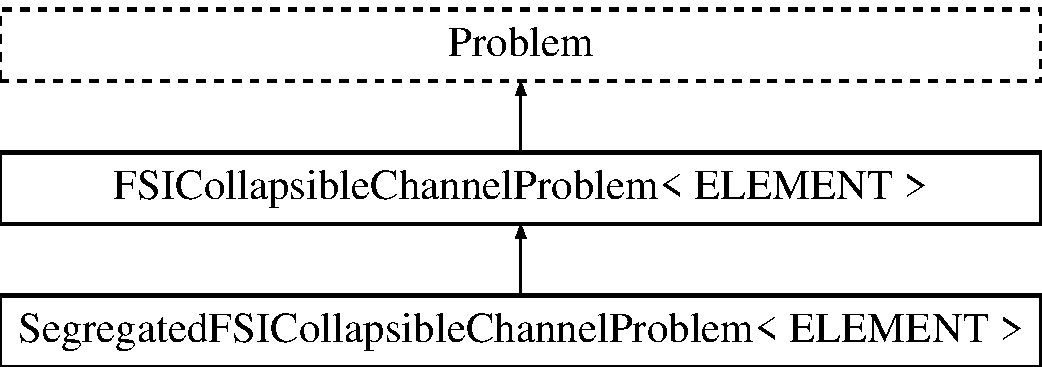
\includegraphics[height=1.014493cm]{classFSICollapsibleChannelProblem}
\end{center}
\end{figure}
\subsection*{Public Member Functions}
\begin{DoxyCompactItemize}
\item 
\hyperlink{classFSICollapsibleChannelProblem_afe14ae0d2bdfc9a15969c9bdcd6e2512}{F\+S\+I\+Collapsible\+Channel\+Problem} (const unsigned \&nup, const unsigned \&ncollapsible, const unsigned \&ndown, const unsigned \&ny, const double \&lup, const double \&lcollapsible, const double \&ldown, const double \&ly)
\begin{DoxyCompactList}\small\item\em Constructor\+: The arguments are the number of elements and the lengths of the domain. \end{DoxyCompactList}\item 
\hyperlink{classFSICollapsibleChannelProblem_abe33aaaae15ea3eb10885527a1d1ad9a}{$\sim$\+F\+S\+I\+Collapsible\+Channel\+Problem} ()
\begin{DoxyCompactList}\small\item\em Destructor (empty) \end{DoxyCompactList}\item 
\hyperlink{classoomph_1_1MacroElementNodeUpdateCollapsibleChannelMesh}{Macro\+Element\+Node\+Update\+Collapsible\+Channel\+Mesh}$<$ E\+L\+E\+M\+E\+NT $>$ $\ast$ \hyperlink{classFSICollapsibleChannelProblem_a5ea2780b4f97b65b5c122a952093e6c2}{bulk\+\_\+mesh\+\_\+pt} ()
\begin{DoxyCompactList}\small\item\em Access function for the specific bulk (fluid) mesh. \end{DoxyCompactList}\item 
\hyperlink{classoomph_1_1AlgebraicCollapsibleChannelMesh}{Algebraic\+Collapsible\+Channel\+Mesh}$<$ E\+L\+E\+M\+E\+NT $>$ $\ast$ \hyperlink{classFSICollapsibleChannelProblem_a9b461f3afef3185ea0b461714675ef8f}{bulk\+\_\+mesh\+\_\+pt} ()
\begin{DoxyCompactList}\small\item\em Access function for the specific bulk (fluid) mesh. \end{DoxyCompactList}\item 
\hyperlink{classoomph_1_1OneDLagrangianMesh}{One\+D\+Lagrangian\+Mesh}$<$ F\+S\+I\+Hermite\+Beam\+Element $>$ $\ast$ \hyperlink{classFSICollapsibleChannelProblem_ae8b71da8da82f3c52387052ce400b930}{wall\+\_\+mesh\+\_\+pt} ()
\begin{DoxyCompactList}\small\item\em Access function for the wall mesh. \end{DoxyCompactList}\item 
void \hyperlink{classFSICollapsibleChannelProblem_ad10b2d12be052c6b1bc5005dc27cd229}{actions\+\_\+before\+\_\+newton\+\_\+solve} ()
\begin{DoxyCompactList}\small\item\em Update the problem specs before solve (empty) \end{DoxyCompactList}\item 
void \hyperlink{classFSICollapsibleChannelProblem_a49780267c05f4c6ecbed11bfc6b9956b}{actions\+\_\+after\+\_\+newton\+\_\+solve} ()
\begin{DoxyCompactList}\small\item\em Update the problem after solve (empty) \end{DoxyCompactList}\item 
void \hyperlink{classFSICollapsibleChannelProblem_ace5343d2e6e6e0480d077d4f17365288}{actions\+\_\+before\+\_\+newton\+\_\+convergence\+\_\+check} ()
\begin{DoxyCompactList}\small\item\em Update before checking Newton convergence\+: Update the nodal positions in the fluid mesh in response to possible changes in the wall shape. \end{DoxyCompactList}\item 
void \hyperlink{classFSICollapsibleChannelProblem_aff5cacbc8d81f6c1beda947085496462}{doc\+\_\+solution} (Doc\+Info \&doc\+\_\+info, ofstream \&trace\+\_\+file)
\begin{DoxyCompactList}\small\item\em Doc the solution. \end{DoxyCompactList}\item 
void \hyperlink{classFSICollapsibleChannelProblem_afdd6752cb134fd09ee8830158ed557b2}{set\+\_\+initial\+\_\+condition} ()
\begin{DoxyCompactList}\small\item\em Apply initial conditions. \end{DoxyCompactList}\item 
\hyperlink{classFSICollapsibleChannelProblem_afe14ae0d2bdfc9a15969c9bdcd6e2512}{F\+S\+I\+Collapsible\+Channel\+Problem} (const unsigned \&nup, const unsigned \&ncollapsible, const unsigned \&ndown, const unsigned \&ny, const double \&lup, const double \&lcollapsible, const double \&ldown, const double \&ly)
\begin{DoxyCompactList}\small\item\em Constructor\+: The arguments are the number of elements and the lengths of the domain. \end{DoxyCompactList}\item 
\hyperlink{classFSICollapsibleChannelProblem_abe33aaaae15ea3eb10885527a1d1ad9a}{$\sim$\+F\+S\+I\+Collapsible\+Channel\+Problem} ()
\begin{DoxyCompactList}\small\item\em Destructor (empty) \end{DoxyCompactList}\item 
\hyperlink{classoomph_1_1MacroElementNodeUpdateRefineableCollapsibleChannelMesh}{Macro\+Element\+Node\+Update\+Refineable\+Collapsible\+Channel\+Mesh}$<$ E\+L\+E\+M\+E\+NT $>$ $\ast$ \hyperlink{classFSICollapsibleChannelProblem_a6c031288ea229296c10e5f41c7b3e99e}{bulk\+\_\+mesh\+\_\+pt} ()
\begin{DoxyCompactList}\small\item\em Access function for the specific bulk (fluid) mesh. \end{DoxyCompactList}\item 
\hyperlink{classoomph_1_1RefineableAlgebraicCollapsibleChannelMesh}{Refineable\+Algebraic\+Collapsible\+Channel\+Mesh}$<$ E\+L\+E\+M\+E\+NT $>$ $\ast$ \hyperlink{classFSICollapsibleChannelProblem_afa3825057e5875deda297c68eb893f74}{bulk\+\_\+mesh\+\_\+pt} ()
\begin{DoxyCompactList}\small\item\em Access function for the specific bulk (fluid) mesh. \end{DoxyCompactList}\item 
\hyperlink{classoomph_1_1OneDLagrangianMesh}{One\+D\+Lagrangian\+Mesh}$<$ F\+S\+I\+Hermite\+Beam\+Element $>$ $\ast$ \hyperlink{classFSICollapsibleChannelProblem_ae8b71da8da82f3c52387052ce400b930}{wall\+\_\+mesh\+\_\+pt} ()
\begin{DoxyCompactList}\small\item\em Access function for the wall mesh. \end{DoxyCompactList}\item 
void \hyperlink{classFSICollapsibleChannelProblem_a91b30b3d0369c178d3a79f5658644f1b}{actions\+\_\+before\+\_\+adapt} ()
\begin{DoxyCompactList}\small\item\em Actions before adapt\+: Wipe the mesh of prescribed traction elements. \end{DoxyCompactList}\item 
void \hyperlink{classFSICollapsibleChannelProblem_ae20eb7ed895e0063ade5a6d0c6f9af2f}{actions\+\_\+after\+\_\+adapt} ()
\begin{DoxyCompactList}\small\item\em Actions after adapt\+: Rebuild the mesh of prescribed traction elements. \end{DoxyCompactList}\item 
void \hyperlink{classFSICollapsibleChannelProblem_ad10b2d12be052c6b1bc5005dc27cd229}{actions\+\_\+before\+\_\+newton\+\_\+solve} ()
\begin{DoxyCompactList}\small\item\em Update the problem specs before solve (empty) \end{DoxyCompactList}\item 
void \hyperlink{classFSICollapsibleChannelProblem_a49780267c05f4c6ecbed11bfc6b9956b}{actions\+\_\+after\+\_\+newton\+\_\+solve} ()
\begin{DoxyCompactList}\small\item\em Update the problem after solve (empty) \end{DoxyCompactList}\item 
void \hyperlink{classFSICollapsibleChannelProblem_ace5343d2e6e6e0480d077d4f17365288}{actions\+\_\+before\+\_\+newton\+\_\+convergence\+\_\+check} ()
\begin{DoxyCompactList}\small\item\em Update before checking Newton convergence\+: Update the nodal positions in the fluid mesh in response to possible changes in the wall shape. \end{DoxyCompactList}\item 
void \hyperlink{classFSICollapsibleChannelProblem_aff5cacbc8d81f6c1beda947085496462}{doc\+\_\+solution} (Doc\+Info \&doc\+\_\+info, ofstream \&trace\+\_\+file)
\begin{DoxyCompactList}\small\item\em Doc the solution. \end{DoxyCompactList}\item 
void \hyperlink{classFSICollapsibleChannelProblem_afdd6752cb134fd09ee8830158ed557b2}{set\+\_\+initial\+\_\+condition} ()
\begin{DoxyCompactList}\small\item\em Apply initial conditions. \end{DoxyCompactList}\item 
\hyperlink{classFSICollapsibleChannelProblem_afe14ae0d2bdfc9a15969c9bdcd6e2512}{F\+S\+I\+Collapsible\+Channel\+Problem} (const unsigned \&nup, const unsigned \&ncollapsible, const unsigned \&ndown, const unsigned \&ny, const double \&lup, const double \&lcollapsible, const double \&ldown, const double \&ly)
\begin{DoxyCompactList}\small\item\em Constructor\+: The arguments are the number of elements and the lengths of the domain. \end{DoxyCompactList}\item 
\hyperlink{classFSICollapsibleChannelProblem_abe33aaaae15ea3eb10885527a1d1ad9a}{$\sim$\+F\+S\+I\+Collapsible\+Channel\+Problem} ()
\begin{DoxyCompactList}\small\item\em Destructor (empty) \end{DoxyCompactList}\item 
\hyperlink{classElasticCollapsibleChannelMesh}{Elastic\+Collapsible\+Channel\+Mesh}$<$ E\+L\+E\+M\+E\+NT $>$ $\ast$ \hyperlink{classFSICollapsibleChannelProblem_a90bfc02608e7fa6a69b14b6d5cfb939e}{bulk\+\_\+mesh\+\_\+pt} ()
\begin{DoxyCompactList}\small\item\em Access function for the specific bulk (fluid) mesh. \end{DoxyCompactList}\item 
\hyperlink{classoomph_1_1OneDLagrangianMesh}{One\+D\+Lagrangian\+Mesh}$<$ F\+S\+I\+Hermite\+Beam\+Element $>$ $\ast$ \hyperlink{classFSICollapsibleChannelProblem_ae8b71da8da82f3c52387052ce400b930}{wall\+\_\+mesh\+\_\+pt} ()
\begin{DoxyCompactList}\small\item\em Access function for the wall mesh. \end{DoxyCompactList}\item 
void \hyperlink{classFSICollapsibleChannelProblem_ad10b2d12be052c6b1bc5005dc27cd229}{actions\+\_\+before\+\_\+newton\+\_\+solve} ()
\begin{DoxyCompactList}\small\item\em Update the problem specs before solve (empty) \end{DoxyCompactList}\item 
void \hyperlink{classFSICollapsibleChannelProblem_a49780267c05f4c6ecbed11bfc6b9956b}{actions\+\_\+after\+\_\+newton\+\_\+solve} ()
\begin{DoxyCompactList}\small\item\em Update the problem after solve (empty) \end{DoxyCompactList}\item 
void \hyperlink{classFSICollapsibleChannelProblem_ace5343d2e6e6e0480d077d4f17365288}{actions\+\_\+before\+\_\+newton\+\_\+convergence\+\_\+check} ()
\begin{DoxyCompactList}\small\item\em Update no slip before Newton convergence check. \end{DoxyCompactList}\item 
void \hyperlink{classFSICollapsibleChannelProblem_aff5cacbc8d81f6c1beda947085496462}{doc\+\_\+solution} (Doc\+Info \&doc\+\_\+info, ofstream \&trace\+\_\+file)
\begin{DoxyCompactList}\small\item\em Doc the solution. \end{DoxyCompactList}\item 
void \hyperlink{classFSICollapsibleChannelProblem_afdd6752cb134fd09ee8830158ed557b2}{set\+\_\+initial\+\_\+condition} ()
\begin{DoxyCompactList}\small\item\em Apply initial conditions. \end{DoxyCompactList}\item 
\hyperlink{classFSICollapsibleChannelProblem_afe14ae0d2bdfc9a15969c9bdcd6e2512}{F\+S\+I\+Collapsible\+Channel\+Problem} (const unsigned \&nup, const unsigned \&ncollapsible, const unsigned \&ndown, const unsigned \&ny, const double \&lup, const double \&lcollapsible, const double \&ldown, const double \&ly)
\begin{DoxyCompactList}\small\item\em Constructor\+: The arguments are the number of elements and the lengths of the domain. \end{DoxyCompactList}\item 
\hyperlink{classFSICollapsibleChannelProblem_abe33aaaae15ea3eb10885527a1d1ad9a}{$\sim$\+F\+S\+I\+Collapsible\+Channel\+Problem} ()
\begin{DoxyCompactList}\small\item\em Destructor (empty) \end{DoxyCompactList}\item 
\hyperlink{classElasticRefineableCollapsibleChannelMesh}{Elastic\+Refineable\+Collapsible\+Channel\+Mesh}$<$ E\+L\+E\+M\+E\+NT $>$ $\ast$ \hyperlink{classFSICollapsibleChannelProblem_ac08de7f582e4e2d7e6953edd15707d89}{bulk\+\_\+mesh\+\_\+pt} ()
\begin{DoxyCompactList}\small\item\em Access function for the specific bulk (fluid) mesh. \end{DoxyCompactList}\item 
\hyperlink{classoomph_1_1OneDLagrangianMesh}{One\+D\+Lagrangian\+Mesh}$<$ F\+S\+I\+Hermite\+Beam\+Element $>$ $\ast$ \hyperlink{classFSICollapsibleChannelProblem_ae8b71da8da82f3c52387052ce400b930}{wall\+\_\+mesh\+\_\+pt} ()
\begin{DoxyCompactList}\small\item\em Access function for the wall mesh. \end{DoxyCompactList}\item 
void \hyperlink{classFSICollapsibleChannelProblem_a91b30b3d0369c178d3a79f5658644f1b}{actions\+\_\+before\+\_\+adapt} ()
\begin{DoxyCompactList}\small\item\em Actions before adapt\+: Wipe the mesh of prescribed traction elements. \end{DoxyCompactList}\item 
void \hyperlink{classFSICollapsibleChannelProblem_ae20eb7ed895e0063ade5a6d0c6f9af2f}{actions\+\_\+after\+\_\+adapt} ()
\item 
void \hyperlink{classFSICollapsibleChannelProblem_ad10b2d12be052c6b1bc5005dc27cd229}{actions\+\_\+before\+\_\+newton\+\_\+solve} ()
\begin{DoxyCompactList}\small\item\em Update the problem specs before solve (empty) \end{DoxyCompactList}\item 
void \hyperlink{classFSICollapsibleChannelProblem_a49780267c05f4c6ecbed11bfc6b9956b}{actions\+\_\+after\+\_\+newton\+\_\+solve} ()
\begin{DoxyCompactList}\small\item\em Update the problem after solve (empty) \end{DoxyCompactList}\item 
void \hyperlink{classFSICollapsibleChannelProblem_ace5343d2e6e6e0480d077d4f17365288}{actions\+\_\+before\+\_\+newton\+\_\+convergence\+\_\+check} ()
\begin{DoxyCompactList}\small\item\em Update no slip before Newton convergence check. \end{DoxyCompactList}\item 
void \hyperlink{classFSICollapsibleChannelProblem_aff5cacbc8d81f6c1beda947085496462}{doc\+\_\+solution} (Doc\+Info \&doc\+\_\+info, ofstream \&trace\+\_\+file)
\begin{DoxyCompactList}\small\item\em Doc the solution. \end{DoxyCompactList}\item 
void \hyperlink{classFSICollapsibleChannelProblem_afdd6752cb134fd09ee8830158ed557b2}{set\+\_\+initial\+\_\+condition} ()
\begin{DoxyCompactList}\small\item\em Apply initial conditions. \end{DoxyCompactList}\end{DoxyCompactItemize}
\subsection*{Private Member Functions}
\begin{DoxyCompactItemize}
\item 
void \hyperlink{classFSICollapsibleChannelProblem_af7352e5fd5ea8965adbc9505749442a3}{create\+\_\+traction\+\_\+elements} (const unsigned \&b, Mesh $\ast$const \&\hyperlink{classFSICollapsibleChannelProblem_a5ea2780b4f97b65b5c122a952093e6c2}{bulk\+\_\+mesh\+\_\+pt}, Mesh $\ast$const \&traction\+\_\+mesh\+\_\+pt)
\begin{DoxyCompactList}\small\item\em Create the prescribed traction elements on boundary b. \end{DoxyCompactList}\item 
void \hyperlink{classFSICollapsibleChannelProblem_af7352e5fd5ea8965adbc9505749442a3}{create\+\_\+traction\+\_\+elements} (const unsigned \&b, Mesh $\ast$const \&\hyperlink{classFSICollapsibleChannelProblem_a5ea2780b4f97b65b5c122a952093e6c2}{bulk\+\_\+mesh\+\_\+pt}, Mesh $\ast$const \&traction\+\_\+mesh\+\_\+pt)
\begin{DoxyCompactList}\small\item\em Create the prescribed traction elements on boundary b. \end{DoxyCompactList}\item 
void \hyperlink{classFSICollapsibleChannelProblem_af1848415423aa824b91357922905a18f}{delete\+\_\+traction\+\_\+elements} (Mesh $\ast$const \&traction\+\_\+mesh\+\_\+pt)
\begin{DoxyCompactList}\small\item\em Delete prescribed traction elements from the surface mesh. \end{DoxyCompactList}\item 
void \hyperlink{classFSICollapsibleChannelProblem_af7352e5fd5ea8965adbc9505749442a3}{create\+\_\+traction\+\_\+elements} (const unsigned \&b, Mesh $\ast$const \&\hyperlink{classFSICollapsibleChannelProblem_a5ea2780b4f97b65b5c122a952093e6c2}{bulk\+\_\+mesh\+\_\+pt}, Mesh $\ast$const \&traction\+\_\+mesh\+\_\+pt)
\begin{DoxyCompactList}\small\item\em Create the prescribed traction elements on boundary b. \end{DoxyCompactList}\item 
void \hyperlink{classFSICollapsibleChannelProblem_af1848415423aa824b91357922905a18f}{delete\+\_\+traction\+\_\+elements} (Mesh $\ast$const \&traction\+\_\+mesh\+\_\+pt)
\begin{DoxyCompactList}\small\item\em Delete prescribed traction elements from the surface mesh. \end{DoxyCompactList}\item 
void \hyperlink{classFSICollapsibleChannelProblem_a328465bc567702963e06c07f5550f80a}{create\+\_\+lagrange\+\_\+multiplier\+\_\+elements} ()
\begin{DoxyCompactList}\small\item\em Create elements that enforce prescribed boundary motion by Lagrange multipliers. \end{DoxyCompactList}\item 
void \hyperlink{classFSICollapsibleChannelProblem_ab853c978c8e94505cd36781569b1dbf1}{delete\+\_\+lagrange\+\_\+multiplier\+\_\+elements} ()
\item 
void \hyperlink{classFSICollapsibleChannelProblem_af7352e5fd5ea8965adbc9505749442a3}{create\+\_\+traction\+\_\+elements} (const unsigned \&b, Mesh $\ast$const \&\hyperlink{classFSICollapsibleChannelProblem_a5ea2780b4f97b65b5c122a952093e6c2}{bulk\+\_\+mesh\+\_\+pt}, Mesh $\ast$const \&traction\+\_\+mesh\+\_\+pt)
\begin{DoxyCompactList}\small\item\em Create the prescribed traction elements on boundary b. \end{DoxyCompactList}\item 
void \hyperlink{classFSICollapsibleChannelProblem_af1848415423aa824b91357922905a18f}{delete\+\_\+traction\+\_\+elements} (Mesh $\ast$const \&traction\+\_\+mesh\+\_\+pt)
\begin{DoxyCompactList}\small\item\em Delete prescribed traction elements from the surface mesh. \end{DoxyCompactList}\item 
void \hyperlink{classFSICollapsibleChannelProblem_a328465bc567702963e06c07f5550f80a}{create\+\_\+lagrange\+\_\+multiplier\+\_\+elements} ()
\begin{DoxyCompactList}\small\item\em Create elements that enforce prescribed boundary motion by Lagrange multiplilers. \end{DoxyCompactList}\item 
void \hyperlink{classFSICollapsibleChannelProblem_ab853c978c8e94505cd36781569b1dbf1}{delete\+\_\+lagrange\+\_\+multiplier\+\_\+elements} ()
\end{DoxyCompactItemize}
\subsection*{Private Attributes}
\begin{DoxyCompactItemize}
\item 
unsigned \hyperlink{classFSICollapsibleChannelProblem_a22a5ea767bf0c437b78ed4e37b7a4818}{Nup}
\begin{DoxyCompactList}\small\item\em Number of elements in the x direction in the upstream part of the channel. \end{DoxyCompactList}\item 
unsigned \hyperlink{classFSICollapsibleChannelProblem_a3fb9656feb1c32045f4fdbd74f91258f}{Ncollapsible}
\begin{DoxyCompactList}\small\item\em Number of elements in the x direction in the collapsible part of the channel. \end{DoxyCompactList}\item 
unsigned \hyperlink{classFSICollapsibleChannelProblem_a64c0aa974b39527ef22e352a4f22b156}{Ndown}
\begin{DoxyCompactList}\small\item\em Number of elements in the x direction in the downstream part of the channel. \end{DoxyCompactList}\item 
unsigned \hyperlink{classFSICollapsibleChannelProblem_a536804b714fd0033f3028ff1c6032918}{Ny}
\begin{DoxyCompactList}\small\item\em Number of elements across the channel. \end{DoxyCompactList}\item 
double \hyperlink{classFSICollapsibleChannelProblem_a7b8288e57097875d247bda6201b1bfcf}{Lup}
\begin{DoxyCompactList}\small\item\em x-\/length in the upstream part of the channel \end{DoxyCompactList}\item 
double \hyperlink{classFSICollapsibleChannelProblem_ae6ce3834d06f0fb75db945a782ff0108}{Lcollapsible}
\begin{DoxyCompactList}\small\item\em x-\/length in the collapsible part of the channel \end{DoxyCompactList}\item 
double \hyperlink{classFSICollapsibleChannelProblem_a0964686847cc64f2a77a866187aec626}{Ldown}
\begin{DoxyCompactList}\small\item\em x-\/length in the downstream part of the channel \end{DoxyCompactList}\item 
double \hyperlink{classFSICollapsibleChannelProblem_adb381270408cea69b7290ff2aeb5928f}{Ly}
\begin{DoxyCompactList}\small\item\em Transverse length. \end{DoxyCompactList}\item 
\hyperlink{classoomph_1_1MacroElementNodeUpdateCollapsibleChannelMesh}{Macro\+Element\+Node\+Update\+Collapsible\+Channel\+Mesh}$<$ E\+L\+E\+M\+E\+NT $>$ $\ast$ \hyperlink{classFSICollapsibleChannelProblem_ab2eb47a9ed4ce8adb3b11ac316644cde}{Bulk\+\_\+mesh\+\_\+pt}
\begin{DoxyCompactList}\small\item\em Pointer to the \char`\"{}bulk\char`\"{} mesh. \end{DoxyCompactList}\item 
\hyperlink{classoomph_1_1AlgebraicCollapsibleChannelMesh}{Algebraic\+Collapsible\+Channel\+Mesh}$<$ E\+L\+E\+M\+E\+NT $>$ $\ast$ \hyperlink{classFSICollapsibleChannelProblem_a74c09286f4ad4242c37b6ea16c069fae}{Bulk\+\_\+mesh\+\_\+pt}
\begin{DoxyCompactList}\small\item\em Pointer to the \char`\"{}bulk\char`\"{} mesh. \end{DoxyCompactList}\item 
Mesh $\ast$ \hyperlink{classFSICollapsibleChannelProblem_a0594bd63457b032bcf2a1b6bba534c7e}{Applied\+\_\+fluid\+\_\+traction\+\_\+mesh\+\_\+pt}
\begin{DoxyCompactList}\small\item\em Pointer to the \char`\"{}surface\char`\"{} mesh that applies the traction at the inflow. \end{DoxyCompactList}\item 
\hyperlink{classoomph_1_1OneDLagrangianMesh}{One\+D\+Lagrangian\+Mesh}$<$ F\+S\+I\+Hermite\+Beam\+Element $>$ $\ast$ \hyperlink{classFSICollapsibleChannelProblem_a2699abcfe8de6b73bbef098e0f0dc1db}{Wall\+\_\+mesh\+\_\+pt}
\begin{DoxyCompactList}\small\item\em Pointer to the \char`\"{}wall\char`\"{} mesh. \end{DoxyCompactList}\item 
Node $\ast$ \hyperlink{classFSICollapsibleChannelProblem_a0e5fd455e2956e74485678d4357b4869}{Left\+\_\+node\+\_\+pt}
\begin{DoxyCompactList}\small\item\em Pointer to the left control node. \end{DoxyCompactList}\item 
Node $\ast$ \hyperlink{classFSICollapsibleChannelProblem_a194e116e377045afba000fba80a46fa8}{Right\+\_\+node\+\_\+pt}
\begin{DoxyCompactList}\small\item\em Pointer to right control node. \end{DoxyCompactList}\item 
Node $\ast$ \hyperlink{classFSICollapsibleChannelProblem_ad840e3bf0ee356ac054d9bcab97471d9}{Wall\+\_\+node\+\_\+pt}
\begin{DoxyCompactList}\small\item\em Pointer to control node on the wall. \end{DoxyCompactList}\item 
\hyperlink{classoomph_1_1MacroElementNodeUpdateRefineableCollapsibleChannelMesh}{Macro\+Element\+Node\+Update\+Refineable\+Collapsible\+Channel\+Mesh}$<$ E\+L\+E\+M\+E\+NT $>$ $\ast$ \hyperlink{classFSICollapsibleChannelProblem_a211bcc5fb6076133f46d63bfd827dd3f}{Bulk\+\_\+mesh\+\_\+pt}
\begin{DoxyCompactList}\small\item\em Pointer to the \char`\"{}bulk\char`\"{} mesh. \end{DoxyCompactList}\item 
\hyperlink{classoomph_1_1RefineableAlgebraicCollapsibleChannelMesh}{Refineable\+Algebraic\+Collapsible\+Channel\+Mesh}$<$ E\+L\+E\+M\+E\+NT $>$ $\ast$ \hyperlink{classFSICollapsibleChannelProblem_aa0da71e3534daa79c0c4c2e6dbc6338c}{Bulk\+\_\+mesh\+\_\+pt}
\begin{DoxyCompactList}\small\item\em Pointer to the \char`\"{}bulk\char`\"{} mesh. \end{DoxyCompactList}\item 
\hyperlink{classElasticCollapsibleChannelMesh}{Elastic\+Collapsible\+Channel\+Mesh}$<$ E\+L\+E\+M\+E\+NT $>$ $\ast$ \hyperlink{classFSICollapsibleChannelProblem_a73b35b23f07b5f79e288064c2e62e1ac}{Bulk\+\_\+mesh\+\_\+pt}
\begin{DoxyCompactList}\small\item\em Pointer to the \char`\"{}bulk\char`\"{} mesh. \end{DoxyCompactList}\item 
Solid\+Mesh $\ast$ \hyperlink{classFSICollapsibleChannelProblem_a3a5aa5a00fbecec4bede0aee9af6b338}{Lagrange\+\_\+multiplier\+\_\+mesh\+\_\+pt}
\begin{DoxyCompactList}\small\item\em Pointers to mesh of Lagrange multiplier elements. \end{DoxyCompactList}\item 
Mesh\+As\+Geom\+Object $\ast$ \hyperlink{classFSICollapsibleChannelProblem_a884256a97060121c507ab9673f0ccef6}{Wall\+\_\+geom\+\_\+object\+\_\+pt}
\begin{DoxyCompactList}\small\item\em Geometric object incarnation of the wall mesh. \end{DoxyCompactList}\item 
Constitutive\+Law $\ast$ \hyperlink{classFSICollapsibleChannelProblem_a49de3f64c8f375c2709a2d0f5193cef3}{Constitutive\+\_\+law\+\_\+pt}
\begin{DoxyCompactList}\small\item\em Constitutive law used to determine the mesh deformation. \end{DoxyCompactList}\item 
\hyperlink{classElasticRefineableCollapsibleChannelMesh}{Elastic\+Refineable\+Collapsible\+Channel\+Mesh}$<$ E\+L\+E\+M\+E\+NT $>$ $\ast$ \hyperlink{classFSICollapsibleChannelProblem_ac7c827b880d5499b8c3c4c3c37d6a3c9}{Bulk\+\_\+mesh\+\_\+pt}
\begin{DoxyCompactList}\small\item\em Pointer to the \char`\"{}bulk\char`\"{} mesh. \end{DoxyCompactList}\end{DoxyCompactItemize}


\subsection{Detailed Description}
\subsubsection*{template$<$class E\+L\+E\+M\+E\+NT$>$\newline
class F\+S\+I\+Collapsible\+Channel\+Problem$<$ E\+L\+E\+M\+E\+N\+T $>$}

Problem class. 

Definition at line 237 of file fsi\+\_\+collapsible\+\_\+channel.\+cc.



\subsection{Constructor \& Destructor Documentation}
\mbox{\Hypertarget{classFSICollapsibleChannelProblem_afe14ae0d2bdfc9a15969c9bdcd6e2512}\label{classFSICollapsibleChannelProblem_afe14ae0d2bdfc9a15969c9bdcd6e2512}} 
\index{F\+S\+I\+Collapsible\+Channel\+Problem@{F\+S\+I\+Collapsible\+Channel\+Problem}!F\+S\+I\+Collapsible\+Channel\+Problem@{F\+S\+I\+Collapsible\+Channel\+Problem}}
\index{F\+S\+I\+Collapsible\+Channel\+Problem@{F\+S\+I\+Collapsible\+Channel\+Problem}!F\+S\+I\+Collapsible\+Channel\+Problem@{F\+S\+I\+Collapsible\+Channel\+Problem}}
\subsubsection{\texorpdfstring{F\+S\+I\+Collapsible\+Channel\+Problem()}{FSICollapsibleChannelProblem()}\hspace{0.1cm}{\footnotesize\ttfamily [1/4]}}
{\footnotesize\ttfamily template$<$class E\+L\+E\+M\+E\+NT $>$ \\
\hyperlink{classFSICollapsibleChannelProblem}{F\+S\+I\+Collapsible\+Channel\+Problem}$<$ E\+L\+E\+M\+E\+NT $>$\+::\hyperlink{classFSICollapsibleChannelProblem}{F\+S\+I\+Collapsible\+Channel\+Problem} (\begin{DoxyParamCaption}\item[{const unsigned \&}]{nup,  }\item[{const unsigned \&}]{ncollapsible,  }\item[{const unsigned \&}]{ndown,  }\item[{const unsigned \&}]{ny,  }\item[{const double \&}]{lup,  }\item[{const double \&}]{lcollapsible,  }\item[{const double \&}]{ldown,  }\item[{const double \&}]{ly }\end{DoxyParamCaption})}



Constructor\+: The arguments are the number of elements and the lengths of the domain. 

Constructor for the collapsible channel problem. 

Definition at line 382 of file fsi\+\_\+collapsible\+\_\+channel.\+cc.



References oomph\+::\+Collapsible\+Channel\+Mesh$<$ E\+L\+E\+M\+E\+N\+T $>$\+::bl\+\_\+squash\+\_\+fct\+\_\+pt(), Global\+\_\+\+Physical\+\_\+\+Variables\+::H, Global\+\_\+\+Physical\+\_\+\+Variables\+::load(), Global\+\_\+\+Physical\+\_\+\+Variables\+::prescribed\+\_\+traction(), Global\+\_\+\+Physical\+\_\+\+Variables\+::Q, Global\+\_\+\+Physical\+\_\+\+Variables\+::\+Re, Global\+\_\+\+Physical\+\_\+\+Variables\+::\+Re\+St, Global\+\_\+\+Physical\+\_\+\+Variables\+::\+Sigma0, and B\+L\+\_\+\+Squash\+::squash\+\_\+fct().

\mbox{\Hypertarget{classFSICollapsibleChannelProblem_abe33aaaae15ea3eb10885527a1d1ad9a}\label{classFSICollapsibleChannelProblem_abe33aaaae15ea3eb10885527a1d1ad9a}} 
\index{F\+S\+I\+Collapsible\+Channel\+Problem@{F\+S\+I\+Collapsible\+Channel\+Problem}!````~F\+S\+I\+Collapsible\+Channel\+Problem@{$\sim$\+F\+S\+I\+Collapsible\+Channel\+Problem}}
\index{````~F\+S\+I\+Collapsible\+Channel\+Problem@{$\sim$\+F\+S\+I\+Collapsible\+Channel\+Problem}!F\+S\+I\+Collapsible\+Channel\+Problem@{F\+S\+I\+Collapsible\+Channel\+Problem}}
\subsubsection{\texorpdfstring{$\sim$\+F\+S\+I\+Collapsible\+Channel\+Problem()}{~FSICollapsibleChannelProblem()}\hspace{0.1cm}{\footnotesize\ttfamily [1/4]}}
{\footnotesize\ttfamily template$<$class E\+L\+E\+M\+E\+NT $>$ \\
\hyperlink{classFSICollapsibleChannelProblem}{F\+S\+I\+Collapsible\+Channel\+Problem}$<$ E\+L\+E\+M\+E\+NT $>$\+::$\sim$\hyperlink{classFSICollapsibleChannelProblem}{F\+S\+I\+Collapsible\+Channel\+Problem} (\begin{DoxyParamCaption}{ }\end{DoxyParamCaption})\hspace{0.3cm}{\ttfamily [inline]}}



Destructor (empty) 



Definition at line 254 of file fsi\+\_\+collapsible\+\_\+channel.\+cc.

\mbox{\Hypertarget{classFSICollapsibleChannelProblem_afe14ae0d2bdfc9a15969c9bdcd6e2512}\label{classFSICollapsibleChannelProblem_afe14ae0d2bdfc9a15969c9bdcd6e2512}} 
\index{F\+S\+I\+Collapsible\+Channel\+Problem@{F\+S\+I\+Collapsible\+Channel\+Problem}!F\+S\+I\+Collapsible\+Channel\+Problem@{F\+S\+I\+Collapsible\+Channel\+Problem}}
\index{F\+S\+I\+Collapsible\+Channel\+Problem@{F\+S\+I\+Collapsible\+Channel\+Problem}!F\+S\+I\+Collapsible\+Channel\+Problem@{F\+S\+I\+Collapsible\+Channel\+Problem}}
\subsubsection{\texorpdfstring{F\+S\+I\+Collapsible\+Channel\+Problem()}{FSICollapsibleChannelProblem()}\hspace{0.1cm}{\footnotesize\ttfamily [2/4]}}
{\footnotesize\ttfamily template$<$class E\+L\+E\+M\+E\+NT $>$ \\
\hyperlink{classFSICollapsibleChannelProblem}{F\+S\+I\+Collapsible\+Channel\+Problem}$<$ E\+L\+E\+M\+E\+NT $>$\+::\hyperlink{classFSICollapsibleChannelProblem}{F\+S\+I\+Collapsible\+Channel\+Problem} (\begin{DoxyParamCaption}\item[{const unsigned \&}]{nup,  }\item[{const unsigned \&}]{ncollapsible,  }\item[{const unsigned \&}]{ndown,  }\item[{const unsigned \&}]{ny,  }\item[{const double \&}]{lup,  }\item[{const double \&}]{lcollapsible,  }\item[{const double \&}]{ldown,  }\item[{const double \&}]{ly }\end{DoxyParamCaption})}



Constructor\+: The arguments are the number of elements and the lengths of the domain. 

\mbox{\Hypertarget{classFSICollapsibleChannelProblem_abe33aaaae15ea3eb10885527a1d1ad9a}\label{classFSICollapsibleChannelProblem_abe33aaaae15ea3eb10885527a1d1ad9a}} 
\index{F\+S\+I\+Collapsible\+Channel\+Problem@{F\+S\+I\+Collapsible\+Channel\+Problem}!````~F\+S\+I\+Collapsible\+Channel\+Problem@{$\sim$\+F\+S\+I\+Collapsible\+Channel\+Problem}}
\index{````~F\+S\+I\+Collapsible\+Channel\+Problem@{$\sim$\+F\+S\+I\+Collapsible\+Channel\+Problem}!F\+S\+I\+Collapsible\+Channel\+Problem@{F\+S\+I\+Collapsible\+Channel\+Problem}}
\subsubsection{\texorpdfstring{$\sim$\+F\+S\+I\+Collapsible\+Channel\+Problem()}{~FSICollapsibleChannelProblem()}\hspace{0.1cm}{\footnotesize\ttfamily [2/4]}}
{\footnotesize\ttfamily template$<$class E\+L\+E\+M\+E\+NT $>$ \\
\hyperlink{classFSICollapsibleChannelProblem}{F\+S\+I\+Collapsible\+Channel\+Problem}$<$ E\+L\+E\+M\+E\+NT $>$\+::$\sim$\hyperlink{classFSICollapsibleChannelProblem}{F\+S\+I\+Collapsible\+Channel\+Problem} (\begin{DoxyParamCaption}{ }\end{DoxyParamCaption})\hspace{0.3cm}{\ttfamily [inline]}}



Destructor (empty) 



Definition at line 253 of file fsi\+\_\+collapsible\+\_\+channel\+\_\+adapt.\+cc.

\mbox{\Hypertarget{classFSICollapsibleChannelProblem_afe14ae0d2bdfc9a15969c9bdcd6e2512}\label{classFSICollapsibleChannelProblem_afe14ae0d2bdfc9a15969c9bdcd6e2512}} 
\index{F\+S\+I\+Collapsible\+Channel\+Problem@{F\+S\+I\+Collapsible\+Channel\+Problem}!F\+S\+I\+Collapsible\+Channel\+Problem@{F\+S\+I\+Collapsible\+Channel\+Problem}}
\index{F\+S\+I\+Collapsible\+Channel\+Problem@{F\+S\+I\+Collapsible\+Channel\+Problem}!F\+S\+I\+Collapsible\+Channel\+Problem@{F\+S\+I\+Collapsible\+Channel\+Problem}}
\subsubsection{\texorpdfstring{F\+S\+I\+Collapsible\+Channel\+Problem()}{FSICollapsibleChannelProblem()}\hspace{0.1cm}{\footnotesize\ttfamily [3/4]}}
{\footnotesize\ttfamily template$<$class E\+L\+E\+M\+E\+NT $>$ \\
\hyperlink{classFSICollapsibleChannelProblem}{F\+S\+I\+Collapsible\+Channel\+Problem}$<$ E\+L\+E\+M\+E\+NT $>$\+::\hyperlink{classFSICollapsibleChannelProblem}{F\+S\+I\+Collapsible\+Channel\+Problem} (\begin{DoxyParamCaption}\item[{const unsigned \&}]{nup,  }\item[{const unsigned \&}]{ncollapsible,  }\item[{const unsigned \&}]{ndown,  }\item[{const unsigned \&}]{ny,  }\item[{const double \&}]{lup,  }\item[{const double \&}]{lcollapsible,  }\item[{const double \&}]{ldown,  }\item[{const double \&}]{ly }\end{DoxyParamCaption})}



Constructor\+: The arguments are the number of elements and the lengths of the domain. 

\mbox{\Hypertarget{classFSICollapsibleChannelProblem_abe33aaaae15ea3eb10885527a1d1ad9a}\label{classFSICollapsibleChannelProblem_abe33aaaae15ea3eb10885527a1d1ad9a}} 
\index{F\+S\+I\+Collapsible\+Channel\+Problem@{F\+S\+I\+Collapsible\+Channel\+Problem}!````~F\+S\+I\+Collapsible\+Channel\+Problem@{$\sim$\+F\+S\+I\+Collapsible\+Channel\+Problem}}
\index{````~F\+S\+I\+Collapsible\+Channel\+Problem@{$\sim$\+F\+S\+I\+Collapsible\+Channel\+Problem}!F\+S\+I\+Collapsible\+Channel\+Problem@{F\+S\+I\+Collapsible\+Channel\+Problem}}
\subsubsection{\texorpdfstring{$\sim$\+F\+S\+I\+Collapsible\+Channel\+Problem()}{~FSICollapsibleChannelProblem()}\hspace{0.1cm}{\footnotesize\ttfamily [3/4]}}
{\footnotesize\ttfamily template$<$class E\+L\+E\+M\+E\+NT $>$ \\
\hyperlink{classFSICollapsibleChannelProblem}{F\+S\+I\+Collapsible\+Channel\+Problem}$<$ E\+L\+E\+M\+E\+NT $>$\+::$\sim$\hyperlink{classFSICollapsibleChannelProblem}{F\+S\+I\+Collapsible\+Channel\+Problem} (\begin{DoxyParamCaption}{ }\end{DoxyParamCaption})\hspace{0.3cm}{\ttfamily [inline]}}



Destructor (empty) 



Definition at line 299 of file fsi\+\_\+pseudo\+\_\+solid\+\_\+collapsible\+\_\+channel.\+cc.

\mbox{\Hypertarget{classFSICollapsibleChannelProblem_afe14ae0d2bdfc9a15969c9bdcd6e2512}\label{classFSICollapsibleChannelProblem_afe14ae0d2bdfc9a15969c9bdcd6e2512}} 
\index{F\+S\+I\+Collapsible\+Channel\+Problem@{F\+S\+I\+Collapsible\+Channel\+Problem}!F\+S\+I\+Collapsible\+Channel\+Problem@{F\+S\+I\+Collapsible\+Channel\+Problem}}
\index{F\+S\+I\+Collapsible\+Channel\+Problem@{F\+S\+I\+Collapsible\+Channel\+Problem}!F\+S\+I\+Collapsible\+Channel\+Problem@{F\+S\+I\+Collapsible\+Channel\+Problem}}
\subsubsection{\texorpdfstring{F\+S\+I\+Collapsible\+Channel\+Problem()}{FSICollapsibleChannelProblem()}\hspace{0.1cm}{\footnotesize\ttfamily [4/4]}}
{\footnotesize\ttfamily template$<$class E\+L\+E\+M\+E\+NT $>$ \\
\hyperlink{classFSICollapsibleChannelProblem}{F\+S\+I\+Collapsible\+Channel\+Problem}$<$ E\+L\+E\+M\+E\+NT $>$\+::\hyperlink{classFSICollapsibleChannelProblem}{F\+S\+I\+Collapsible\+Channel\+Problem} (\begin{DoxyParamCaption}\item[{const unsigned \&}]{nup,  }\item[{const unsigned \&}]{ncollapsible,  }\item[{const unsigned \&}]{ndown,  }\item[{const unsigned \&}]{ny,  }\item[{const double \&}]{lup,  }\item[{const double \&}]{lcollapsible,  }\item[{const double \&}]{ldown,  }\item[{const double \&}]{ly }\end{DoxyParamCaption})}



Constructor\+: The arguments are the number of elements and the lengths of the domain. 

\mbox{\Hypertarget{classFSICollapsibleChannelProblem_abe33aaaae15ea3eb10885527a1d1ad9a}\label{classFSICollapsibleChannelProblem_abe33aaaae15ea3eb10885527a1d1ad9a}} 
\index{F\+S\+I\+Collapsible\+Channel\+Problem@{F\+S\+I\+Collapsible\+Channel\+Problem}!````~F\+S\+I\+Collapsible\+Channel\+Problem@{$\sim$\+F\+S\+I\+Collapsible\+Channel\+Problem}}
\index{````~F\+S\+I\+Collapsible\+Channel\+Problem@{$\sim$\+F\+S\+I\+Collapsible\+Channel\+Problem}!F\+S\+I\+Collapsible\+Channel\+Problem@{F\+S\+I\+Collapsible\+Channel\+Problem}}
\subsubsection{\texorpdfstring{$\sim$\+F\+S\+I\+Collapsible\+Channel\+Problem()}{~FSICollapsibleChannelProblem()}\hspace{0.1cm}{\footnotesize\ttfamily [4/4]}}
{\footnotesize\ttfamily template$<$class E\+L\+E\+M\+E\+NT $>$ \\
\hyperlink{classFSICollapsibleChannelProblem}{F\+S\+I\+Collapsible\+Channel\+Problem}$<$ E\+L\+E\+M\+E\+NT $>$\+::$\sim$\hyperlink{classFSICollapsibleChannelProblem}{F\+S\+I\+Collapsible\+Channel\+Problem} (\begin{DoxyParamCaption}{ }\end{DoxyParamCaption})\hspace{0.3cm}{\ttfamily [inline]}}



Destructor (empty) 



Definition at line 304 of file fsi\+\_\+pseudo\+\_\+solid\+\_\+collapsible\+\_\+channel\+\_\+adapt.\+cc.



\subsection{Member Function Documentation}
\mbox{\Hypertarget{classFSICollapsibleChannelProblem_ae20eb7ed895e0063ade5a6d0c6f9af2f}\label{classFSICollapsibleChannelProblem_ae20eb7ed895e0063ade5a6d0c6f9af2f}} 
\index{F\+S\+I\+Collapsible\+Channel\+Problem@{F\+S\+I\+Collapsible\+Channel\+Problem}!actions\+\_\+after\+\_\+adapt@{actions\+\_\+after\+\_\+adapt}}
\index{actions\+\_\+after\+\_\+adapt@{actions\+\_\+after\+\_\+adapt}!F\+S\+I\+Collapsible\+Channel\+Problem@{F\+S\+I\+Collapsible\+Channel\+Problem}}
\subsubsection{\texorpdfstring{actions\+\_\+after\+\_\+adapt()}{actions\_after\_adapt()}\hspace{0.1cm}{\footnotesize\ttfamily [1/2]}}
{\footnotesize\ttfamily template$<$class E\+L\+E\+M\+E\+NT $>$ \\
void \hyperlink{classFSICollapsibleChannelProblem}{F\+S\+I\+Collapsible\+Channel\+Problem}$<$ E\+L\+E\+M\+E\+NT $>$\+::actions\+\_\+after\+\_\+adapt (\begin{DoxyParamCaption}{ }\end{DoxyParamCaption})}



Actions after adapt\+: Rebuild the mesh of prescribed traction elements. 

Actions after adapt\+: Rebuild the mesh of prescribed traction elements and reset F\+SI 

Definition at line 901 of file fsi\+\_\+collapsible\+\_\+channel\+\_\+adapt.\+cc.



References Global\+\_\+\+Physical\+\_\+\+Variables\+::prescribed\+\_\+traction().

\mbox{\Hypertarget{classFSICollapsibleChannelProblem_ae20eb7ed895e0063ade5a6d0c6f9af2f}\label{classFSICollapsibleChannelProblem_ae20eb7ed895e0063ade5a6d0c6f9af2f}} 
\index{F\+S\+I\+Collapsible\+Channel\+Problem@{F\+S\+I\+Collapsible\+Channel\+Problem}!actions\+\_\+after\+\_\+adapt@{actions\+\_\+after\+\_\+adapt}}
\index{actions\+\_\+after\+\_\+adapt@{actions\+\_\+after\+\_\+adapt}!F\+S\+I\+Collapsible\+Channel\+Problem@{F\+S\+I\+Collapsible\+Channel\+Problem}}
\subsubsection{\texorpdfstring{actions\+\_\+after\+\_\+adapt()}{actions\_after\_adapt()}\hspace{0.1cm}{\footnotesize\ttfamily [2/2]}}
{\footnotesize\ttfamily template$<$class E\+L\+E\+M\+E\+NT $>$ \\
void \hyperlink{classFSICollapsibleChannelProblem}{F\+S\+I\+Collapsible\+Channel\+Problem}$<$ E\+L\+E\+M\+E\+NT $>$\+::actions\+\_\+after\+\_\+adapt (\begin{DoxyParamCaption}{ }\end{DoxyParamCaption})}

Actions after adapt\+: Rebuild the mesh of prescribed traction elements and reset F\+SI \mbox{\Hypertarget{classFSICollapsibleChannelProblem_a49780267c05f4c6ecbed11bfc6b9956b}\label{classFSICollapsibleChannelProblem_a49780267c05f4c6ecbed11bfc6b9956b}} 
\index{F\+S\+I\+Collapsible\+Channel\+Problem@{F\+S\+I\+Collapsible\+Channel\+Problem}!actions\+\_\+after\+\_\+newton\+\_\+solve@{actions\+\_\+after\+\_\+newton\+\_\+solve}}
\index{actions\+\_\+after\+\_\+newton\+\_\+solve@{actions\+\_\+after\+\_\+newton\+\_\+solve}!F\+S\+I\+Collapsible\+Channel\+Problem@{F\+S\+I\+Collapsible\+Channel\+Problem}}
\subsubsection{\texorpdfstring{actions\+\_\+after\+\_\+newton\+\_\+solve()}{actions\_after\_newton\_solve()}\hspace{0.1cm}{\footnotesize\ttfamily [1/4]}}
{\footnotesize\ttfamily template$<$class E\+L\+E\+M\+E\+NT $>$ \\
void \hyperlink{classFSICollapsibleChannelProblem}{F\+S\+I\+Collapsible\+Channel\+Problem}$<$ E\+L\+E\+M\+E\+NT $>$\+::actions\+\_\+after\+\_\+newton\+\_\+solve (\begin{DoxyParamCaption}{ }\end{DoxyParamCaption})\hspace{0.3cm}{\ttfamily [inline]}}



Update the problem after solve (empty) 



Definition at line 296 of file fsi\+\_\+collapsible\+\_\+channel.\+cc.

\mbox{\Hypertarget{classFSICollapsibleChannelProblem_a49780267c05f4c6ecbed11bfc6b9956b}\label{classFSICollapsibleChannelProblem_a49780267c05f4c6ecbed11bfc6b9956b}} 
\index{F\+S\+I\+Collapsible\+Channel\+Problem@{F\+S\+I\+Collapsible\+Channel\+Problem}!actions\+\_\+after\+\_\+newton\+\_\+solve@{actions\+\_\+after\+\_\+newton\+\_\+solve}}
\index{actions\+\_\+after\+\_\+newton\+\_\+solve@{actions\+\_\+after\+\_\+newton\+\_\+solve}!F\+S\+I\+Collapsible\+Channel\+Problem@{F\+S\+I\+Collapsible\+Channel\+Problem}}
\subsubsection{\texorpdfstring{actions\+\_\+after\+\_\+newton\+\_\+solve()}{actions\_after\_newton\_solve()}\hspace{0.1cm}{\footnotesize\ttfamily [2/4]}}
{\footnotesize\ttfamily template$<$class E\+L\+E\+M\+E\+NT $>$ \\
void \hyperlink{classFSICollapsibleChannelProblem}{F\+S\+I\+Collapsible\+Channel\+Problem}$<$ E\+L\+E\+M\+E\+NT $>$\+::actions\+\_\+after\+\_\+newton\+\_\+solve (\begin{DoxyParamCaption}{ }\end{DoxyParamCaption})\hspace{0.3cm}{\ttfamily [inline]}}



Update the problem after solve (empty) 



Definition at line 301 of file fsi\+\_\+collapsible\+\_\+channel\+\_\+adapt.\+cc.

\mbox{\Hypertarget{classFSICollapsibleChannelProblem_a49780267c05f4c6ecbed11bfc6b9956b}\label{classFSICollapsibleChannelProblem_a49780267c05f4c6ecbed11bfc6b9956b}} 
\index{F\+S\+I\+Collapsible\+Channel\+Problem@{F\+S\+I\+Collapsible\+Channel\+Problem}!actions\+\_\+after\+\_\+newton\+\_\+solve@{actions\+\_\+after\+\_\+newton\+\_\+solve}}
\index{actions\+\_\+after\+\_\+newton\+\_\+solve@{actions\+\_\+after\+\_\+newton\+\_\+solve}!F\+S\+I\+Collapsible\+Channel\+Problem@{F\+S\+I\+Collapsible\+Channel\+Problem}}
\subsubsection{\texorpdfstring{actions\+\_\+after\+\_\+newton\+\_\+solve()}{actions\_after\_newton\_solve()}\hspace{0.1cm}{\footnotesize\ttfamily [3/4]}}
{\footnotesize\ttfamily template$<$class E\+L\+E\+M\+E\+NT $>$ \\
void \hyperlink{classFSICollapsibleChannelProblem}{F\+S\+I\+Collapsible\+Channel\+Problem}$<$ E\+L\+E\+M\+E\+NT $>$\+::actions\+\_\+after\+\_\+newton\+\_\+solve (\begin{DoxyParamCaption}{ }\end{DoxyParamCaption})\hspace{0.3cm}{\ttfamily [inline]}}



Update the problem after solve (empty) 



Definition at line 324 of file fsi\+\_\+pseudo\+\_\+solid\+\_\+collapsible\+\_\+channel.\+cc.

\mbox{\Hypertarget{classFSICollapsibleChannelProblem_a49780267c05f4c6ecbed11bfc6b9956b}\label{classFSICollapsibleChannelProblem_a49780267c05f4c6ecbed11bfc6b9956b}} 
\index{F\+S\+I\+Collapsible\+Channel\+Problem@{F\+S\+I\+Collapsible\+Channel\+Problem}!actions\+\_\+after\+\_\+newton\+\_\+solve@{actions\+\_\+after\+\_\+newton\+\_\+solve}}
\index{actions\+\_\+after\+\_\+newton\+\_\+solve@{actions\+\_\+after\+\_\+newton\+\_\+solve}!F\+S\+I\+Collapsible\+Channel\+Problem@{F\+S\+I\+Collapsible\+Channel\+Problem}}
\subsubsection{\texorpdfstring{actions\+\_\+after\+\_\+newton\+\_\+solve()}{actions\_after\_newton\_solve()}\hspace{0.1cm}{\footnotesize\ttfamily [4/4]}}
{\footnotesize\ttfamily template$<$class E\+L\+E\+M\+E\+NT $>$ \\
void \hyperlink{classFSICollapsibleChannelProblem}{F\+S\+I\+Collapsible\+Channel\+Problem}$<$ E\+L\+E\+M\+E\+NT $>$\+::actions\+\_\+after\+\_\+newton\+\_\+solve (\begin{DoxyParamCaption}{ }\end{DoxyParamCaption})\hspace{0.3cm}{\ttfamily [inline]}}



Update the problem after solve (empty) 



Definition at line 336 of file fsi\+\_\+pseudo\+\_\+solid\+\_\+collapsible\+\_\+channel\+\_\+adapt.\+cc.

\mbox{\Hypertarget{classFSICollapsibleChannelProblem_a91b30b3d0369c178d3a79f5658644f1b}\label{classFSICollapsibleChannelProblem_a91b30b3d0369c178d3a79f5658644f1b}} 
\index{F\+S\+I\+Collapsible\+Channel\+Problem@{F\+S\+I\+Collapsible\+Channel\+Problem}!actions\+\_\+before\+\_\+adapt@{actions\+\_\+before\+\_\+adapt}}
\index{actions\+\_\+before\+\_\+adapt@{actions\+\_\+before\+\_\+adapt}!F\+S\+I\+Collapsible\+Channel\+Problem@{F\+S\+I\+Collapsible\+Channel\+Problem}}
\subsubsection{\texorpdfstring{actions\+\_\+before\+\_\+adapt()}{actions\_before\_adapt()}\hspace{0.1cm}{\footnotesize\ttfamily [1/2]}}
{\footnotesize\ttfamily template$<$class E\+L\+E\+M\+E\+NT $>$ \\
void \hyperlink{classFSICollapsibleChannelProblem}{F\+S\+I\+Collapsible\+Channel\+Problem}$<$ E\+L\+E\+M\+E\+NT $>$\+::actions\+\_\+before\+\_\+adapt (\begin{DoxyParamCaption}{ }\end{DoxyParamCaption})}



Actions before adapt\+: Wipe the mesh of prescribed traction elements. 



Definition at line 885 of file fsi\+\_\+collapsible\+\_\+channel\+\_\+adapt.\+cc.

\mbox{\Hypertarget{classFSICollapsibleChannelProblem_a91b30b3d0369c178d3a79f5658644f1b}\label{classFSICollapsibleChannelProblem_a91b30b3d0369c178d3a79f5658644f1b}} 
\index{F\+S\+I\+Collapsible\+Channel\+Problem@{F\+S\+I\+Collapsible\+Channel\+Problem}!actions\+\_\+before\+\_\+adapt@{actions\+\_\+before\+\_\+adapt}}
\index{actions\+\_\+before\+\_\+adapt@{actions\+\_\+before\+\_\+adapt}!F\+S\+I\+Collapsible\+Channel\+Problem@{F\+S\+I\+Collapsible\+Channel\+Problem}}
\subsubsection{\texorpdfstring{actions\+\_\+before\+\_\+adapt()}{actions\_before\_adapt()}\hspace{0.1cm}{\footnotesize\ttfamily [2/2]}}
{\footnotesize\ttfamily template$<$class E\+L\+E\+M\+E\+NT $>$ \\
void \hyperlink{classFSICollapsibleChannelProblem}{F\+S\+I\+Collapsible\+Channel\+Problem}$<$ E\+L\+E\+M\+E\+NT $>$\+::actions\+\_\+before\+\_\+adapt (\begin{DoxyParamCaption}{ }\end{DoxyParamCaption})}



Actions before adapt\+: Wipe the mesh of prescribed traction elements. 

\mbox{\Hypertarget{classFSICollapsibleChannelProblem_ace5343d2e6e6e0480d077d4f17365288}\label{classFSICollapsibleChannelProblem_ace5343d2e6e6e0480d077d4f17365288}} 
\index{F\+S\+I\+Collapsible\+Channel\+Problem@{F\+S\+I\+Collapsible\+Channel\+Problem}!actions\+\_\+before\+\_\+newton\+\_\+convergence\+\_\+check@{actions\+\_\+before\+\_\+newton\+\_\+convergence\+\_\+check}}
\index{actions\+\_\+before\+\_\+newton\+\_\+convergence\+\_\+check@{actions\+\_\+before\+\_\+newton\+\_\+convergence\+\_\+check}!F\+S\+I\+Collapsible\+Channel\+Problem@{F\+S\+I\+Collapsible\+Channel\+Problem}}
\subsubsection{\texorpdfstring{actions\+\_\+before\+\_\+newton\+\_\+convergence\+\_\+check()}{actions\_before\_newton\_convergence\_check()}\hspace{0.1cm}{\footnotesize\ttfamily [1/4]}}
{\footnotesize\ttfamily template$<$class E\+L\+E\+M\+E\+NT $>$ \\
void \hyperlink{classFSICollapsibleChannelProblem}{F\+S\+I\+Collapsible\+Channel\+Problem}$<$ E\+L\+E\+M\+E\+NT $>$\+::actions\+\_\+before\+\_\+newton\+\_\+convergence\+\_\+check (\begin{DoxyParamCaption}{ }\end{DoxyParamCaption})\hspace{0.3cm}{\ttfamily [inline]}}



Update before checking Newton convergence\+: Update the nodal positions in the fluid mesh in response to possible changes in the wall shape. 



Definition at line 301 of file fsi\+\_\+collapsible\+\_\+channel.\+cc.

\mbox{\Hypertarget{classFSICollapsibleChannelProblem_ace5343d2e6e6e0480d077d4f17365288}\label{classFSICollapsibleChannelProblem_ace5343d2e6e6e0480d077d4f17365288}} 
\index{F\+S\+I\+Collapsible\+Channel\+Problem@{F\+S\+I\+Collapsible\+Channel\+Problem}!actions\+\_\+before\+\_\+newton\+\_\+convergence\+\_\+check@{actions\+\_\+before\+\_\+newton\+\_\+convergence\+\_\+check}}
\index{actions\+\_\+before\+\_\+newton\+\_\+convergence\+\_\+check@{actions\+\_\+before\+\_\+newton\+\_\+convergence\+\_\+check}!F\+S\+I\+Collapsible\+Channel\+Problem@{F\+S\+I\+Collapsible\+Channel\+Problem}}
\subsubsection{\texorpdfstring{actions\+\_\+before\+\_\+newton\+\_\+convergence\+\_\+check()}{actions\_before\_newton\_convergence\_check()}\hspace{0.1cm}{\footnotesize\ttfamily [2/4]}}
{\footnotesize\ttfamily template$<$class E\+L\+E\+M\+E\+NT $>$ \\
void \hyperlink{classFSICollapsibleChannelProblem}{F\+S\+I\+Collapsible\+Channel\+Problem}$<$ E\+L\+E\+M\+E\+NT $>$\+::actions\+\_\+before\+\_\+newton\+\_\+convergence\+\_\+check (\begin{DoxyParamCaption}{ }\end{DoxyParamCaption})\hspace{0.3cm}{\ttfamily [inline]}}



Update before checking Newton convergence\+: Update the nodal positions in the fluid mesh in response to possible changes in the wall shape. 



Definition at line 306 of file fsi\+\_\+collapsible\+\_\+channel\+\_\+adapt.\+cc.

\mbox{\Hypertarget{classFSICollapsibleChannelProblem_ace5343d2e6e6e0480d077d4f17365288}\label{classFSICollapsibleChannelProblem_ace5343d2e6e6e0480d077d4f17365288}} 
\index{F\+S\+I\+Collapsible\+Channel\+Problem@{F\+S\+I\+Collapsible\+Channel\+Problem}!actions\+\_\+before\+\_\+newton\+\_\+convergence\+\_\+check@{actions\+\_\+before\+\_\+newton\+\_\+convergence\+\_\+check}}
\index{actions\+\_\+before\+\_\+newton\+\_\+convergence\+\_\+check@{actions\+\_\+before\+\_\+newton\+\_\+convergence\+\_\+check}!F\+S\+I\+Collapsible\+Channel\+Problem@{F\+S\+I\+Collapsible\+Channel\+Problem}}
\subsubsection{\texorpdfstring{actions\+\_\+before\+\_\+newton\+\_\+convergence\+\_\+check()}{actions\_before\_newton\_convergence\_check()}\hspace{0.1cm}{\footnotesize\ttfamily [3/4]}}
{\footnotesize\ttfamily template$<$class E\+L\+E\+M\+E\+NT $>$ \\
void \hyperlink{classFSICollapsibleChannelProblem}{F\+S\+I\+Collapsible\+Channel\+Problem}$<$ E\+L\+E\+M\+E\+NT $>$\+::actions\+\_\+before\+\_\+newton\+\_\+convergence\+\_\+check (\begin{DoxyParamCaption}{ }\end{DoxyParamCaption})\hspace{0.3cm}{\ttfamily [inline]}}



Update no slip before Newton convergence check. 



Definition at line 327 of file fsi\+\_\+pseudo\+\_\+solid\+\_\+collapsible\+\_\+channel.\+cc.

\mbox{\Hypertarget{classFSICollapsibleChannelProblem_ace5343d2e6e6e0480d077d4f17365288}\label{classFSICollapsibleChannelProblem_ace5343d2e6e6e0480d077d4f17365288}} 
\index{F\+S\+I\+Collapsible\+Channel\+Problem@{F\+S\+I\+Collapsible\+Channel\+Problem}!actions\+\_\+before\+\_\+newton\+\_\+convergence\+\_\+check@{actions\+\_\+before\+\_\+newton\+\_\+convergence\+\_\+check}}
\index{actions\+\_\+before\+\_\+newton\+\_\+convergence\+\_\+check@{actions\+\_\+before\+\_\+newton\+\_\+convergence\+\_\+check}!F\+S\+I\+Collapsible\+Channel\+Problem@{F\+S\+I\+Collapsible\+Channel\+Problem}}
\subsubsection{\texorpdfstring{actions\+\_\+before\+\_\+newton\+\_\+convergence\+\_\+check()}{actions\_before\_newton\_convergence\_check()}\hspace{0.1cm}{\footnotesize\ttfamily [4/4]}}
{\footnotesize\ttfamily template$<$class E\+L\+E\+M\+E\+NT $>$ \\
void \hyperlink{classFSICollapsibleChannelProblem}{F\+S\+I\+Collapsible\+Channel\+Problem}$<$ E\+L\+E\+M\+E\+NT $>$\+::actions\+\_\+before\+\_\+newton\+\_\+convergence\+\_\+check (\begin{DoxyParamCaption}{ }\end{DoxyParamCaption})\hspace{0.3cm}{\ttfamily [inline]}}



Update no slip before Newton convergence check. 



Definition at line 339 of file fsi\+\_\+pseudo\+\_\+solid\+\_\+collapsible\+\_\+channel\+\_\+adapt.\+cc.

\mbox{\Hypertarget{classFSICollapsibleChannelProblem_ad10b2d12be052c6b1bc5005dc27cd229}\label{classFSICollapsibleChannelProblem_ad10b2d12be052c6b1bc5005dc27cd229}} 
\index{F\+S\+I\+Collapsible\+Channel\+Problem@{F\+S\+I\+Collapsible\+Channel\+Problem}!actions\+\_\+before\+\_\+newton\+\_\+solve@{actions\+\_\+before\+\_\+newton\+\_\+solve}}
\index{actions\+\_\+before\+\_\+newton\+\_\+solve@{actions\+\_\+before\+\_\+newton\+\_\+solve}!F\+S\+I\+Collapsible\+Channel\+Problem@{F\+S\+I\+Collapsible\+Channel\+Problem}}
\subsubsection{\texorpdfstring{actions\+\_\+before\+\_\+newton\+\_\+solve()}{actions\_before\_newton\_solve()}\hspace{0.1cm}{\footnotesize\ttfamily [1/4]}}
{\footnotesize\ttfamily template$<$class E\+L\+E\+M\+E\+NT $>$ \\
void \hyperlink{classFSICollapsibleChannelProblem}{F\+S\+I\+Collapsible\+Channel\+Problem}$<$ E\+L\+E\+M\+E\+NT $>$\+::actions\+\_\+before\+\_\+newton\+\_\+solve (\begin{DoxyParamCaption}{ }\end{DoxyParamCaption})\hspace{0.3cm}{\ttfamily [inline]}}



Update the problem specs before solve (empty) 



Definition at line 293 of file fsi\+\_\+collapsible\+\_\+channel.\+cc.

\mbox{\Hypertarget{classFSICollapsibleChannelProblem_ad10b2d12be052c6b1bc5005dc27cd229}\label{classFSICollapsibleChannelProblem_ad10b2d12be052c6b1bc5005dc27cd229}} 
\index{F\+S\+I\+Collapsible\+Channel\+Problem@{F\+S\+I\+Collapsible\+Channel\+Problem}!actions\+\_\+before\+\_\+newton\+\_\+solve@{actions\+\_\+before\+\_\+newton\+\_\+solve}}
\index{actions\+\_\+before\+\_\+newton\+\_\+solve@{actions\+\_\+before\+\_\+newton\+\_\+solve}!F\+S\+I\+Collapsible\+Channel\+Problem@{F\+S\+I\+Collapsible\+Channel\+Problem}}
\subsubsection{\texorpdfstring{actions\+\_\+before\+\_\+newton\+\_\+solve()}{actions\_before\_newton\_solve()}\hspace{0.1cm}{\footnotesize\ttfamily [2/4]}}
{\footnotesize\ttfamily template$<$class E\+L\+E\+M\+E\+NT $>$ \\
void \hyperlink{classFSICollapsibleChannelProblem}{F\+S\+I\+Collapsible\+Channel\+Problem}$<$ E\+L\+E\+M\+E\+NT $>$\+::actions\+\_\+before\+\_\+newton\+\_\+solve (\begin{DoxyParamCaption}{ }\end{DoxyParamCaption})\hspace{0.3cm}{\ttfamily [inline]}}



Update the problem specs before solve (empty) 



Definition at line 298 of file fsi\+\_\+collapsible\+\_\+channel\+\_\+adapt.\+cc.

\mbox{\Hypertarget{classFSICollapsibleChannelProblem_ad10b2d12be052c6b1bc5005dc27cd229}\label{classFSICollapsibleChannelProblem_ad10b2d12be052c6b1bc5005dc27cd229}} 
\index{F\+S\+I\+Collapsible\+Channel\+Problem@{F\+S\+I\+Collapsible\+Channel\+Problem}!actions\+\_\+before\+\_\+newton\+\_\+solve@{actions\+\_\+before\+\_\+newton\+\_\+solve}}
\index{actions\+\_\+before\+\_\+newton\+\_\+solve@{actions\+\_\+before\+\_\+newton\+\_\+solve}!F\+S\+I\+Collapsible\+Channel\+Problem@{F\+S\+I\+Collapsible\+Channel\+Problem}}
\subsubsection{\texorpdfstring{actions\+\_\+before\+\_\+newton\+\_\+solve()}{actions\_before\_newton\_solve()}\hspace{0.1cm}{\footnotesize\ttfamily [3/4]}}
{\footnotesize\ttfamily template$<$class E\+L\+E\+M\+E\+NT $>$ \\
void \hyperlink{classFSICollapsibleChannelProblem}{F\+S\+I\+Collapsible\+Channel\+Problem}$<$ E\+L\+E\+M\+E\+NT $>$\+::actions\+\_\+before\+\_\+newton\+\_\+solve (\begin{DoxyParamCaption}{ }\end{DoxyParamCaption})\hspace{0.3cm}{\ttfamily [inline]}}



Update the problem specs before solve (empty) 



Definition at line 321 of file fsi\+\_\+pseudo\+\_\+solid\+\_\+collapsible\+\_\+channel.\+cc.

\mbox{\Hypertarget{classFSICollapsibleChannelProblem_ad10b2d12be052c6b1bc5005dc27cd229}\label{classFSICollapsibleChannelProblem_ad10b2d12be052c6b1bc5005dc27cd229}} 
\index{F\+S\+I\+Collapsible\+Channel\+Problem@{F\+S\+I\+Collapsible\+Channel\+Problem}!actions\+\_\+before\+\_\+newton\+\_\+solve@{actions\+\_\+before\+\_\+newton\+\_\+solve}}
\index{actions\+\_\+before\+\_\+newton\+\_\+solve@{actions\+\_\+before\+\_\+newton\+\_\+solve}!F\+S\+I\+Collapsible\+Channel\+Problem@{F\+S\+I\+Collapsible\+Channel\+Problem}}
\subsubsection{\texorpdfstring{actions\+\_\+before\+\_\+newton\+\_\+solve()}{actions\_before\_newton\_solve()}\hspace{0.1cm}{\footnotesize\ttfamily [4/4]}}
{\footnotesize\ttfamily template$<$class E\+L\+E\+M\+E\+NT $>$ \\
void \hyperlink{classFSICollapsibleChannelProblem}{F\+S\+I\+Collapsible\+Channel\+Problem}$<$ E\+L\+E\+M\+E\+NT $>$\+::actions\+\_\+before\+\_\+newton\+\_\+solve (\begin{DoxyParamCaption}{ }\end{DoxyParamCaption})\hspace{0.3cm}{\ttfamily [inline]}}



Update the problem specs before solve (empty) 



Definition at line 333 of file fsi\+\_\+pseudo\+\_\+solid\+\_\+collapsible\+\_\+channel\+\_\+adapt.\+cc.

\mbox{\Hypertarget{classFSICollapsibleChannelProblem_a6c031288ea229296c10e5f41c7b3e99e}\label{classFSICollapsibleChannelProblem_a6c031288ea229296c10e5f41c7b3e99e}} 
\index{F\+S\+I\+Collapsible\+Channel\+Problem@{F\+S\+I\+Collapsible\+Channel\+Problem}!bulk\+\_\+mesh\+\_\+pt@{bulk\+\_\+mesh\+\_\+pt}}
\index{bulk\+\_\+mesh\+\_\+pt@{bulk\+\_\+mesh\+\_\+pt}!F\+S\+I\+Collapsible\+Channel\+Problem@{F\+S\+I\+Collapsible\+Channel\+Problem}}
\subsubsection{\texorpdfstring{bulk\+\_\+mesh\+\_\+pt()}{bulk\_mesh\_pt()}\hspace{0.1cm}{\footnotesize\ttfamily [1/6]}}
{\footnotesize\ttfamily template$<$class E\+L\+E\+M\+E\+NT $>$ \\
\hyperlink{classoomph_1_1MacroElementNodeUpdateRefineableCollapsibleChannelMesh}{Macro\+Element\+Node\+Update\+Refineable\+Collapsible\+Channel\+Mesh}$<$E\+L\+E\+M\+E\+NT$>$$\ast$ \hyperlink{classFSICollapsibleChannelProblem}{F\+S\+I\+Collapsible\+Channel\+Problem}$<$ E\+L\+E\+M\+E\+NT $>$\+::bulk\+\_\+mesh\+\_\+pt (\begin{DoxyParamCaption}{ }\end{DoxyParamCaption})\hspace{0.3cm}{\ttfamily [inline]}}



Access function for the specific bulk (fluid) mesh. 



Definition at line 258 of file fsi\+\_\+collapsible\+\_\+channel\+\_\+adapt.\+cc.

\mbox{\Hypertarget{classFSICollapsibleChannelProblem_a5ea2780b4f97b65b5c122a952093e6c2}\label{classFSICollapsibleChannelProblem_a5ea2780b4f97b65b5c122a952093e6c2}} 
\index{F\+S\+I\+Collapsible\+Channel\+Problem@{F\+S\+I\+Collapsible\+Channel\+Problem}!bulk\+\_\+mesh\+\_\+pt@{bulk\+\_\+mesh\+\_\+pt}}
\index{bulk\+\_\+mesh\+\_\+pt@{bulk\+\_\+mesh\+\_\+pt}!F\+S\+I\+Collapsible\+Channel\+Problem@{F\+S\+I\+Collapsible\+Channel\+Problem}}
\subsubsection{\texorpdfstring{bulk\+\_\+mesh\+\_\+pt()}{bulk\_mesh\_pt()}\hspace{0.1cm}{\footnotesize\ttfamily [2/6]}}
{\footnotesize\ttfamily template$<$class E\+L\+E\+M\+E\+NT $>$ \\
\hyperlink{classoomph_1_1MacroElementNodeUpdateCollapsibleChannelMesh}{Macro\+Element\+Node\+Update\+Collapsible\+Channel\+Mesh}$<$E\+L\+E\+M\+E\+NT$>$$\ast$ \hyperlink{classFSICollapsibleChannelProblem}{F\+S\+I\+Collapsible\+Channel\+Problem}$<$ E\+L\+E\+M\+E\+NT $>$\+::bulk\+\_\+mesh\+\_\+pt (\begin{DoxyParamCaption}{ }\end{DoxyParamCaption})\hspace{0.3cm}{\ttfamily [inline]}}



Access function for the specific bulk (fluid) mesh. 



Definition at line 260 of file fsi\+\_\+collapsible\+\_\+channel.\+cc.

\mbox{\Hypertarget{classFSICollapsibleChannelProblem_afa3825057e5875deda297c68eb893f74}\label{classFSICollapsibleChannelProblem_afa3825057e5875deda297c68eb893f74}} 
\index{F\+S\+I\+Collapsible\+Channel\+Problem@{F\+S\+I\+Collapsible\+Channel\+Problem}!bulk\+\_\+mesh\+\_\+pt@{bulk\+\_\+mesh\+\_\+pt}}
\index{bulk\+\_\+mesh\+\_\+pt@{bulk\+\_\+mesh\+\_\+pt}!F\+S\+I\+Collapsible\+Channel\+Problem@{F\+S\+I\+Collapsible\+Channel\+Problem}}
\subsubsection{\texorpdfstring{bulk\+\_\+mesh\+\_\+pt()}{bulk\_mesh\_pt()}\hspace{0.1cm}{\footnotesize\ttfamily [3/6]}}
{\footnotesize\ttfamily template$<$class E\+L\+E\+M\+E\+NT $>$ \\
\hyperlink{classoomph_1_1RefineableAlgebraicCollapsibleChannelMesh}{Refineable\+Algebraic\+Collapsible\+Channel\+Mesh}$<$E\+L\+E\+M\+E\+NT$>$$\ast$ \hyperlink{classFSICollapsibleChannelProblem}{F\+S\+I\+Collapsible\+Channel\+Problem}$<$ E\+L\+E\+M\+E\+NT $>$\+::bulk\+\_\+mesh\+\_\+pt (\begin{DoxyParamCaption}{ }\end{DoxyParamCaption})\hspace{0.3cm}{\ttfamily [inline]}}



Access function for the specific bulk (fluid) mesh. 



Definition at line 270 of file fsi\+\_\+collapsible\+\_\+channel\+\_\+adapt.\+cc.

\mbox{\Hypertarget{classFSICollapsibleChannelProblem_a9b461f3afef3185ea0b461714675ef8f}\label{classFSICollapsibleChannelProblem_a9b461f3afef3185ea0b461714675ef8f}} 
\index{F\+S\+I\+Collapsible\+Channel\+Problem@{F\+S\+I\+Collapsible\+Channel\+Problem}!bulk\+\_\+mesh\+\_\+pt@{bulk\+\_\+mesh\+\_\+pt}}
\index{bulk\+\_\+mesh\+\_\+pt@{bulk\+\_\+mesh\+\_\+pt}!F\+S\+I\+Collapsible\+Channel\+Problem@{F\+S\+I\+Collapsible\+Channel\+Problem}}
\subsubsection{\texorpdfstring{bulk\+\_\+mesh\+\_\+pt()}{bulk\_mesh\_pt()}\hspace{0.1cm}{\footnotesize\ttfamily [4/6]}}
{\footnotesize\ttfamily template$<$class E\+L\+E\+M\+E\+NT $>$ \\
\hyperlink{classoomph_1_1AlgebraicCollapsibleChannelMesh}{Algebraic\+Collapsible\+Channel\+Mesh}$<$E\+L\+E\+M\+E\+NT$>$$\ast$ \hyperlink{classFSICollapsibleChannelProblem}{F\+S\+I\+Collapsible\+Channel\+Problem}$<$ E\+L\+E\+M\+E\+NT $>$\+::bulk\+\_\+mesh\+\_\+pt (\begin{DoxyParamCaption}{ }\end{DoxyParamCaption})\hspace{0.3cm}{\ttfamily [inline]}}



Access function for the specific bulk (fluid) mesh. 



Definition at line 272 of file fsi\+\_\+collapsible\+\_\+channel.\+cc.

\mbox{\Hypertarget{classFSICollapsibleChannelProblem_a90bfc02608e7fa6a69b14b6d5cfb939e}\label{classFSICollapsibleChannelProblem_a90bfc02608e7fa6a69b14b6d5cfb939e}} 
\index{F\+S\+I\+Collapsible\+Channel\+Problem@{F\+S\+I\+Collapsible\+Channel\+Problem}!bulk\+\_\+mesh\+\_\+pt@{bulk\+\_\+mesh\+\_\+pt}}
\index{bulk\+\_\+mesh\+\_\+pt@{bulk\+\_\+mesh\+\_\+pt}!F\+S\+I\+Collapsible\+Channel\+Problem@{F\+S\+I\+Collapsible\+Channel\+Problem}}
\subsubsection{\texorpdfstring{bulk\+\_\+mesh\+\_\+pt()}{bulk\_mesh\_pt()}\hspace{0.1cm}{\footnotesize\ttfamily [5/6]}}
{\footnotesize\ttfamily template$<$class E\+L\+E\+M\+E\+NT $>$ \\
\hyperlink{classElasticCollapsibleChannelMesh}{Elastic\+Collapsible\+Channel\+Mesh}$<$E\+L\+E\+M\+E\+NT$>$$\ast$ \hyperlink{classFSICollapsibleChannelProblem}{F\+S\+I\+Collapsible\+Channel\+Problem}$<$ E\+L\+E\+M\+E\+NT $>$\+::bulk\+\_\+mesh\+\_\+pt (\begin{DoxyParamCaption}{ }\end{DoxyParamCaption})\hspace{0.3cm}{\ttfamily [inline]}}



Access function for the specific bulk (fluid) mesh. 



Definition at line 302 of file fsi\+\_\+pseudo\+\_\+solid\+\_\+collapsible\+\_\+channel.\+cc.

\mbox{\Hypertarget{classFSICollapsibleChannelProblem_ac08de7f582e4e2d7e6953edd15707d89}\label{classFSICollapsibleChannelProblem_ac08de7f582e4e2d7e6953edd15707d89}} 
\index{F\+S\+I\+Collapsible\+Channel\+Problem@{F\+S\+I\+Collapsible\+Channel\+Problem}!bulk\+\_\+mesh\+\_\+pt@{bulk\+\_\+mesh\+\_\+pt}}
\index{bulk\+\_\+mesh\+\_\+pt@{bulk\+\_\+mesh\+\_\+pt}!F\+S\+I\+Collapsible\+Channel\+Problem@{F\+S\+I\+Collapsible\+Channel\+Problem}}
\subsubsection{\texorpdfstring{bulk\+\_\+mesh\+\_\+pt()}{bulk\_mesh\_pt()}\hspace{0.1cm}{\footnotesize\ttfamily [6/6]}}
{\footnotesize\ttfamily template$<$class E\+L\+E\+M\+E\+NT $>$ \\
\hyperlink{classElasticRefineableCollapsibleChannelMesh}{Elastic\+Refineable\+Collapsible\+Channel\+Mesh}$<$E\+L\+E\+M\+E\+NT$>$$\ast$ \hyperlink{classFSICollapsibleChannelProblem}{F\+S\+I\+Collapsible\+Channel\+Problem}$<$ E\+L\+E\+M\+E\+NT $>$\+::bulk\+\_\+mesh\+\_\+pt (\begin{DoxyParamCaption}{ }\end{DoxyParamCaption})\hspace{0.3cm}{\ttfamily [inline]}}



Access function for the specific bulk (fluid) mesh. 



Definition at line 307 of file fsi\+\_\+pseudo\+\_\+solid\+\_\+collapsible\+\_\+channel\+\_\+adapt.\+cc.

\mbox{\Hypertarget{classFSICollapsibleChannelProblem_a328465bc567702963e06c07f5550f80a}\label{classFSICollapsibleChannelProblem_a328465bc567702963e06c07f5550f80a}} 
\index{F\+S\+I\+Collapsible\+Channel\+Problem@{F\+S\+I\+Collapsible\+Channel\+Problem}!create\+\_\+lagrange\+\_\+multiplier\+\_\+elements@{create\+\_\+lagrange\+\_\+multiplier\+\_\+elements}}
\index{create\+\_\+lagrange\+\_\+multiplier\+\_\+elements@{create\+\_\+lagrange\+\_\+multiplier\+\_\+elements}!F\+S\+I\+Collapsible\+Channel\+Problem@{F\+S\+I\+Collapsible\+Channel\+Problem}}
\subsubsection{\texorpdfstring{create\+\_\+lagrange\+\_\+multiplier\+\_\+elements()}{create\_lagrange\_multiplier\_elements()}\hspace{0.1cm}{\footnotesize\ttfamily [1/2]}}
{\footnotesize\ttfamily template$<$class E\+L\+E\+M\+E\+NT $>$ \\
void \hyperlink{classFSICollapsibleChannelProblem}{F\+S\+I\+Collapsible\+Channel\+Problem}$<$ E\+L\+E\+M\+E\+NT $>$\+::create\+\_\+lagrange\+\_\+multiplier\+\_\+elements (\begin{DoxyParamCaption}{ }\end{DoxyParamCaption})\hspace{0.3cm}{\ttfamily [private]}}



Create elements that enforce prescribed boundary motion by Lagrange multipliers. 

Create elements that impose the prescribed boundary displacement. 

Definition at line 881 of file fsi\+\_\+pseudo\+\_\+solid\+\_\+collapsible\+\_\+channel.\+cc.



References F\+S\+I\+Collapsible\+Channel\+Problem$<$ E\+L\+E\+M\+E\+N\+T $>$\+::delete\+\_\+lagrange\+\_\+multiplier\+\_\+elements().

\mbox{\Hypertarget{classFSICollapsibleChannelProblem_a328465bc567702963e06c07f5550f80a}\label{classFSICollapsibleChannelProblem_a328465bc567702963e06c07f5550f80a}} 
\index{F\+S\+I\+Collapsible\+Channel\+Problem@{F\+S\+I\+Collapsible\+Channel\+Problem}!create\+\_\+lagrange\+\_\+multiplier\+\_\+elements@{create\+\_\+lagrange\+\_\+multiplier\+\_\+elements}}
\index{create\+\_\+lagrange\+\_\+multiplier\+\_\+elements@{create\+\_\+lagrange\+\_\+multiplier\+\_\+elements}!F\+S\+I\+Collapsible\+Channel\+Problem@{F\+S\+I\+Collapsible\+Channel\+Problem}}
\subsubsection{\texorpdfstring{create\+\_\+lagrange\+\_\+multiplier\+\_\+elements()}{create\_lagrange\_multiplier\_elements()}\hspace{0.1cm}{\footnotesize\ttfamily [2/2]}}
{\footnotesize\ttfamily template$<$class E\+L\+E\+M\+E\+NT $>$ \\
void \hyperlink{classFSICollapsibleChannelProblem}{F\+S\+I\+Collapsible\+Channel\+Problem}$<$ E\+L\+E\+M\+E\+NT $>$\+::create\+\_\+lagrange\+\_\+multiplier\+\_\+elements (\begin{DoxyParamCaption}{ }\end{DoxyParamCaption})\hspace{0.3cm}{\ttfamily [private]}}



Create elements that enforce prescribed boundary motion by Lagrange multiplilers. 

\mbox{\Hypertarget{classFSICollapsibleChannelProblem_af7352e5fd5ea8965adbc9505749442a3}\label{classFSICollapsibleChannelProblem_af7352e5fd5ea8965adbc9505749442a3}} 
\index{F\+S\+I\+Collapsible\+Channel\+Problem@{F\+S\+I\+Collapsible\+Channel\+Problem}!create\+\_\+traction\+\_\+elements@{create\+\_\+traction\+\_\+elements}}
\index{create\+\_\+traction\+\_\+elements@{create\+\_\+traction\+\_\+elements}!F\+S\+I\+Collapsible\+Channel\+Problem@{F\+S\+I\+Collapsible\+Channel\+Problem}}
\subsubsection{\texorpdfstring{create\+\_\+traction\+\_\+elements()}{create\_traction\_elements()}\hspace{0.1cm}{\footnotesize\ttfamily [1/4]}}
{\footnotesize\ttfamily template$<$class E\+L\+E\+M\+E\+NT $>$ \\
void \hyperlink{classFSICollapsibleChannelProblem}{F\+S\+I\+Collapsible\+Channel\+Problem}$<$ E\+L\+E\+M\+E\+NT $>$\+::create\+\_\+traction\+\_\+elements (\begin{DoxyParamCaption}\item[{const unsigned \&}]{b,  }\item[{Mesh $\ast$const \&}]{bulk\+\_\+mesh\+\_\+pt,  }\item[{Mesh $\ast$const \&}]{traction\+\_\+mesh\+\_\+pt }\end{DoxyParamCaption})\hspace{0.3cm}{\ttfamily [private]}}



Create the prescribed traction elements on boundary b. 

Create the traction elements. 

Definition at line 734 of file fsi\+\_\+collapsible\+\_\+channel.\+cc.

\mbox{\Hypertarget{classFSICollapsibleChannelProblem_af7352e5fd5ea8965adbc9505749442a3}\label{classFSICollapsibleChannelProblem_af7352e5fd5ea8965adbc9505749442a3}} 
\index{F\+S\+I\+Collapsible\+Channel\+Problem@{F\+S\+I\+Collapsible\+Channel\+Problem}!create\+\_\+traction\+\_\+elements@{create\+\_\+traction\+\_\+elements}}
\index{create\+\_\+traction\+\_\+elements@{create\+\_\+traction\+\_\+elements}!F\+S\+I\+Collapsible\+Channel\+Problem@{F\+S\+I\+Collapsible\+Channel\+Problem}}
\subsubsection{\texorpdfstring{create\+\_\+traction\+\_\+elements()}{create\_traction\_elements()}\hspace{0.1cm}{\footnotesize\ttfamily [2/4]}}
{\footnotesize\ttfamily template$<$class E\+L\+E\+M\+E\+NT $>$ \\
void \hyperlink{classFSICollapsibleChannelProblem}{F\+S\+I\+Collapsible\+Channel\+Problem}$<$ E\+L\+E\+M\+E\+NT $>$\+::create\+\_\+traction\+\_\+elements (\begin{DoxyParamCaption}\item[{const unsigned \&}]{b,  }\item[{Mesh $\ast$const \&}]{bulk\+\_\+mesh\+\_\+pt,  }\item[{Mesh $\ast$const \&}]{traction\+\_\+mesh\+\_\+pt }\end{DoxyParamCaption})\hspace{0.3cm}{\ttfamily [private]}}



Create the prescribed traction elements on boundary b. 

\mbox{\Hypertarget{classFSICollapsibleChannelProblem_af7352e5fd5ea8965adbc9505749442a3}\label{classFSICollapsibleChannelProblem_af7352e5fd5ea8965adbc9505749442a3}} 
\index{F\+S\+I\+Collapsible\+Channel\+Problem@{F\+S\+I\+Collapsible\+Channel\+Problem}!create\+\_\+traction\+\_\+elements@{create\+\_\+traction\+\_\+elements}}
\index{create\+\_\+traction\+\_\+elements@{create\+\_\+traction\+\_\+elements}!F\+S\+I\+Collapsible\+Channel\+Problem@{F\+S\+I\+Collapsible\+Channel\+Problem}}
\subsubsection{\texorpdfstring{create\+\_\+traction\+\_\+elements()}{create\_traction\_elements()}\hspace{0.1cm}{\footnotesize\ttfamily [3/4]}}
{\footnotesize\ttfamily template$<$class E\+L\+E\+M\+E\+NT $>$ \\
void \hyperlink{classFSICollapsibleChannelProblem}{F\+S\+I\+Collapsible\+Channel\+Problem}$<$ E\+L\+E\+M\+E\+NT $>$\+::create\+\_\+traction\+\_\+elements (\begin{DoxyParamCaption}\item[{const unsigned \&}]{b,  }\item[{Mesh $\ast$const \&}]{bulk\+\_\+mesh\+\_\+pt,  }\item[{Mesh $\ast$const \&}]{traction\+\_\+mesh\+\_\+pt }\end{DoxyParamCaption})\hspace{0.3cm}{\ttfamily [private]}}



Create the prescribed traction elements on boundary b. 

\mbox{\Hypertarget{classFSICollapsibleChannelProblem_af7352e5fd5ea8965adbc9505749442a3}\label{classFSICollapsibleChannelProblem_af7352e5fd5ea8965adbc9505749442a3}} 
\index{F\+S\+I\+Collapsible\+Channel\+Problem@{F\+S\+I\+Collapsible\+Channel\+Problem}!create\+\_\+traction\+\_\+elements@{create\+\_\+traction\+\_\+elements}}
\index{create\+\_\+traction\+\_\+elements@{create\+\_\+traction\+\_\+elements}!F\+S\+I\+Collapsible\+Channel\+Problem@{F\+S\+I\+Collapsible\+Channel\+Problem}}
\subsubsection{\texorpdfstring{create\+\_\+traction\+\_\+elements()}{create\_traction\_elements()}\hspace{0.1cm}{\footnotesize\ttfamily [4/4]}}
{\footnotesize\ttfamily template$<$class E\+L\+E\+M\+E\+NT $>$ \\
void \hyperlink{classFSICollapsibleChannelProblem}{F\+S\+I\+Collapsible\+Channel\+Problem}$<$ E\+L\+E\+M\+E\+NT $>$\+::create\+\_\+traction\+\_\+elements (\begin{DoxyParamCaption}\item[{const unsigned \&}]{b,  }\item[{Mesh $\ast$const \&}]{bulk\+\_\+mesh\+\_\+pt,  }\item[{Mesh $\ast$const \&}]{traction\+\_\+mesh\+\_\+pt }\end{DoxyParamCaption})\hspace{0.3cm}{\ttfamily [private]}}



Create the prescribed traction elements on boundary b. 

\mbox{\Hypertarget{classFSICollapsibleChannelProblem_ab853c978c8e94505cd36781569b1dbf1}\label{classFSICollapsibleChannelProblem_ab853c978c8e94505cd36781569b1dbf1}} 
\index{F\+S\+I\+Collapsible\+Channel\+Problem@{F\+S\+I\+Collapsible\+Channel\+Problem}!delete\+\_\+lagrange\+\_\+multiplier\+\_\+elements@{delete\+\_\+lagrange\+\_\+multiplier\+\_\+elements}}
\index{delete\+\_\+lagrange\+\_\+multiplier\+\_\+elements@{delete\+\_\+lagrange\+\_\+multiplier\+\_\+elements}!F\+S\+I\+Collapsible\+Channel\+Problem@{F\+S\+I\+Collapsible\+Channel\+Problem}}
\subsubsection{\texorpdfstring{delete\+\_\+lagrange\+\_\+multiplier\+\_\+elements()}{delete\_lagrange\_multiplier\_elements()}\hspace{0.1cm}{\footnotesize\ttfamily [1/2]}}
{\footnotesize\ttfamily template$<$class E\+L\+E\+M\+E\+NT $>$ \\
void \hyperlink{classFSICollapsibleChannelProblem}{F\+S\+I\+Collapsible\+Channel\+Problem}$<$ E\+L\+E\+M\+E\+NT $>$\+::delete\+\_\+lagrange\+\_\+multiplier\+\_\+elements (\begin{DoxyParamCaption}{ }\end{DoxyParamCaption})\hspace{0.3cm}{\ttfamily [private]}}

Delete elements that enforce prescribed boundary motion by Lagrange multipliers

Delete elements that impose the prescribed boundary displacement and wipe the associated mesh 

Definition at line 955 of file fsi\+\_\+pseudo\+\_\+solid\+\_\+collapsible\+\_\+channel.\+cc.



References F\+S\+I\+Collapsible\+Channel\+Problem$<$ E\+L\+E\+M\+E\+N\+T $>$\+::set\+\_\+initial\+\_\+condition().



Referenced by F\+S\+I\+Collapsible\+Channel\+Problem$<$ E\+L\+E\+M\+E\+N\+T $>$\+::create\+\_\+lagrange\+\_\+multiplier\+\_\+elements().

\mbox{\Hypertarget{classFSICollapsibleChannelProblem_ab853c978c8e94505cd36781569b1dbf1}\label{classFSICollapsibleChannelProblem_ab853c978c8e94505cd36781569b1dbf1}} 
\index{F\+S\+I\+Collapsible\+Channel\+Problem@{F\+S\+I\+Collapsible\+Channel\+Problem}!delete\+\_\+lagrange\+\_\+multiplier\+\_\+elements@{delete\+\_\+lagrange\+\_\+multiplier\+\_\+elements}}
\index{delete\+\_\+lagrange\+\_\+multiplier\+\_\+elements@{delete\+\_\+lagrange\+\_\+multiplier\+\_\+elements}!F\+S\+I\+Collapsible\+Channel\+Problem@{F\+S\+I\+Collapsible\+Channel\+Problem}}
\subsubsection{\texorpdfstring{delete\+\_\+lagrange\+\_\+multiplier\+\_\+elements()}{delete\_lagrange\_multiplier\_elements()}\hspace{0.1cm}{\footnotesize\ttfamily [2/2]}}
{\footnotesize\ttfamily template$<$class E\+L\+E\+M\+E\+NT $>$ \\
void \hyperlink{classFSICollapsibleChannelProblem}{F\+S\+I\+Collapsible\+Channel\+Problem}$<$ E\+L\+E\+M\+E\+NT $>$\+::delete\+\_\+lagrange\+\_\+multiplier\+\_\+elements (\begin{DoxyParamCaption}{ }\end{DoxyParamCaption})\hspace{0.3cm}{\ttfamily [private]}}

Delete elements that enforce prescribed boundary motion by Lagrange multiplilers \mbox{\Hypertarget{classFSICollapsibleChannelProblem_af1848415423aa824b91357922905a18f}\label{classFSICollapsibleChannelProblem_af1848415423aa824b91357922905a18f}} 
\index{F\+S\+I\+Collapsible\+Channel\+Problem@{F\+S\+I\+Collapsible\+Channel\+Problem}!delete\+\_\+traction\+\_\+elements@{delete\+\_\+traction\+\_\+elements}}
\index{delete\+\_\+traction\+\_\+elements@{delete\+\_\+traction\+\_\+elements}!F\+S\+I\+Collapsible\+Channel\+Problem@{F\+S\+I\+Collapsible\+Channel\+Problem}}
\subsubsection{\texorpdfstring{delete\+\_\+traction\+\_\+elements()}{delete\_traction\_elements()}\hspace{0.1cm}{\footnotesize\ttfamily [1/3]}}
{\footnotesize\ttfamily template$<$class E\+L\+E\+M\+E\+NT $>$ \\
void \hyperlink{classFSICollapsibleChannelProblem}{F\+S\+I\+Collapsible\+Channel\+Problem}$<$ E\+L\+E\+M\+E\+NT $>$\+::delete\+\_\+traction\+\_\+elements (\begin{DoxyParamCaption}\item[{Mesh $\ast$const \&}]{traction\+\_\+mesh\+\_\+pt }\end{DoxyParamCaption})\hspace{0.3cm}{\ttfamily [private]}}



Delete prescribed traction elements from the surface mesh. 

Delete traction elements and wipe the surface mesh. 

Definition at line 816 of file fsi\+\_\+collapsible\+\_\+channel\+\_\+adapt.\+cc.



References F\+S\+I\+Collapsible\+Channel\+Problem$<$ E\+L\+E\+M\+E\+N\+T $>$\+::set\+\_\+initial\+\_\+condition().

\mbox{\Hypertarget{classFSICollapsibleChannelProblem_af1848415423aa824b91357922905a18f}\label{classFSICollapsibleChannelProblem_af1848415423aa824b91357922905a18f}} 
\index{F\+S\+I\+Collapsible\+Channel\+Problem@{F\+S\+I\+Collapsible\+Channel\+Problem}!delete\+\_\+traction\+\_\+elements@{delete\+\_\+traction\+\_\+elements}}
\index{delete\+\_\+traction\+\_\+elements@{delete\+\_\+traction\+\_\+elements}!F\+S\+I\+Collapsible\+Channel\+Problem@{F\+S\+I\+Collapsible\+Channel\+Problem}}
\subsubsection{\texorpdfstring{delete\+\_\+traction\+\_\+elements()}{delete\_traction\_elements()}\hspace{0.1cm}{\footnotesize\ttfamily [2/3]}}
{\footnotesize\ttfamily template$<$class E\+L\+E\+M\+E\+NT $>$ \\
void \hyperlink{classFSICollapsibleChannelProblem}{F\+S\+I\+Collapsible\+Channel\+Problem}$<$ E\+L\+E\+M\+E\+NT $>$\+::delete\+\_\+traction\+\_\+elements (\begin{DoxyParamCaption}\item[{Mesh $\ast$const \&}]{traction\+\_\+mesh\+\_\+pt }\end{DoxyParamCaption})\hspace{0.3cm}{\ttfamily [private]}}



Delete prescribed traction elements from the surface mesh. 

\mbox{\Hypertarget{classFSICollapsibleChannelProblem_af1848415423aa824b91357922905a18f}\label{classFSICollapsibleChannelProblem_af1848415423aa824b91357922905a18f}} 
\index{F\+S\+I\+Collapsible\+Channel\+Problem@{F\+S\+I\+Collapsible\+Channel\+Problem}!delete\+\_\+traction\+\_\+elements@{delete\+\_\+traction\+\_\+elements}}
\index{delete\+\_\+traction\+\_\+elements@{delete\+\_\+traction\+\_\+elements}!F\+S\+I\+Collapsible\+Channel\+Problem@{F\+S\+I\+Collapsible\+Channel\+Problem}}
\subsubsection{\texorpdfstring{delete\+\_\+traction\+\_\+elements()}{delete\_traction\_elements()}\hspace{0.1cm}{\footnotesize\ttfamily [3/3]}}
{\footnotesize\ttfamily template$<$class E\+L\+E\+M\+E\+NT $>$ \\
void \hyperlink{classFSICollapsibleChannelProblem}{F\+S\+I\+Collapsible\+Channel\+Problem}$<$ E\+L\+E\+M\+E\+NT $>$\+::delete\+\_\+traction\+\_\+elements (\begin{DoxyParamCaption}\item[{Mesh $\ast$const \&}]{traction\+\_\+mesh\+\_\+pt }\end{DoxyParamCaption})\hspace{0.3cm}{\ttfamily [private]}}



Delete prescribed traction elements from the surface mesh. 

\mbox{\Hypertarget{classFSICollapsibleChannelProblem_aff5cacbc8d81f6c1beda947085496462}\label{classFSICollapsibleChannelProblem_aff5cacbc8d81f6c1beda947085496462}} 
\index{F\+S\+I\+Collapsible\+Channel\+Problem@{F\+S\+I\+Collapsible\+Channel\+Problem}!doc\+\_\+solution@{doc\+\_\+solution}}
\index{doc\+\_\+solution@{doc\+\_\+solution}!F\+S\+I\+Collapsible\+Channel\+Problem@{F\+S\+I\+Collapsible\+Channel\+Problem}}
\subsubsection{\texorpdfstring{doc\+\_\+solution()}{doc\_solution()}\hspace{0.1cm}{\footnotesize\ttfamily [1/4]}}
{\footnotesize\ttfamily template$<$class E\+L\+E\+M\+E\+NT $>$ \\
void \hyperlink{classFSICollapsibleChannelProblem}{F\+S\+I\+Collapsible\+Channel\+Problem}$<$ E\+L\+E\+M\+E\+NT $>$\+::doc\+\_\+solution (\begin{DoxyParamCaption}\item[{Doc\+Info \&}]{doc\+\_\+info,  }\item[{ofstream \&}]{trace\+\_\+file }\end{DoxyParamCaption})}



Doc the solution. 



Definition at line 672 of file fsi\+\_\+collapsible\+\_\+channel.\+cc.



References Global\+\_\+\+Physical\+\_\+\+Variables\+::\+P\+\_\+ext.

\mbox{\Hypertarget{classFSICollapsibleChannelProblem_aff5cacbc8d81f6c1beda947085496462}\label{classFSICollapsibleChannelProblem_aff5cacbc8d81f6c1beda947085496462}} 
\index{F\+S\+I\+Collapsible\+Channel\+Problem@{F\+S\+I\+Collapsible\+Channel\+Problem}!doc\+\_\+solution@{doc\+\_\+solution}}
\index{doc\+\_\+solution@{doc\+\_\+solution}!F\+S\+I\+Collapsible\+Channel\+Problem@{F\+S\+I\+Collapsible\+Channel\+Problem}}
\subsubsection{\texorpdfstring{doc\+\_\+solution()}{doc\_solution()}\hspace{0.1cm}{\footnotesize\ttfamily [2/4]}}
{\footnotesize\ttfamily template$<$class E\+L\+E\+M\+E\+NT $>$ \\
void \hyperlink{classFSICollapsibleChannelProblem}{F\+S\+I\+Collapsible\+Channel\+Problem}$<$ E\+L\+E\+M\+E\+NT $>$\+::doc\+\_\+solution (\begin{DoxyParamCaption}\item[{Doc\+Info \&}]{doc\+\_\+info,  }\item[{ofstream \&}]{trace\+\_\+file }\end{DoxyParamCaption})}



Doc the solution. 

\mbox{\Hypertarget{classFSICollapsibleChannelProblem_aff5cacbc8d81f6c1beda947085496462}\label{classFSICollapsibleChannelProblem_aff5cacbc8d81f6c1beda947085496462}} 
\index{F\+S\+I\+Collapsible\+Channel\+Problem@{F\+S\+I\+Collapsible\+Channel\+Problem}!doc\+\_\+solution@{doc\+\_\+solution}}
\index{doc\+\_\+solution@{doc\+\_\+solution}!F\+S\+I\+Collapsible\+Channel\+Problem@{F\+S\+I\+Collapsible\+Channel\+Problem}}
\subsubsection{\texorpdfstring{doc\+\_\+solution()}{doc\_solution()}\hspace{0.1cm}{\footnotesize\ttfamily [3/4]}}
{\footnotesize\ttfamily template$<$class E\+L\+E\+M\+E\+NT $>$ \\
void \hyperlink{classFSICollapsibleChannelProblem}{F\+S\+I\+Collapsible\+Channel\+Problem}$<$ E\+L\+E\+M\+E\+NT $>$\+::doc\+\_\+solution (\begin{DoxyParamCaption}\item[{Doc\+Info \&}]{doc\+\_\+info,  }\item[{ofstream \&}]{trace\+\_\+file }\end{DoxyParamCaption})}



Doc the solution. 

\mbox{\Hypertarget{classFSICollapsibleChannelProblem_aff5cacbc8d81f6c1beda947085496462}\label{classFSICollapsibleChannelProblem_aff5cacbc8d81f6c1beda947085496462}} 
\index{F\+S\+I\+Collapsible\+Channel\+Problem@{F\+S\+I\+Collapsible\+Channel\+Problem}!doc\+\_\+solution@{doc\+\_\+solution}}
\index{doc\+\_\+solution@{doc\+\_\+solution}!F\+S\+I\+Collapsible\+Channel\+Problem@{F\+S\+I\+Collapsible\+Channel\+Problem}}
\subsubsection{\texorpdfstring{doc\+\_\+solution()}{doc\_solution()}\hspace{0.1cm}{\footnotesize\ttfamily [4/4]}}
{\footnotesize\ttfamily template$<$class E\+L\+E\+M\+E\+NT $>$ \\
void \hyperlink{classFSICollapsibleChannelProblem}{F\+S\+I\+Collapsible\+Channel\+Problem}$<$ E\+L\+E\+M\+E\+NT $>$\+::doc\+\_\+solution (\begin{DoxyParamCaption}\item[{Doc\+Info \&}]{doc\+\_\+info,  }\item[{ofstream \&}]{trace\+\_\+file }\end{DoxyParamCaption})}



Doc the solution. 

\mbox{\Hypertarget{classFSICollapsibleChannelProblem_afdd6752cb134fd09ee8830158ed557b2}\label{classFSICollapsibleChannelProblem_afdd6752cb134fd09ee8830158ed557b2}} 
\index{F\+S\+I\+Collapsible\+Channel\+Problem@{F\+S\+I\+Collapsible\+Channel\+Problem}!set\+\_\+initial\+\_\+condition@{set\+\_\+initial\+\_\+condition}}
\index{set\+\_\+initial\+\_\+condition@{set\+\_\+initial\+\_\+condition}!F\+S\+I\+Collapsible\+Channel\+Problem@{F\+S\+I\+Collapsible\+Channel\+Problem}}
\subsubsection{\texorpdfstring{set\+\_\+initial\+\_\+condition()}{set\_initial\_condition()}\hspace{0.1cm}{\footnotesize\ttfamily [1/4]}}
{\footnotesize\ttfamily template$<$class E\+L\+E\+M\+E\+NT $>$ \\
void \hyperlink{classFSICollapsibleChannelProblem}{F\+S\+I\+Collapsible\+Channel\+Problem}$<$ E\+L\+E\+M\+E\+NT $>$\+::set\+\_\+initial\+\_\+condition (\begin{DoxyParamCaption}{ }\end{DoxyParamCaption})}



Apply initial conditions. 



Definition at line 769 of file fsi\+\_\+collapsible\+\_\+channel.\+cc.



Referenced by F\+S\+I\+Collapsible\+Channel\+Problem$<$ E\+L\+E\+M\+E\+N\+T $>$\+::delete\+\_\+lagrange\+\_\+multiplier\+\_\+elements(), and F\+S\+I\+Collapsible\+Channel\+Problem$<$ E\+L\+E\+M\+E\+N\+T $>$\+::delete\+\_\+traction\+\_\+elements().

\mbox{\Hypertarget{classFSICollapsibleChannelProblem_afdd6752cb134fd09ee8830158ed557b2}\label{classFSICollapsibleChannelProblem_afdd6752cb134fd09ee8830158ed557b2}} 
\index{F\+S\+I\+Collapsible\+Channel\+Problem@{F\+S\+I\+Collapsible\+Channel\+Problem}!set\+\_\+initial\+\_\+condition@{set\+\_\+initial\+\_\+condition}}
\index{set\+\_\+initial\+\_\+condition@{set\+\_\+initial\+\_\+condition}!F\+S\+I\+Collapsible\+Channel\+Problem@{F\+S\+I\+Collapsible\+Channel\+Problem}}
\subsubsection{\texorpdfstring{set\+\_\+initial\+\_\+condition()}{set\_initial\_condition()}\hspace{0.1cm}{\footnotesize\ttfamily [2/4]}}
{\footnotesize\ttfamily template$<$class E\+L\+E\+M\+E\+NT $>$ \\
void \hyperlink{classFSICollapsibleChannelProblem}{F\+S\+I\+Collapsible\+Channel\+Problem}$<$ E\+L\+E\+M\+E\+NT $>$\+::set\+\_\+initial\+\_\+condition (\begin{DoxyParamCaption}{ }\end{DoxyParamCaption})}



Apply initial conditions. 

\mbox{\Hypertarget{classFSICollapsibleChannelProblem_afdd6752cb134fd09ee8830158ed557b2}\label{classFSICollapsibleChannelProblem_afdd6752cb134fd09ee8830158ed557b2}} 
\index{F\+S\+I\+Collapsible\+Channel\+Problem@{F\+S\+I\+Collapsible\+Channel\+Problem}!set\+\_\+initial\+\_\+condition@{set\+\_\+initial\+\_\+condition}}
\index{set\+\_\+initial\+\_\+condition@{set\+\_\+initial\+\_\+condition}!F\+S\+I\+Collapsible\+Channel\+Problem@{F\+S\+I\+Collapsible\+Channel\+Problem}}
\subsubsection{\texorpdfstring{set\+\_\+initial\+\_\+condition()}{set\_initial\_condition()}\hspace{0.1cm}{\footnotesize\ttfamily [3/4]}}
{\footnotesize\ttfamily template$<$class E\+L\+E\+M\+E\+NT $>$ \\
void \hyperlink{classFSICollapsibleChannelProblem}{F\+S\+I\+Collapsible\+Channel\+Problem}$<$ E\+L\+E\+M\+E\+NT $>$\+::set\+\_\+initial\+\_\+condition (\begin{DoxyParamCaption}{ }\end{DoxyParamCaption})}



Apply initial conditions. 

\mbox{\Hypertarget{classFSICollapsibleChannelProblem_afdd6752cb134fd09ee8830158ed557b2}\label{classFSICollapsibleChannelProblem_afdd6752cb134fd09ee8830158ed557b2}} 
\index{F\+S\+I\+Collapsible\+Channel\+Problem@{F\+S\+I\+Collapsible\+Channel\+Problem}!set\+\_\+initial\+\_\+condition@{set\+\_\+initial\+\_\+condition}}
\index{set\+\_\+initial\+\_\+condition@{set\+\_\+initial\+\_\+condition}!F\+S\+I\+Collapsible\+Channel\+Problem@{F\+S\+I\+Collapsible\+Channel\+Problem}}
\subsubsection{\texorpdfstring{set\+\_\+initial\+\_\+condition()}{set\_initial\_condition()}\hspace{0.1cm}{\footnotesize\ttfamily [4/4]}}
{\footnotesize\ttfamily template$<$class E\+L\+E\+M\+E\+NT $>$ \\
void \hyperlink{classFSICollapsibleChannelProblem}{F\+S\+I\+Collapsible\+Channel\+Problem}$<$ E\+L\+E\+M\+E\+NT $>$\+::set\+\_\+initial\+\_\+condition (\begin{DoxyParamCaption}{ }\end{DoxyParamCaption})}



Apply initial conditions. 

\mbox{\Hypertarget{classFSICollapsibleChannelProblem_ae8b71da8da82f3c52387052ce400b930}\label{classFSICollapsibleChannelProblem_ae8b71da8da82f3c52387052ce400b930}} 
\index{F\+S\+I\+Collapsible\+Channel\+Problem@{F\+S\+I\+Collapsible\+Channel\+Problem}!wall\+\_\+mesh\+\_\+pt@{wall\+\_\+mesh\+\_\+pt}}
\index{wall\+\_\+mesh\+\_\+pt@{wall\+\_\+mesh\+\_\+pt}!F\+S\+I\+Collapsible\+Channel\+Problem@{F\+S\+I\+Collapsible\+Channel\+Problem}}
\subsubsection{\texorpdfstring{wall\+\_\+mesh\+\_\+pt()}{wall\_mesh\_pt()}\hspace{0.1cm}{\footnotesize\ttfamily [1/4]}}
{\footnotesize\ttfamily template$<$class E\+L\+E\+M\+E\+NT $>$ \\
\hyperlink{classoomph_1_1OneDLagrangianMesh}{One\+D\+Lagrangian\+Mesh}$<$F\+S\+I\+Hermite\+Beam\+Element$>$$\ast$ \hyperlink{classFSICollapsibleChannelProblem}{F\+S\+I\+Collapsible\+Channel\+Problem}$<$ E\+L\+E\+M\+E\+NT $>$\+::wall\+\_\+mesh\+\_\+pt (\begin{DoxyParamCaption}{ }\end{DoxyParamCaption})\hspace{0.3cm}{\ttfamily [inline]}}



Access function for the wall mesh. 



Definition at line 283 of file fsi\+\_\+collapsible\+\_\+channel\+\_\+adapt.\+cc.

\mbox{\Hypertarget{classFSICollapsibleChannelProblem_ae8b71da8da82f3c52387052ce400b930}\label{classFSICollapsibleChannelProblem_ae8b71da8da82f3c52387052ce400b930}} 
\index{F\+S\+I\+Collapsible\+Channel\+Problem@{F\+S\+I\+Collapsible\+Channel\+Problem}!wall\+\_\+mesh\+\_\+pt@{wall\+\_\+mesh\+\_\+pt}}
\index{wall\+\_\+mesh\+\_\+pt@{wall\+\_\+mesh\+\_\+pt}!F\+S\+I\+Collapsible\+Channel\+Problem@{F\+S\+I\+Collapsible\+Channel\+Problem}}
\subsubsection{\texorpdfstring{wall\+\_\+mesh\+\_\+pt()}{wall\_mesh\_pt()}\hspace{0.1cm}{\footnotesize\ttfamily [2/4]}}
{\footnotesize\ttfamily template$<$class E\+L\+E\+M\+E\+NT $>$ \\
\hyperlink{classoomph_1_1OneDLagrangianMesh}{One\+D\+Lagrangian\+Mesh}$<$F\+S\+I\+Hermite\+Beam\+Element$>$$\ast$ \hyperlink{classFSICollapsibleChannelProblem}{F\+S\+I\+Collapsible\+Channel\+Problem}$<$ E\+L\+E\+M\+E\+NT $>$\+::wall\+\_\+mesh\+\_\+pt (\begin{DoxyParamCaption}{ }\end{DoxyParamCaption})\hspace{0.3cm}{\ttfamily [inline]}}



Access function for the wall mesh. 



Definition at line 285 of file fsi\+\_\+collapsible\+\_\+channel.\+cc.

\mbox{\Hypertarget{classFSICollapsibleChannelProblem_ae8b71da8da82f3c52387052ce400b930}\label{classFSICollapsibleChannelProblem_ae8b71da8da82f3c52387052ce400b930}} 
\index{F\+S\+I\+Collapsible\+Channel\+Problem@{F\+S\+I\+Collapsible\+Channel\+Problem}!wall\+\_\+mesh\+\_\+pt@{wall\+\_\+mesh\+\_\+pt}}
\index{wall\+\_\+mesh\+\_\+pt@{wall\+\_\+mesh\+\_\+pt}!F\+S\+I\+Collapsible\+Channel\+Problem@{F\+S\+I\+Collapsible\+Channel\+Problem}}
\subsubsection{\texorpdfstring{wall\+\_\+mesh\+\_\+pt()}{wall\_mesh\_pt()}\hspace{0.1cm}{\footnotesize\ttfamily [3/4]}}
{\footnotesize\ttfamily template$<$class E\+L\+E\+M\+E\+NT $>$ \\
\hyperlink{classoomph_1_1OneDLagrangianMesh}{One\+D\+Lagrangian\+Mesh}$<$F\+S\+I\+Hermite\+Beam\+Element$>$$\ast$ \hyperlink{classFSICollapsibleChannelProblem}{F\+S\+I\+Collapsible\+Channel\+Problem}$<$ E\+L\+E\+M\+E\+NT $>$\+::wall\+\_\+mesh\+\_\+pt (\begin{DoxyParamCaption}{ }\end{DoxyParamCaption})\hspace{0.3cm}{\ttfamily [inline]}}



Access function for the wall mesh. 



Definition at line 313 of file fsi\+\_\+pseudo\+\_\+solid\+\_\+collapsible\+\_\+channel.\+cc.

\mbox{\Hypertarget{classFSICollapsibleChannelProblem_ae8b71da8da82f3c52387052ce400b930}\label{classFSICollapsibleChannelProblem_ae8b71da8da82f3c52387052ce400b930}} 
\index{F\+S\+I\+Collapsible\+Channel\+Problem@{F\+S\+I\+Collapsible\+Channel\+Problem}!wall\+\_\+mesh\+\_\+pt@{wall\+\_\+mesh\+\_\+pt}}
\index{wall\+\_\+mesh\+\_\+pt@{wall\+\_\+mesh\+\_\+pt}!F\+S\+I\+Collapsible\+Channel\+Problem@{F\+S\+I\+Collapsible\+Channel\+Problem}}
\subsubsection{\texorpdfstring{wall\+\_\+mesh\+\_\+pt()}{wall\_mesh\_pt()}\hspace{0.1cm}{\footnotesize\ttfamily [4/4]}}
{\footnotesize\ttfamily template$<$class E\+L\+E\+M\+E\+NT $>$ \\
\hyperlink{classoomph_1_1OneDLagrangianMesh}{One\+D\+Lagrangian\+Mesh}$<$F\+S\+I\+Hermite\+Beam\+Element$>$$\ast$ \hyperlink{classFSICollapsibleChannelProblem}{F\+S\+I\+Collapsible\+Channel\+Problem}$<$ E\+L\+E\+M\+E\+NT $>$\+::wall\+\_\+mesh\+\_\+pt (\begin{DoxyParamCaption}{ }\end{DoxyParamCaption})\hspace{0.3cm}{\ttfamily [inline]}}



Access function for the wall mesh. 



Definition at line 318 of file fsi\+\_\+pseudo\+\_\+solid\+\_\+collapsible\+\_\+channel\+\_\+adapt.\+cc.



\subsection{Member Data Documentation}
\mbox{\Hypertarget{classFSICollapsibleChannelProblem_a0594bd63457b032bcf2a1b6bba534c7e}\label{classFSICollapsibleChannelProblem_a0594bd63457b032bcf2a1b6bba534c7e}} 
\index{F\+S\+I\+Collapsible\+Channel\+Problem@{F\+S\+I\+Collapsible\+Channel\+Problem}!Applied\+\_\+fluid\+\_\+traction\+\_\+mesh\+\_\+pt@{Applied\+\_\+fluid\+\_\+traction\+\_\+mesh\+\_\+pt}}
\index{Applied\+\_\+fluid\+\_\+traction\+\_\+mesh\+\_\+pt@{Applied\+\_\+fluid\+\_\+traction\+\_\+mesh\+\_\+pt}!F\+S\+I\+Collapsible\+Channel\+Problem@{F\+S\+I\+Collapsible\+Channel\+Problem}}
\subsubsection{\texorpdfstring{Applied\+\_\+fluid\+\_\+traction\+\_\+mesh\+\_\+pt}{Applied\_fluid\_traction\_mesh\_pt}}
{\footnotesize\ttfamily template$<$class E\+L\+E\+M\+E\+NT $>$ \\
Mesh $\ast$ \hyperlink{classFSICollapsibleChannelProblem}{F\+S\+I\+Collapsible\+Channel\+Problem}$<$ E\+L\+E\+M\+E\+NT $>$\+::Applied\+\_\+fluid\+\_\+traction\+\_\+mesh\+\_\+pt\hspace{0.3cm}{\ttfamily [private]}}



Pointer to the \char`\"{}surface\char`\"{} mesh that applies the traction at the inflow. 



Definition at line 359 of file fsi\+\_\+collapsible\+\_\+channel.\+cc.

\mbox{\Hypertarget{classFSICollapsibleChannelProblem_ab2eb47a9ed4ce8adb3b11ac316644cde}\label{classFSICollapsibleChannelProblem_ab2eb47a9ed4ce8adb3b11ac316644cde}} 
\index{F\+S\+I\+Collapsible\+Channel\+Problem@{F\+S\+I\+Collapsible\+Channel\+Problem}!Bulk\+\_\+mesh\+\_\+pt@{Bulk\+\_\+mesh\+\_\+pt}}
\index{Bulk\+\_\+mesh\+\_\+pt@{Bulk\+\_\+mesh\+\_\+pt}!F\+S\+I\+Collapsible\+Channel\+Problem@{F\+S\+I\+Collapsible\+Channel\+Problem}}
\subsubsection{\texorpdfstring{Bulk\+\_\+mesh\+\_\+pt}{Bulk\_mesh\_pt}\hspace{0.1cm}{\footnotesize\ttfamily [1/6]}}
{\footnotesize\ttfamily template$<$class E\+L\+E\+M\+E\+NT $>$ \\
\hyperlink{classoomph_1_1MacroElementNodeUpdateCollapsibleChannelMesh}{Macro\+Element\+Node\+Update\+Collapsible\+Channel\+Mesh}$<$E\+L\+E\+M\+E\+NT$>$$\ast$ \hyperlink{classFSICollapsibleChannelProblem}{F\+S\+I\+Collapsible\+Channel\+Problem}$<$ E\+L\+E\+M\+E\+NT $>$\+::Bulk\+\_\+mesh\+\_\+pt\hspace{0.3cm}{\ttfamily [private]}}



Pointer to the \char`\"{}bulk\char`\"{} mesh. 



Definition at line 347 of file fsi\+\_\+collapsible\+\_\+channel.\+cc.

\mbox{\Hypertarget{classFSICollapsibleChannelProblem_a74c09286f4ad4242c37b6ea16c069fae}\label{classFSICollapsibleChannelProblem_a74c09286f4ad4242c37b6ea16c069fae}} 
\index{F\+S\+I\+Collapsible\+Channel\+Problem@{F\+S\+I\+Collapsible\+Channel\+Problem}!Bulk\+\_\+mesh\+\_\+pt@{Bulk\+\_\+mesh\+\_\+pt}}
\index{Bulk\+\_\+mesh\+\_\+pt@{Bulk\+\_\+mesh\+\_\+pt}!F\+S\+I\+Collapsible\+Channel\+Problem@{F\+S\+I\+Collapsible\+Channel\+Problem}}
\subsubsection{\texorpdfstring{Bulk\+\_\+mesh\+\_\+pt}{Bulk\_mesh\_pt}\hspace{0.1cm}{\footnotesize\ttfamily [2/6]}}
{\footnotesize\ttfamily template$<$class E\+L\+E\+M\+E\+NT $>$ \\
\hyperlink{classoomph_1_1AlgebraicCollapsibleChannelMesh}{Algebraic\+Collapsible\+Channel\+Mesh}$<$E\+L\+E\+M\+E\+NT$>$$\ast$ \hyperlink{classFSICollapsibleChannelProblem}{F\+S\+I\+Collapsible\+Channel\+Problem}$<$ E\+L\+E\+M\+E\+NT $>$\+::Bulk\+\_\+mesh\+\_\+pt\hspace{0.3cm}{\ttfamily [private]}}



Pointer to the \char`\"{}bulk\char`\"{} mesh. 



Definition at line 352 of file fsi\+\_\+collapsible\+\_\+channel.\+cc.

\mbox{\Hypertarget{classFSICollapsibleChannelProblem_a211bcc5fb6076133f46d63bfd827dd3f}\label{classFSICollapsibleChannelProblem_a211bcc5fb6076133f46d63bfd827dd3f}} 
\index{F\+S\+I\+Collapsible\+Channel\+Problem@{F\+S\+I\+Collapsible\+Channel\+Problem}!Bulk\+\_\+mesh\+\_\+pt@{Bulk\+\_\+mesh\+\_\+pt}}
\index{Bulk\+\_\+mesh\+\_\+pt@{Bulk\+\_\+mesh\+\_\+pt}!F\+S\+I\+Collapsible\+Channel\+Problem@{F\+S\+I\+Collapsible\+Channel\+Problem}}
\subsubsection{\texorpdfstring{Bulk\+\_\+mesh\+\_\+pt}{Bulk\_mesh\_pt}\hspace{0.1cm}{\footnotesize\ttfamily [3/6]}}
{\footnotesize\ttfamily template$<$class E\+L\+E\+M\+E\+NT $>$ \\
\hyperlink{classoomph_1_1MacroElementNodeUpdateRefineableCollapsibleChannelMesh}{Macro\+Element\+Node\+Update\+Refineable\+Collapsible\+Channel\+Mesh}$<$E\+L\+E\+M\+E\+NT$>$$\ast$ \hyperlink{classFSICollapsibleChannelProblem}{F\+S\+I\+Collapsible\+Channel\+Problem}$<$ E\+L\+E\+M\+E\+NT $>$\+::Bulk\+\_\+mesh\+\_\+pt\hspace{0.3cm}{\ttfamily [private]}}



Pointer to the \char`\"{}bulk\char`\"{} mesh. 



Definition at line 355 of file fsi\+\_\+collapsible\+\_\+channel\+\_\+adapt.\+cc.

\mbox{\Hypertarget{classFSICollapsibleChannelProblem_aa0da71e3534daa79c0c4c2e6dbc6338c}\label{classFSICollapsibleChannelProblem_aa0da71e3534daa79c0c4c2e6dbc6338c}} 
\index{F\+S\+I\+Collapsible\+Channel\+Problem@{F\+S\+I\+Collapsible\+Channel\+Problem}!Bulk\+\_\+mesh\+\_\+pt@{Bulk\+\_\+mesh\+\_\+pt}}
\index{Bulk\+\_\+mesh\+\_\+pt@{Bulk\+\_\+mesh\+\_\+pt}!F\+S\+I\+Collapsible\+Channel\+Problem@{F\+S\+I\+Collapsible\+Channel\+Problem}}
\subsubsection{\texorpdfstring{Bulk\+\_\+mesh\+\_\+pt}{Bulk\_mesh\_pt}\hspace{0.1cm}{\footnotesize\ttfamily [4/6]}}
{\footnotesize\ttfamily template$<$class E\+L\+E\+M\+E\+NT $>$ \\
\hyperlink{classoomph_1_1RefineableAlgebraicCollapsibleChannelMesh}{Refineable\+Algebraic\+Collapsible\+Channel\+Mesh}$<$E\+L\+E\+M\+E\+NT$>$$\ast$ \hyperlink{classFSICollapsibleChannelProblem}{F\+S\+I\+Collapsible\+Channel\+Problem}$<$ E\+L\+E\+M\+E\+NT $>$\+::Bulk\+\_\+mesh\+\_\+pt\hspace{0.3cm}{\ttfamily [private]}}



Pointer to the \char`\"{}bulk\char`\"{} mesh. 



Definition at line 360 of file fsi\+\_\+collapsible\+\_\+channel\+\_\+adapt.\+cc.

\mbox{\Hypertarget{classFSICollapsibleChannelProblem_a73b35b23f07b5f79e288064c2e62e1ac}\label{classFSICollapsibleChannelProblem_a73b35b23f07b5f79e288064c2e62e1ac}} 
\index{F\+S\+I\+Collapsible\+Channel\+Problem@{F\+S\+I\+Collapsible\+Channel\+Problem}!Bulk\+\_\+mesh\+\_\+pt@{Bulk\+\_\+mesh\+\_\+pt}}
\index{Bulk\+\_\+mesh\+\_\+pt@{Bulk\+\_\+mesh\+\_\+pt}!F\+S\+I\+Collapsible\+Channel\+Problem@{F\+S\+I\+Collapsible\+Channel\+Problem}}
\subsubsection{\texorpdfstring{Bulk\+\_\+mesh\+\_\+pt}{Bulk\_mesh\_pt}\hspace{0.1cm}{\footnotesize\ttfamily [5/6]}}
{\footnotesize\ttfamily template$<$class E\+L\+E\+M\+E\+NT $>$ \\
\hyperlink{classElasticCollapsibleChannelMesh}{Elastic\+Collapsible\+Channel\+Mesh}$<$E\+L\+E\+M\+E\+NT$>$$\ast$ \hyperlink{classFSICollapsibleChannelProblem}{F\+S\+I\+Collapsible\+Channel\+Problem}$<$ E\+L\+E\+M\+E\+NT $>$\+::Bulk\+\_\+mesh\+\_\+pt\hspace{0.3cm}{\ttfamily [private]}}



Pointer to the \char`\"{}bulk\char`\"{} mesh. 



Definition at line 394 of file fsi\+\_\+pseudo\+\_\+solid\+\_\+collapsible\+\_\+channel.\+cc.

\mbox{\Hypertarget{classFSICollapsibleChannelProblem_ac7c827b880d5499b8c3c4c3c37d6a3c9}\label{classFSICollapsibleChannelProblem_ac7c827b880d5499b8c3c4c3c37d6a3c9}} 
\index{F\+S\+I\+Collapsible\+Channel\+Problem@{F\+S\+I\+Collapsible\+Channel\+Problem}!Bulk\+\_\+mesh\+\_\+pt@{Bulk\+\_\+mesh\+\_\+pt}}
\index{Bulk\+\_\+mesh\+\_\+pt@{Bulk\+\_\+mesh\+\_\+pt}!F\+S\+I\+Collapsible\+Channel\+Problem@{F\+S\+I\+Collapsible\+Channel\+Problem}}
\subsubsection{\texorpdfstring{Bulk\+\_\+mesh\+\_\+pt}{Bulk\_mesh\_pt}\hspace{0.1cm}{\footnotesize\ttfamily [6/6]}}
{\footnotesize\ttfamily template$<$class E\+L\+E\+M\+E\+NT $>$ \\
\hyperlink{classElasticRefineableCollapsibleChannelMesh}{Elastic\+Refineable\+Collapsible\+Channel\+Mesh}$<$E\+L\+E\+M\+E\+NT$>$$\ast$ \hyperlink{classFSICollapsibleChannelProblem}{F\+S\+I\+Collapsible\+Channel\+Problem}$<$ E\+L\+E\+M\+E\+NT $>$\+::Bulk\+\_\+mesh\+\_\+pt\hspace{0.3cm}{\ttfamily [private]}}



Pointer to the \char`\"{}bulk\char`\"{} mesh. 



Definition at line 406 of file fsi\+\_\+pseudo\+\_\+solid\+\_\+collapsible\+\_\+channel\+\_\+adapt.\+cc.

\mbox{\Hypertarget{classFSICollapsibleChannelProblem_a49de3f64c8f375c2709a2d0f5193cef3}\label{classFSICollapsibleChannelProblem_a49de3f64c8f375c2709a2d0f5193cef3}} 
\index{F\+S\+I\+Collapsible\+Channel\+Problem@{F\+S\+I\+Collapsible\+Channel\+Problem}!Constitutive\+\_\+law\+\_\+pt@{Constitutive\+\_\+law\+\_\+pt}}
\index{Constitutive\+\_\+law\+\_\+pt@{Constitutive\+\_\+law\+\_\+pt}!F\+S\+I\+Collapsible\+Channel\+Problem@{F\+S\+I\+Collapsible\+Channel\+Problem}}
\subsubsection{\texorpdfstring{Constitutive\+\_\+law\+\_\+pt}{Constitutive\_law\_pt}}
{\footnotesize\ttfamily template$<$class E\+L\+E\+M\+E\+NT $>$ \\
Constitutive\+Law $\ast$ \hyperlink{classFSICollapsibleChannelProblem}{F\+S\+I\+Collapsible\+Channel\+Problem}$<$ E\+L\+E\+M\+E\+NT $>$\+::Constitutive\+\_\+law\+\_\+pt\hspace{0.3cm}{\ttfamily [private]}}



Constitutive law used to determine the mesh deformation. 



Definition at line 419 of file fsi\+\_\+pseudo\+\_\+solid\+\_\+collapsible\+\_\+channel.\+cc.

\mbox{\Hypertarget{classFSICollapsibleChannelProblem_a3a5aa5a00fbecec4bede0aee9af6b338}\label{classFSICollapsibleChannelProblem_a3a5aa5a00fbecec4bede0aee9af6b338}} 
\index{F\+S\+I\+Collapsible\+Channel\+Problem@{F\+S\+I\+Collapsible\+Channel\+Problem}!Lagrange\+\_\+multiplier\+\_\+mesh\+\_\+pt@{Lagrange\+\_\+multiplier\+\_\+mesh\+\_\+pt}}
\index{Lagrange\+\_\+multiplier\+\_\+mesh\+\_\+pt@{Lagrange\+\_\+multiplier\+\_\+mesh\+\_\+pt}!F\+S\+I\+Collapsible\+Channel\+Problem@{F\+S\+I\+Collapsible\+Channel\+Problem}}
\subsubsection{\texorpdfstring{Lagrange\+\_\+multiplier\+\_\+mesh\+\_\+pt}{Lagrange\_multiplier\_mesh\_pt}}
{\footnotesize\ttfamily template$<$class E\+L\+E\+M\+E\+NT $>$ \\
Solid\+Mesh $\ast$ \hyperlink{classFSICollapsibleChannelProblem}{F\+S\+I\+Collapsible\+Channel\+Problem}$<$ E\+L\+E\+M\+E\+NT $>$\+::Lagrange\+\_\+multiplier\+\_\+mesh\+\_\+pt\hspace{0.3cm}{\ttfamily [private]}}



Pointers to mesh of Lagrange multiplier elements. 

Pointers to meshes of Lagrange multiplier elements. 

Definition at line 401 of file fsi\+\_\+pseudo\+\_\+solid\+\_\+collapsible\+\_\+channel.\+cc.

\mbox{\Hypertarget{classFSICollapsibleChannelProblem_ae6ce3834d06f0fb75db945a782ff0108}\label{classFSICollapsibleChannelProblem_ae6ce3834d06f0fb75db945a782ff0108}} 
\index{F\+S\+I\+Collapsible\+Channel\+Problem@{F\+S\+I\+Collapsible\+Channel\+Problem}!Lcollapsible@{Lcollapsible}}
\index{Lcollapsible@{Lcollapsible}!F\+S\+I\+Collapsible\+Channel\+Problem@{F\+S\+I\+Collapsible\+Channel\+Problem}}
\subsubsection{\texorpdfstring{Lcollapsible}{Lcollapsible}}
{\footnotesize\ttfamily template$<$class E\+L\+E\+M\+E\+NT $>$ \\
double \hyperlink{classFSICollapsibleChannelProblem}{F\+S\+I\+Collapsible\+Channel\+Problem}$<$ E\+L\+E\+M\+E\+NT $>$\+::Lcollapsible\hspace{0.3cm}{\ttfamily [private]}}



x-\/length in the collapsible part of the channel 



Definition at line 336 of file fsi\+\_\+collapsible\+\_\+channel.\+cc.

\mbox{\Hypertarget{classFSICollapsibleChannelProblem_a0964686847cc64f2a77a866187aec626}\label{classFSICollapsibleChannelProblem_a0964686847cc64f2a77a866187aec626}} 
\index{F\+S\+I\+Collapsible\+Channel\+Problem@{F\+S\+I\+Collapsible\+Channel\+Problem}!Ldown@{Ldown}}
\index{Ldown@{Ldown}!F\+S\+I\+Collapsible\+Channel\+Problem@{F\+S\+I\+Collapsible\+Channel\+Problem}}
\subsubsection{\texorpdfstring{Ldown}{Ldown}}
{\footnotesize\ttfamily template$<$class E\+L\+E\+M\+E\+NT $>$ \\
double \hyperlink{classFSICollapsibleChannelProblem}{F\+S\+I\+Collapsible\+Channel\+Problem}$<$ E\+L\+E\+M\+E\+NT $>$\+::Ldown\hspace{0.3cm}{\ttfamily [private]}}



x-\/length in the downstream part of the channel 



Definition at line 339 of file fsi\+\_\+collapsible\+\_\+channel.\+cc.

\mbox{\Hypertarget{classFSICollapsibleChannelProblem_a0e5fd455e2956e74485678d4357b4869}\label{classFSICollapsibleChannelProblem_a0e5fd455e2956e74485678d4357b4869}} 
\index{F\+S\+I\+Collapsible\+Channel\+Problem@{F\+S\+I\+Collapsible\+Channel\+Problem}!Left\+\_\+node\+\_\+pt@{Left\+\_\+node\+\_\+pt}}
\index{Left\+\_\+node\+\_\+pt@{Left\+\_\+node\+\_\+pt}!F\+S\+I\+Collapsible\+Channel\+Problem@{F\+S\+I\+Collapsible\+Channel\+Problem}}
\subsubsection{\texorpdfstring{Left\+\_\+node\+\_\+pt}{Left\_node\_pt}}
{\footnotesize\ttfamily template$<$class E\+L\+E\+M\+E\+NT $>$ \\
Node $\ast$ \hyperlink{classFSICollapsibleChannelProblem}{F\+S\+I\+Collapsible\+Channel\+Problem}$<$ E\+L\+E\+M\+E\+NT $>$\+::Left\+\_\+node\+\_\+pt\hspace{0.3cm}{\ttfamily [private]}}



Pointer to the left control node. 



Definition at line 365 of file fsi\+\_\+collapsible\+\_\+channel.\+cc.

\mbox{\Hypertarget{classFSICollapsibleChannelProblem_a7b8288e57097875d247bda6201b1bfcf}\label{classFSICollapsibleChannelProblem_a7b8288e57097875d247bda6201b1bfcf}} 
\index{F\+S\+I\+Collapsible\+Channel\+Problem@{F\+S\+I\+Collapsible\+Channel\+Problem}!Lup@{Lup}}
\index{Lup@{Lup}!F\+S\+I\+Collapsible\+Channel\+Problem@{F\+S\+I\+Collapsible\+Channel\+Problem}}
\subsubsection{\texorpdfstring{Lup}{Lup}}
{\footnotesize\ttfamily template$<$class E\+L\+E\+M\+E\+NT $>$ \\
double \hyperlink{classFSICollapsibleChannelProblem}{F\+S\+I\+Collapsible\+Channel\+Problem}$<$ E\+L\+E\+M\+E\+NT $>$\+::Lup\hspace{0.3cm}{\ttfamily [private]}}



x-\/length in the upstream part of the channel 



Definition at line 333 of file fsi\+\_\+collapsible\+\_\+channel.\+cc.

\mbox{\Hypertarget{classFSICollapsibleChannelProblem_adb381270408cea69b7290ff2aeb5928f}\label{classFSICollapsibleChannelProblem_adb381270408cea69b7290ff2aeb5928f}} 
\index{F\+S\+I\+Collapsible\+Channel\+Problem@{F\+S\+I\+Collapsible\+Channel\+Problem}!Ly@{Ly}}
\index{Ly@{Ly}!F\+S\+I\+Collapsible\+Channel\+Problem@{F\+S\+I\+Collapsible\+Channel\+Problem}}
\subsubsection{\texorpdfstring{Ly}{Ly}}
{\footnotesize\ttfamily template$<$class E\+L\+E\+M\+E\+NT $>$ \\
double \hyperlink{classFSICollapsibleChannelProblem}{F\+S\+I\+Collapsible\+Channel\+Problem}$<$ E\+L\+E\+M\+E\+NT $>$\+::Ly\hspace{0.3cm}{\ttfamily [private]}}



Transverse length. 



Definition at line 342 of file fsi\+\_\+collapsible\+\_\+channel.\+cc.

\mbox{\Hypertarget{classFSICollapsibleChannelProblem_a3fb9656feb1c32045f4fdbd74f91258f}\label{classFSICollapsibleChannelProblem_a3fb9656feb1c32045f4fdbd74f91258f}} 
\index{F\+S\+I\+Collapsible\+Channel\+Problem@{F\+S\+I\+Collapsible\+Channel\+Problem}!Ncollapsible@{Ncollapsible}}
\index{Ncollapsible@{Ncollapsible}!F\+S\+I\+Collapsible\+Channel\+Problem@{F\+S\+I\+Collapsible\+Channel\+Problem}}
\subsubsection{\texorpdfstring{Ncollapsible}{Ncollapsible}}
{\footnotesize\ttfamily template$<$class E\+L\+E\+M\+E\+NT $>$ \\
unsigned \hyperlink{classFSICollapsibleChannelProblem}{F\+S\+I\+Collapsible\+Channel\+Problem}$<$ E\+L\+E\+M\+E\+NT $>$\+::Ncollapsible\hspace{0.3cm}{\ttfamily [private]}}



Number of elements in the x direction in the collapsible part of the channel. 



Definition at line 324 of file fsi\+\_\+collapsible\+\_\+channel.\+cc.

\mbox{\Hypertarget{classFSICollapsibleChannelProblem_a64c0aa974b39527ef22e352a4f22b156}\label{classFSICollapsibleChannelProblem_a64c0aa974b39527ef22e352a4f22b156}} 
\index{F\+S\+I\+Collapsible\+Channel\+Problem@{F\+S\+I\+Collapsible\+Channel\+Problem}!Ndown@{Ndown}}
\index{Ndown@{Ndown}!F\+S\+I\+Collapsible\+Channel\+Problem@{F\+S\+I\+Collapsible\+Channel\+Problem}}
\subsubsection{\texorpdfstring{Ndown}{Ndown}}
{\footnotesize\ttfamily template$<$class E\+L\+E\+M\+E\+NT $>$ \\
unsigned \hyperlink{classFSICollapsibleChannelProblem}{F\+S\+I\+Collapsible\+Channel\+Problem}$<$ E\+L\+E\+M\+E\+NT $>$\+::Ndown\hspace{0.3cm}{\ttfamily [private]}}



Number of elements in the x direction in the downstream part of the channel. 



Definition at line 327 of file fsi\+\_\+collapsible\+\_\+channel.\+cc.

\mbox{\Hypertarget{classFSICollapsibleChannelProblem_a22a5ea767bf0c437b78ed4e37b7a4818}\label{classFSICollapsibleChannelProblem_a22a5ea767bf0c437b78ed4e37b7a4818}} 
\index{F\+S\+I\+Collapsible\+Channel\+Problem@{F\+S\+I\+Collapsible\+Channel\+Problem}!Nup@{Nup}}
\index{Nup@{Nup}!F\+S\+I\+Collapsible\+Channel\+Problem@{F\+S\+I\+Collapsible\+Channel\+Problem}}
\subsubsection{\texorpdfstring{Nup}{Nup}}
{\footnotesize\ttfamily template$<$class E\+L\+E\+M\+E\+NT $>$ \\
unsigned \hyperlink{classFSICollapsibleChannelProblem}{F\+S\+I\+Collapsible\+Channel\+Problem}$<$ E\+L\+E\+M\+E\+NT $>$\+::Nup\hspace{0.3cm}{\ttfamily [private]}}



Number of elements in the x direction in the upstream part of the channel. 



Definition at line 320 of file fsi\+\_\+collapsible\+\_\+channel.\+cc.

\mbox{\Hypertarget{classFSICollapsibleChannelProblem_a536804b714fd0033f3028ff1c6032918}\label{classFSICollapsibleChannelProblem_a536804b714fd0033f3028ff1c6032918}} 
\index{F\+S\+I\+Collapsible\+Channel\+Problem@{F\+S\+I\+Collapsible\+Channel\+Problem}!Ny@{Ny}}
\index{Ny@{Ny}!F\+S\+I\+Collapsible\+Channel\+Problem@{F\+S\+I\+Collapsible\+Channel\+Problem}}
\subsubsection{\texorpdfstring{Ny}{Ny}}
{\footnotesize\ttfamily template$<$class E\+L\+E\+M\+E\+NT $>$ \\
unsigned \hyperlink{classFSICollapsibleChannelProblem}{F\+S\+I\+Collapsible\+Channel\+Problem}$<$ E\+L\+E\+M\+E\+NT $>$\+::Ny\hspace{0.3cm}{\ttfamily [private]}}



Number of elements across the channel. 



Definition at line 330 of file fsi\+\_\+collapsible\+\_\+channel.\+cc.

\mbox{\Hypertarget{classFSICollapsibleChannelProblem_a194e116e377045afba000fba80a46fa8}\label{classFSICollapsibleChannelProblem_a194e116e377045afba000fba80a46fa8}} 
\index{F\+S\+I\+Collapsible\+Channel\+Problem@{F\+S\+I\+Collapsible\+Channel\+Problem}!Right\+\_\+node\+\_\+pt@{Right\+\_\+node\+\_\+pt}}
\index{Right\+\_\+node\+\_\+pt@{Right\+\_\+node\+\_\+pt}!F\+S\+I\+Collapsible\+Channel\+Problem@{F\+S\+I\+Collapsible\+Channel\+Problem}}
\subsubsection{\texorpdfstring{Right\+\_\+node\+\_\+pt}{Right\_node\_pt}}
{\footnotesize\ttfamily template$<$class E\+L\+E\+M\+E\+NT $>$ \\
Node $\ast$ \hyperlink{classFSICollapsibleChannelProblem}{F\+S\+I\+Collapsible\+Channel\+Problem}$<$ E\+L\+E\+M\+E\+NT $>$\+::Right\+\_\+node\+\_\+pt\hspace{0.3cm}{\ttfamily [private]}}



Pointer to right control node. 



Definition at line 368 of file fsi\+\_\+collapsible\+\_\+channel.\+cc.

\mbox{\Hypertarget{classFSICollapsibleChannelProblem_a884256a97060121c507ab9673f0ccef6}\label{classFSICollapsibleChannelProblem_a884256a97060121c507ab9673f0ccef6}} 
\index{F\+S\+I\+Collapsible\+Channel\+Problem@{F\+S\+I\+Collapsible\+Channel\+Problem}!Wall\+\_\+geom\+\_\+object\+\_\+pt@{Wall\+\_\+geom\+\_\+object\+\_\+pt}}
\index{Wall\+\_\+geom\+\_\+object\+\_\+pt@{Wall\+\_\+geom\+\_\+object\+\_\+pt}!F\+S\+I\+Collapsible\+Channel\+Problem@{F\+S\+I\+Collapsible\+Channel\+Problem}}
\subsubsection{\texorpdfstring{Wall\+\_\+geom\+\_\+object\+\_\+pt}{Wall\_geom\_object\_pt}}
{\footnotesize\ttfamily template$<$class E\+L\+E\+M\+E\+NT $>$ \\
Mesh\+As\+Geom\+Object $\ast$ \hyperlink{classFSICollapsibleChannelProblem}{F\+S\+I\+Collapsible\+Channel\+Problem}$<$ E\+L\+E\+M\+E\+NT $>$\+::Wall\+\_\+geom\+\_\+object\+\_\+pt\hspace{0.3cm}{\ttfamily [private]}}



Geometric object incarnation of the wall mesh. 



Definition at line 407 of file fsi\+\_\+pseudo\+\_\+solid\+\_\+collapsible\+\_\+channel.\+cc.

\mbox{\Hypertarget{classFSICollapsibleChannelProblem_a2699abcfe8de6b73bbef098e0f0dc1db}\label{classFSICollapsibleChannelProblem_a2699abcfe8de6b73bbef098e0f0dc1db}} 
\index{F\+S\+I\+Collapsible\+Channel\+Problem@{F\+S\+I\+Collapsible\+Channel\+Problem}!Wall\+\_\+mesh\+\_\+pt@{Wall\+\_\+mesh\+\_\+pt}}
\index{Wall\+\_\+mesh\+\_\+pt@{Wall\+\_\+mesh\+\_\+pt}!F\+S\+I\+Collapsible\+Channel\+Problem@{F\+S\+I\+Collapsible\+Channel\+Problem}}
\subsubsection{\texorpdfstring{Wall\+\_\+mesh\+\_\+pt}{Wall\_mesh\_pt}}
{\footnotesize\ttfamily template$<$class E\+L\+E\+M\+E\+NT $>$ \\
\hyperlink{classoomph_1_1OneDLagrangianMesh}{One\+D\+Lagrangian\+Mesh}$<$ F\+S\+I\+Hermite\+Beam\+Element $>$ $\ast$ \hyperlink{classFSICollapsibleChannelProblem}{F\+S\+I\+Collapsible\+Channel\+Problem}$<$ E\+L\+E\+M\+E\+NT $>$\+::Wall\+\_\+mesh\+\_\+pt\hspace{0.3cm}{\ttfamily [private]}}



Pointer to the \char`\"{}wall\char`\"{} mesh. 



Definition at line 362 of file fsi\+\_\+collapsible\+\_\+channel.\+cc.

\mbox{\Hypertarget{classFSICollapsibleChannelProblem_ad840e3bf0ee356ac054d9bcab97471d9}\label{classFSICollapsibleChannelProblem_ad840e3bf0ee356ac054d9bcab97471d9}} 
\index{F\+S\+I\+Collapsible\+Channel\+Problem@{F\+S\+I\+Collapsible\+Channel\+Problem}!Wall\+\_\+node\+\_\+pt@{Wall\+\_\+node\+\_\+pt}}
\index{Wall\+\_\+node\+\_\+pt@{Wall\+\_\+node\+\_\+pt}!F\+S\+I\+Collapsible\+Channel\+Problem@{F\+S\+I\+Collapsible\+Channel\+Problem}}
\subsubsection{\texorpdfstring{Wall\+\_\+node\+\_\+pt}{Wall\_node\_pt}}
{\footnotesize\ttfamily template$<$class E\+L\+E\+M\+E\+NT $>$ \\
Node $\ast$ \hyperlink{classFSICollapsibleChannelProblem}{F\+S\+I\+Collapsible\+Channel\+Problem}$<$ E\+L\+E\+M\+E\+NT $>$\+::Wall\+\_\+node\+\_\+pt\hspace{0.3cm}{\ttfamily [private]}}



Pointer to control node on the wall. 



Definition at line 371 of file fsi\+\_\+collapsible\+\_\+channel.\+cc.



The documentation for this class was generated from the following files\+:\begin{DoxyCompactItemize}
\item 
\hyperlink{fsi__collapsible__channel_8cc}{fsi\+\_\+collapsible\+\_\+channel.\+cc}\item 
\hyperlink{fsi__collapsible__channel__adapt_8cc}{fsi\+\_\+collapsible\+\_\+channel\+\_\+adapt.\+cc}\item 
\hyperlink{fsi__pseudo__solid__collapsible__channel_8cc}{fsi\+\_\+pseudo\+\_\+solid\+\_\+collapsible\+\_\+channel.\+cc}\item 
\hyperlink{fsi__pseudo__solid__collapsible__channel__adapt_8cc}{fsi\+\_\+pseudo\+\_\+solid\+\_\+collapsible\+\_\+channel\+\_\+adapt.\+cc}\end{DoxyCompactItemize}

\hypertarget{classSegregatedFSICollapsibleChannelProblem}{}\section{Segregated\+F\+S\+I\+Collapsible\+Channel\+Problem$<$ E\+L\+E\+M\+E\+NT $>$ Class Template Reference}
\label{classSegregatedFSICollapsibleChannelProblem}\index{Segregated\+F\+S\+I\+Collapsible\+Channel\+Problem$<$ E\+L\+E\+M\+E\+N\+T $>$@{Segregated\+F\+S\+I\+Collapsible\+Channel\+Problem$<$ E\+L\+E\+M\+E\+N\+T $>$}}
Inheritance diagram for Segregated\+F\+S\+I\+Collapsible\+Channel\+Problem$<$ E\+L\+E\+M\+E\+NT $>$\+:\begin{figure}[H]
\begin{center}
\leavevmode
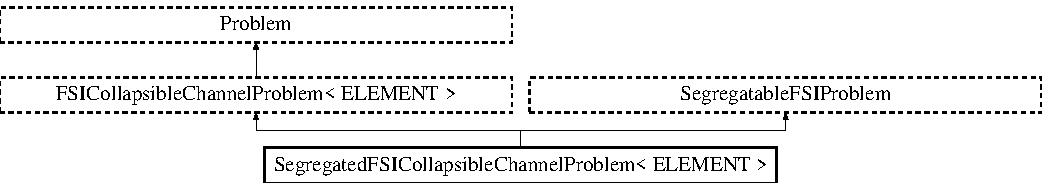
\includegraphics[height=2.463343cm]{classSegregatedFSICollapsibleChannelProblem}
\end{center}
\end{figure}
\subsection*{Public Member Functions}
\begin{DoxyCompactItemize}
\item 
\hyperlink{classSegregatedFSICollapsibleChannelProblem_ac762b472c2baafa23dae6b9ce38f31da}{Segregated\+F\+S\+I\+Collapsible\+Channel\+Problem} (const unsigned \&nup, const unsigned \&ncollapsible, const unsigned \&ndown, const unsigned \&ny, const double \&lup, const double \&lcollapsible, const double \&ldown, const double \&ly, const bool \&displ\+\_\+control, const bool \&steady\+\_\+flag)
\begin{DoxyCompactList}\small\item\em Constructor\+: The arguments are the same as the original (non-\/segregated) problem, namely, numbers of elements and lengths of different sections of the domain. \end{DoxyCompactList}\item 
\hyperlink{classSegregatedFSICollapsibleChannelProblem_aa51bac3f0323fafcc86ff0bf0f6c010c}{$\sim$\+Segregated\+F\+S\+I\+Collapsible\+Channel\+Problem} ()
\begin{DoxyCompactList}\small\item\em Empty Destructor. \end{DoxyCompactList}\item 
void \hyperlink{classSegregatedFSICollapsibleChannelProblem_aa473522c98c5b70b8d35c0a7cdb1e42c}{identify\+\_\+fluid\+\_\+and\+\_\+solid\+\_\+dofs} (Vector$<$ Data $\ast$$>$ \&fluid\+\_\+data\+\_\+pt, Vector$<$ Data $\ast$$>$ \&solid\+\_\+data\+\_\+pt, Mesh $\ast$\&fluid\+\_\+mesh\+\_\+pt, Mesh $\ast$\&solid\+\_\+mesh\+\_\+pt)
\begin{DoxyCompactList}\small\item\em Identify the fluid and solid Data and meshes that contain only elements involved in the respective sub-\/problems. This is a specific implementation of a pure virtual function in the Segregatable\+F\+S\+I\+Problem base class. \end{DoxyCompactList}\item 
void \hyperlink{classSegregatedFSICollapsibleChannelProblem_a2613090b2abf3809de381da12f1cd0d2}{actions\+\_\+before\+\_\+newton\+\_\+convergence\+\_\+check} ()
\begin{DoxyCompactList}\small\item\em Update nodal positions in the fluid mesh in response to changes in the wall displacement field after every Newton step in a monolithic or segregated solid solve. Note the use of the (protected) flag Solve\+\_\+type, which can take the values Full\+\_\+solve, Fluid\+\_\+solve or Solid\+\_\+solve. This flag is used to allow specification of different actions depending on the precise solve taking place. \end{DoxyCompactList}\item 
void \hyperlink{classSegregatedFSICollapsibleChannelProblem_a8ee14a1d4ab159c9b28dfcb177dc7c57}{actions\+\_\+before\+\_\+segregated\+\_\+convergence\+\_\+check} ()
\item 
void \hyperlink{classSegregatedFSICollapsibleChannelProblem_a0f7364ea880f2e740e1960830246e028}{doc\+\_\+solution} (Doc\+Info \&doc\+\_\+info)
\begin{DoxyCompactList}\small\item\em Document the solution. \end{DoxyCompactList}\item 
void \hyperlink{classSegregatedFSICollapsibleChannelProblem_a9a6b0dfeda9eb0d4c50e195768c93e37}{steady\+\_\+run} ()
\begin{DoxyCompactList}\small\item\em Perform a steady run. \end{DoxyCompactList}\end{DoxyCompactItemize}
\subsection*{Additional Inherited Members}


\subsection{Detailed Description}
\subsubsection*{template$<$class E\+L\+E\+M\+E\+NT$>$\newline
class Segregated\+F\+S\+I\+Collapsible\+Channel\+Problem$<$ E\+L\+E\+M\+E\+N\+T $>$}

Problem class -- add segregated solver capability to an existing problem. 

Definition at line 90 of file simple\+\_\+segregated\+\_\+driver.\+cc.



\subsection{Constructor \& Destructor Documentation}
\mbox{\Hypertarget{classSegregatedFSICollapsibleChannelProblem_ac762b472c2baafa23dae6b9ce38f31da}\label{classSegregatedFSICollapsibleChannelProblem_ac762b472c2baafa23dae6b9ce38f31da}} 
\index{Segregated\+F\+S\+I\+Collapsible\+Channel\+Problem@{Segregated\+F\+S\+I\+Collapsible\+Channel\+Problem}!Segregated\+F\+S\+I\+Collapsible\+Channel\+Problem@{Segregated\+F\+S\+I\+Collapsible\+Channel\+Problem}}
\index{Segregated\+F\+S\+I\+Collapsible\+Channel\+Problem@{Segregated\+F\+S\+I\+Collapsible\+Channel\+Problem}!Segregated\+F\+S\+I\+Collapsible\+Channel\+Problem@{Segregated\+F\+S\+I\+Collapsible\+Channel\+Problem}}
\subsubsection{\texorpdfstring{Segregated\+F\+S\+I\+Collapsible\+Channel\+Problem()}{SegregatedFSICollapsibleChannelProblem()}}
{\footnotesize\ttfamily template$<$class E\+L\+E\+M\+E\+NT $>$ \\
\hyperlink{classSegregatedFSICollapsibleChannelProblem}{Segregated\+F\+S\+I\+Collapsible\+Channel\+Problem}$<$ E\+L\+E\+M\+E\+NT $>$\+::\hyperlink{classSegregatedFSICollapsibleChannelProblem}{Segregated\+F\+S\+I\+Collapsible\+Channel\+Problem} (\begin{DoxyParamCaption}\item[{const unsigned \&}]{nup,  }\item[{const unsigned \&}]{ncollapsible,  }\item[{const unsigned \&}]{ndown,  }\item[{const unsigned \&}]{ny,  }\item[{const double \&}]{lup,  }\item[{const double \&}]{lcollapsible,  }\item[{const double \&}]{ldown,  }\item[{const double \&}]{ly,  }\item[{const bool \&}]{displ\+\_\+control,  }\item[{const bool \&}]{steady\+\_\+flag }\end{DoxyParamCaption})}



Constructor\+: The arguments are the same as the original (non-\/segregated) problem, namely, numbers of elements and lengths of different sections of the domain. 

Constructor for the collapsible channel problem. 

Definition at line 172 of file simple\+\_\+segregated\+\_\+driver.\+cc.



References Flags\+::\+Convergence\+\_\+criterion, Flags\+::\+Convergence\+\_\+tolerance, Segregated\+F\+S\+I\+Collapsible\+Channel\+Problem$<$ E\+L\+E\+M\+E\+N\+T $>$\+::identify\+\_\+fluid\+\_\+and\+\_\+solid\+\_\+dofs(), Flags\+::\+Omega\+\_\+under\+\_\+relax, Flags\+::\+Use\+\_\+irons\+\_\+and\+\_\+tuck\+\_\+extrapolation, and Flags\+::\+Use\+\_\+pointwise\+\_\+aitken.



Referenced by Segregated\+F\+S\+I\+Collapsible\+Channel\+Problem$<$ E\+L\+E\+M\+E\+N\+T $>$\+::actions\+\_\+before\+\_\+segregated\+\_\+convergence\+\_\+check().

\mbox{\Hypertarget{classSegregatedFSICollapsibleChannelProblem_aa51bac3f0323fafcc86ff0bf0f6c010c}\label{classSegregatedFSICollapsibleChannelProblem_aa51bac3f0323fafcc86ff0bf0f6c010c}} 
\index{Segregated\+F\+S\+I\+Collapsible\+Channel\+Problem@{Segregated\+F\+S\+I\+Collapsible\+Channel\+Problem}!````~Segregated\+F\+S\+I\+Collapsible\+Channel\+Problem@{$\sim$\+Segregated\+F\+S\+I\+Collapsible\+Channel\+Problem}}
\index{````~Segregated\+F\+S\+I\+Collapsible\+Channel\+Problem@{$\sim$\+Segregated\+F\+S\+I\+Collapsible\+Channel\+Problem}!Segregated\+F\+S\+I\+Collapsible\+Channel\+Problem@{Segregated\+F\+S\+I\+Collapsible\+Channel\+Problem}}
\subsubsection{\texorpdfstring{$\sim$\+Segregated\+F\+S\+I\+Collapsible\+Channel\+Problem()}{~SegregatedFSICollapsibleChannelProblem()}}
{\footnotesize\ttfamily template$<$class E\+L\+E\+M\+E\+NT $>$ \\
\hyperlink{classSegregatedFSICollapsibleChannelProblem}{Segregated\+F\+S\+I\+Collapsible\+Channel\+Problem}$<$ E\+L\+E\+M\+E\+NT $>$\+::$\sim$\hyperlink{classSegregatedFSICollapsibleChannelProblem}{Segregated\+F\+S\+I\+Collapsible\+Channel\+Problem} (\begin{DoxyParamCaption}{ }\end{DoxyParamCaption})\hspace{0.3cm}{\ttfamily [inline]}}



Empty Destructor. 



Definition at line 112 of file simple\+\_\+segregated\+\_\+driver.\+cc.



\subsection{Member Function Documentation}
\mbox{\Hypertarget{classSegregatedFSICollapsibleChannelProblem_a2613090b2abf3809de381da12f1cd0d2}\label{classSegregatedFSICollapsibleChannelProblem_a2613090b2abf3809de381da12f1cd0d2}} 
\index{Segregated\+F\+S\+I\+Collapsible\+Channel\+Problem@{Segregated\+F\+S\+I\+Collapsible\+Channel\+Problem}!actions\+\_\+before\+\_\+newton\+\_\+convergence\+\_\+check@{actions\+\_\+before\+\_\+newton\+\_\+convergence\+\_\+check}}
\index{actions\+\_\+before\+\_\+newton\+\_\+convergence\+\_\+check@{actions\+\_\+before\+\_\+newton\+\_\+convergence\+\_\+check}!Segregated\+F\+S\+I\+Collapsible\+Channel\+Problem@{Segregated\+F\+S\+I\+Collapsible\+Channel\+Problem}}
\subsubsection{\texorpdfstring{actions\+\_\+before\+\_\+newton\+\_\+convergence\+\_\+check()}{actions\_before\_newton\_convergence\_check()}}
{\footnotesize\ttfamily template$<$class E\+L\+E\+M\+E\+NT $>$ \\
void \hyperlink{classSegregatedFSICollapsibleChannelProblem}{Segregated\+F\+S\+I\+Collapsible\+Channel\+Problem}$<$ E\+L\+E\+M\+E\+NT $>$\+::actions\+\_\+before\+\_\+newton\+\_\+convergence\+\_\+check (\begin{DoxyParamCaption}{ }\end{DoxyParamCaption})\hspace{0.3cm}{\ttfamily [inline]}}



Update nodal positions in the fluid mesh in response to changes in the wall displacement field after every Newton step in a monolithic or segregated solid solve. Note the use of the (protected) flag Solve\+\_\+type, which can take the values Full\+\_\+solve, Fluid\+\_\+solve or Solid\+\_\+solve. This flag is used to allow specification of different actions depending on the precise solve taking place. 



Definition at line 133 of file simple\+\_\+segregated\+\_\+driver.\+cc.

\mbox{\Hypertarget{classSegregatedFSICollapsibleChannelProblem_a8ee14a1d4ab159c9b28dfcb177dc7c57}\label{classSegregatedFSICollapsibleChannelProblem_a8ee14a1d4ab159c9b28dfcb177dc7c57}} 
\index{Segregated\+F\+S\+I\+Collapsible\+Channel\+Problem@{Segregated\+F\+S\+I\+Collapsible\+Channel\+Problem}!actions\+\_\+before\+\_\+segregated\+\_\+convergence\+\_\+check@{actions\+\_\+before\+\_\+segregated\+\_\+convergence\+\_\+check}}
\index{actions\+\_\+before\+\_\+segregated\+\_\+convergence\+\_\+check@{actions\+\_\+before\+\_\+segregated\+\_\+convergence\+\_\+check}!Segregated\+F\+S\+I\+Collapsible\+Channel\+Problem@{Segregated\+F\+S\+I\+Collapsible\+Channel\+Problem}}
\subsubsection{\texorpdfstring{actions\+\_\+before\+\_\+segregated\+\_\+convergence\+\_\+check()}{actions\_before\_segregated\_convergence\_check()}}
{\footnotesize\ttfamily template$<$class E\+L\+E\+M\+E\+NT $>$ \\
void \hyperlink{classSegregatedFSICollapsibleChannelProblem}{Segregated\+F\+S\+I\+Collapsible\+Channel\+Problem}$<$ E\+L\+E\+M\+E\+NT $>$\+::actions\+\_\+before\+\_\+segregated\+\_\+convergence\+\_\+check (\begin{DoxyParamCaption}{ }\end{DoxyParamCaption})\hspace{0.3cm}{\ttfamily [inline]}}

Update nodal positions in the fluid mesh in response to any changes in the wall displacement field after every segregated solve. This is not strictly necessary because we do the solid solve last, which performs its own node update before the convergence check of the sub problem. It remains here because if we were solving in a completely segregated fashion a node update would be required for the fluid mesh in the final converged solution to be consistent with the solid positions. 

Definition at line 151 of file simple\+\_\+segregated\+\_\+driver.\+cc.



References Segregated\+F\+S\+I\+Collapsible\+Channel\+Problem$<$ E\+L\+E\+M\+E\+N\+T $>$\+::\+Segregated\+F\+S\+I\+Collapsible\+Channel\+Problem().

\mbox{\Hypertarget{classSegregatedFSICollapsibleChannelProblem_a0f7364ea880f2e740e1960830246e028}\label{classSegregatedFSICollapsibleChannelProblem_a0f7364ea880f2e740e1960830246e028}} 
\index{Segregated\+F\+S\+I\+Collapsible\+Channel\+Problem@{Segregated\+F\+S\+I\+Collapsible\+Channel\+Problem}!doc\+\_\+solution@{doc\+\_\+solution}}
\index{doc\+\_\+solution@{doc\+\_\+solution}!Segregated\+F\+S\+I\+Collapsible\+Channel\+Problem@{Segregated\+F\+S\+I\+Collapsible\+Channel\+Problem}}
\subsubsection{\texorpdfstring{doc\+\_\+solution()}{doc\_solution()}}
{\footnotesize\ttfamily template$<$class E\+L\+E\+M\+E\+NT $>$ \\
void \hyperlink{classSegregatedFSICollapsibleChannelProblem}{Segregated\+F\+S\+I\+Collapsible\+Channel\+Problem}$<$ E\+L\+E\+M\+E\+NT $>$\+::doc\+\_\+solution (\begin{DoxyParamCaption}\item[{Doc\+Info \&}]{doc\+\_\+info }\end{DoxyParamCaption})}



Document the solution. 



Definition at line 330 of file simple\+\_\+segregated\+\_\+driver.\+cc.



References F\+S\+I\+Collapsible\+Channel\+Problem$<$ E\+L\+E\+M\+E\+N\+T $>$\+::bulk\+\_\+mesh\+\_\+pt(), and F\+S\+I\+Collapsible\+Channel\+Problem$<$ E\+L\+E\+M\+E\+N\+T $>$\+::wall\+\_\+mesh\+\_\+pt().



Referenced by Segregated\+F\+S\+I\+Collapsible\+Channel\+Problem$<$ E\+L\+E\+M\+E\+N\+T $>$\+::steady\+\_\+run().

\mbox{\Hypertarget{classSegregatedFSICollapsibleChannelProblem_aa473522c98c5b70b8d35c0a7cdb1e42c}\label{classSegregatedFSICollapsibleChannelProblem_aa473522c98c5b70b8d35c0a7cdb1e42c}} 
\index{Segregated\+F\+S\+I\+Collapsible\+Channel\+Problem@{Segregated\+F\+S\+I\+Collapsible\+Channel\+Problem}!identify\+\_\+fluid\+\_\+and\+\_\+solid\+\_\+dofs@{identify\+\_\+fluid\+\_\+and\+\_\+solid\+\_\+dofs}}
\index{identify\+\_\+fluid\+\_\+and\+\_\+solid\+\_\+dofs@{identify\+\_\+fluid\+\_\+and\+\_\+solid\+\_\+dofs}!Segregated\+F\+S\+I\+Collapsible\+Channel\+Problem@{Segregated\+F\+S\+I\+Collapsible\+Channel\+Problem}}
\subsubsection{\texorpdfstring{identify\+\_\+fluid\+\_\+and\+\_\+solid\+\_\+dofs()}{identify\_fluid\_and\_solid\_dofs()}}
{\footnotesize\ttfamily template$<$class E\+L\+E\+M\+E\+NT $>$ \\
void \hyperlink{classSegregatedFSICollapsibleChannelProblem}{Segregated\+F\+S\+I\+Collapsible\+Channel\+Problem}$<$ E\+L\+E\+M\+E\+NT $>$\+::identify\+\_\+fluid\+\_\+and\+\_\+solid\+\_\+dofs (\begin{DoxyParamCaption}\item[{Vector$<$ Data $\ast$$>$ \&}]{fluid\+\_\+data\+\_\+pt,  }\item[{Vector$<$ Data $\ast$$>$ \&}]{solid\+\_\+data\+\_\+pt,  }\item[{Mesh $\ast$\&}]{fluid\+\_\+mesh\+\_\+pt,  }\item[{Mesh $\ast$\&}]{solid\+\_\+mesh\+\_\+pt }\end{DoxyParamCaption})}



Identify the fluid and solid Data and meshes that contain only elements involved in the respective sub-\/problems. This is a specific implementation of a pure virtual function in the Segregatable\+F\+S\+I\+Problem base class. 

Identify the fluid and solid Data and the meshes that contain only elements that are involved in the respective sub-\/problems. This implements a pure virtual function in the Segregatable\+F\+S\+I\+Problem base class. 

Definition at line 248 of file simple\+\_\+segregated\+\_\+driver.\+cc.



References F\+S\+I\+Collapsible\+Channel\+Problem$<$ E\+L\+E\+M\+E\+N\+T $>$\+::bulk\+\_\+mesh\+\_\+pt(), F\+S\+I\+Collapsible\+Channel\+Problem$<$ E\+L\+E\+M\+E\+N\+T $>$\+::\+Displ\+\_\+control, F\+S\+I\+Collapsible\+Channel\+Problem$<$ E\+L\+E\+M\+E\+N\+T $>$\+::\+Displ\+\_\+control\+\_\+mesh\+\_\+pt, Global\+\_\+\+Physical\+\_\+\+Variables\+::\+P\+\_\+ext\+\_\+data\+\_\+pt, and F\+S\+I\+Collapsible\+Channel\+Problem$<$ E\+L\+E\+M\+E\+N\+T $>$\+::wall\+\_\+mesh\+\_\+pt().



Referenced by Segregated\+F\+S\+I\+Collapsible\+Channel\+Problem$<$ E\+L\+E\+M\+E\+N\+T $>$\+::\+Segregated\+F\+S\+I\+Collapsible\+Channel\+Problem().

\mbox{\Hypertarget{classSegregatedFSICollapsibleChannelProblem_a9a6b0dfeda9eb0d4c50e195768c93e37}\label{classSegregatedFSICollapsibleChannelProblem_a9a6b0dfeda9eb0d4c50e195768c93e37}} 
\index{Segregated\+F\+S\+I\+Collapsible\+Channel\+Problem@{Segregated\+F\+S\+I\+Collapsible\+Channel\+Problem}!steady\+\_\+run@{steady\+\_\+run}}
\index{steady\+\_\+run@{steady\+\_\+run}!Segregated\+F\+S\+I\+Collapsible\+Channel\+Problem@{Segregated\+F\+S\+I\+Collapsible\+Channel\+Problem}}
\subsubsection{\texorpdfstring{steady\+\_\+run()}{steady\_run()}}
{\footnotesize\ttfamily template$<$class E\+L\+E\+M\+E\+NT $>$ \\
void \hyperlink{classSegregatedFSICollapsibleChannelProblem}{Segregated\+F\+S\+I\+Collapsible\+Channel\+Problem}$<$ E\+L\+E\+M\+E\+NT $>$\+::steady\+\_\+run (\begin{DoxyParamCaption}{ }\end{DoxyParamCaption})\hspace{0.3cm}{\ttfamily [virtual]}}



Perform a steady run. 

Perform a steady run in which the external pressure (or presribed displacement) is varied causing the channel to collapse. 

Reimplemented from \hyperlink{classFSICollapsibleChannelProblem_a299ba7d5819e7871eae7e331d1abab8b}{F\+S\+I\+Collapsible\+Channel\+Problem$<$ E\+L\+E\+M\+E\+N\+T $>$}.



Definition at line 363 of file simple\+\_\+segregated\+\_\+driver.\+cc.



References F\+S\+I\+Collapsible\+Channel\+Problem$<$ E\+L\+E\+M\+E\+N\+T $>$\+::\+Displ\+\_\+control, Segregated\+F\+S\+I\+Collapsible\+Channel\+Problem$<$ E\+L\+E\+M\+E\+N\+T $>$\+::doc\+\_\+solution(), Flags\+::\+Nsteps, Global\+\_\+\+Physical\+\_\+\+Variables\+::\+P\+\_\+ext\+\_\+data\+\_\+pt, Global\+\_\+\+Physical\+\_\+\+Variables\+::\+Pmax, Global\+\_\+\+Physical\+\_\+\+Variables\+::\+Pmin, F\+S\+I\+Collapsible\+Channel\+Problem$<$ E\+L\+E\+M\+E\+N\+T $>$\+::set\+\_\+initial\+\_\+condition(), Flags\+::\+Use\+\_\+segregated\+\_\+solver, and Global\+\_\+\+Physical\+\_\+\+Variables\+::\+Yprescr.



The documentation for this class was generated from the following file\+:\begin{DoxyCompactItemize}
\item 
\hyperlink{simple__segregated__driver_8cc}{simple\+\_\+segregated\+\_\+driver.\+cc}\end{DoxyCompactItemize}

\hypertarget{classUndeformedWall}{}\section{Undeformed\+Wall Class Reference}
\label{classUndeformedWall}\index{Undeformed\+Wall@{Undeformed\+Wall}}
Inheritance diagram for Undeformed\+Wall\+:\begin{figure}[H]
\begin{center}
\leavevmode
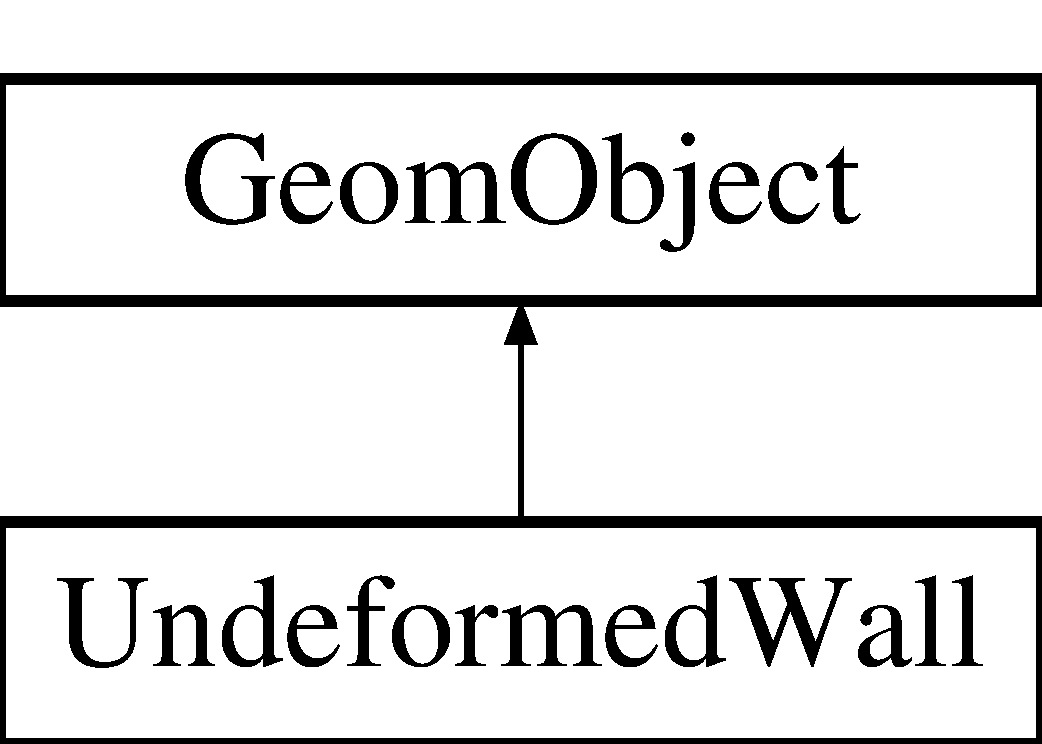
\includegraphics[height=2.000000cm]{classUndeformedWall}
\end{center}
\end{figure}
\subsection*{Public Member Functions}
\begin{DoxyCompactItemize}
\item 
\hyperlink{classUndeformedWall_ad09cfdcd234be0ab47eb97a8a470602a}{Undeformed\+Wall} (const double \&x0, const double \&h)
\begin{DoxyCompactList}\small\item\em Constructor\+: arguments are the starting point and the height above y=0. \end{DoxyCompactList}\item 
void \hyperlink{classUndeformedWall_ab0410681e2096091319a79e79937cba3}{position} (const Vector$<$ double $>$ \&zeta, Vector$<$ double $>$ \&r) const
\begin{DoxyCompactList}\small\item\em Position vector at Lagrangian coordinate zeta. \end{DoxyCompactList}\item 
void \hyperlink{classUndeformedWall_a9cbb52e30fd47d1841c1c3dc812f4b96}{position} (const unsigned \&t, const Vector$<$ double $>$ \&zeta, Vector$<$ double $>$ \&r) const
\begin{DoxyCompactList}\small\item\em Parametrised position on object\+: r(zeta). Evaluated at previous timestep. t=0\+: current time; t$>$0\+: previous timestep. Calls steady version. \end{DoxyCompactList}\item 
void \hyperlink{classUndeformedWall_a6e25add1790f0de89bbe6840dae66a93}{d2position} (const Vector$<$ double $>$ \&zeta, Vector$<$ double $>$ \&r, Dense\+Matrix$<$ double $>$ \&drdzeta, Rank\+Three\+Tensor$<$ double $>$ \&ddrdzeta) const
\begin{DoxyCompactList}\small\item\em Posn vector and its 1st \& 2nd derivatives w.\+r.\+t. to coordinates\+: $ \frac{dR_i}{d \zeta_\alpha}$ = drdzeta(alpha,i). $ \frac{d^2R_i}{d \zeta_\alpha d \zeta_\beta}$ = ddrdzeta(alpha,beta,i). Evaluated at current time. \end{DoxyCompactList}\item 
\hyperlink{classUndeformedWall_ad09cfdcd234be0ab47eb97a8a470602a}{Undeformed\+Wall} (const double \&x0, const double \&h)
\begin{DoxyCompactList}\small\item\em Constructor\+: arguments are the starting point and the height above y=0. \end{DoxyCompactList}\item 
void \hyperlink{classUndeformedWall_ab0410681e2096091319a79e79937cba3}{position} (const Vector$<$ double $>$ \&zeta, Vector$<$ double $>$ \&r) const
\begin{DoxyCompactList}\small\item\em Position vector at Lagrangian coordinate zeta. \end{DoxyCompactList}\item 
void \hyperlink{classUndeformedWall_a9cbb52e30fd47d1841c1c3dc812f4b96}{position} (const unsigned \&t, const Vector$<$ double $>$ \&zeta, Vector$<$ double $>$ \&r) const
\begin{DoxyCompactList}\small\item\em Parametrised position on object\+: r(zeta). Evaluated at previous timestep. t=0\+: current time; t$>$0\+: previous timestep. Calls steady version. \end{DoxyCompactList}\item 
virtual void \hyperlink{classUndeformedWall_a709e65fc95e9443a886125e455595e5d}{d2position} (const Vector$<$ double $>$ \&zeta, Vector$<$ double $>$ \&r, Dense\+Matrix$<$ double $>$ \&drdzeta, Rank\+Three\+Tensor$<$ double $>$ \&ddrdzeta) const
\begin{DoxyCompactList}\small\item\em Posn vector and its 1st \& 2nd derivatives w.\+r.\+t. to coordinates\+: $ \frac{dR_i}{d \zeta_\alpha}$ = drdzeta(alpha,i). $ \frac{d^2R_i}{d \zeta_\alpha d \zeta_\beta}$ = ddrdzeta(alpha,beta,i). Evaluated at current time. \end{DoxyCompactList}\item 
\hyperlink{classUndeformedWall_ad09cfdcd234be0ab47eb97a8a470602a}{Undeformed\+Wall} (const double \&x0, const double \&h)
\begin{DoxyCompactList}\small\item\em Constructor\+: arguments are the starting point and the height above y=0. \end{DoxyCompactList}\item 
void \hyperlink{classUndeformedWall_ab0410681e2096091319a79e79937cba3}{position} (const Vector$<$ double $>$ \&zeta, Vector$<$ double $>$ \&r) const
\begin{DoxyCompactList}\small\item\em Position vector at Lagrangian coordinate zeta. \end{DoxyCompactList}\item 
void \hyperlink{classUndeformedWall_a9cbb52e30fd47d1841c1c3dc812f4b96}{position} (const unsigned \&t, const Vector$<$ double $>$ \&zeta, Vector$<$ double $>$ \&r) const
\begin{DoxyCompactList}\small\item\em Parametrised position on object\+: r(zeta). Evaluated at previous timestep. t=0\+: current time; t$>$0\+: previous timestep. Calls steady version. \end{DoxyCompactList}\item 
virtual void \hyperlink{classUndeformedWall_a709e65fc95e9443a886125e455595e5d}{d2position} (const Vector$<$ double $>$ \&zeta, Vector$<$ double $>$ \&r, Dense\+Matrix$<$ double $>$ \&drdzeta, Rank\+Three\+Tensor$<$ double $>$ \&ddrdzeta) const
\begin{DoxyCompactList}\small\item\em Posn vector and its 1st \& 2nd derivatives w.\+r.\+t. to coordinates\+: $ \frac{dR_i}{d \zeta_\alpha}$ = drdzeta(alpha,i). $ \frac{d^2R_i}{d \zeta_\alpha d \zeta_\beta}$ = ddrdzeta(alpha,beta,i). Evaluated at current time. \end{DoxyCompactList}\item 
\hyperlink{classUndeformedWall_ad09cfdcd234be0ab47eb97a8a470602a}{Undeformed\+Wall} (const double \&x0, const double \&h)
\begin{DoxyCompactList}\small\item\em Constructor\+: arguments are the starting point and the height above y=0. \end{DoxyCompactList}\item 
void \hyperlink{classUndeformedWall_ab0410681e2096091319a79e79937cba3}{position} (const Vector$<$ double $>$ \&zeta, Vector$<$ double $>$ \&r) const
\begin{DoxyCompactList}\small\item\em Position vector at Lagrangian coordinate zeta. \end{DoxyCompactList}\item 
void \hyperlink{classUndeformedWall_a9cbb52e30fd47d1841c1c3dc812f4b96}{position} (const unsigned \&t, const Vector$<$ double $>$ \&zeta, Vector$<$ double $>$ \&r) const
\begin{DoxyCompactList}\small\item\em Parametrised position on object\+: r(zeta). Evaluated at previous timestep. t=0\+: current time; t$>$0\+: previous timestep. Calls steady version. \end{DoxyCompactList}\item 
virtual void \hyperlink{classUndeformedWall_a709e65fc95e9443a886125e455595e5d}{d2position} (const Vector$<$ double $>$ \&zeta, Vector$<$ double $>$ \&r, Dense\+Matrix$<$ double $>$ \&drdzeta, Rank\+Three\+Tensor$<$ double $>$ \&ddrdzeta) const
\begin{DoxyCompactList}\small\item\em Posn vector and its 1st \& 2nd derivatives w.\+r.\+t. to coordinates\+: $ \frac{dR_i}{d \zeta_\alpha}$ = drdzeta(alpha,i). $ \frac{d^2R_i}{d \zeta_\alpha d \zeta_\beta}$ = ddrdzeta(alpha,beta,i). Evaluated at current time. \end{DoxyCompactList}\end{DoxyCompactItemize}
\subsection*{Private Attributes}
\begin{DoxyCompactItemize}
\item 
double \hyperlink{classUndeformedWall_a7ab875c46fef905df33eb47e0336581b}{X0}
\begin{DoxyCompactList}\small\item\em x position of the undeformed beam\textquotesingle{}s left end. \end{DoxyCompactList}\item 
double \hyperlink{classUndeformedWall_a4525dbe0b5d2108ee51f16bee9af88ef}{H}
\begin{DoxyCompactList}\small\item\em Height of the undeformed wall above y=0. \end{DoxyCompactList}\end{DoxyCompactItemize}


\subsection{Detailed Description}
Undeformed wall is a steady, straight 1D line in 2D space \[ x = X_0 + \zeta \] \[ y = H \] 

Definition at line 100 of file fsi\+\_\+collapsible\+\_\+channel.\+cc.



\subsection{Constructor \& Destructor Documentation}
\mbox{\Hypertarget{classUndeformedWall_ad09cfdcd234be0ab47eb97a8a470602a}\label{classUndeformedWall_ad09cfdcd234be0ab47eb97a8a470602a}} 
\index{Undeformed\+Wall@{Undeformed\+Wall}!Undeformed\+Wall@{Undeformed\+Wall}}
\index{Undeformed\+Wall@{Undeformed\+Wall}!Undeformed\+Wall@{Undeformed\+Wall}}
\subsubsection{\texorpdfstring{Undeformed\+Wall()}{UndeformedWall()}\hspace{0.1cm}{\footnotesize\ttfamily [1/4]}}
{\footnotesize\ttfamily Undeformed\+Wall\+::\+Undeformed\+Wall (\begin{DoxyParamCaption}\item[{const double \&}]{x0,  }\item[{const double \&}]{h }\end{DoxyParamCaption})\hspace{0.3cm}{\ttfamily [inline]}}



Constructor\+: arguments are the starting point and the height above y=0. 



Definition at line 107 of file fsi\+\_\+collapsible\+\_\+channel.\+cc.



References Global\+\_\+\+Physical\+\_\+\+Variables\+::H.

\mbox{\Hypertarget{classUndeformedWall_ad09cfdcd234be0ab47eb97a8a470602a}\label{classUndeformedWall_ad09cfdcd234be0ab47eb97a8a470602a}} 
\index{Undeformed\+Wall@{Undeformed\+Wall}!Undeformed\+Wall@{Undeformed\+Wall}}
\index{Undeformed\+Wall@{Undeformed\+Wall}!Undeformed\+Wall@{Undeformed\+Wall}}
\subsubsection{\texorpdfstring{Undeformed\+Wall()}{UndeformedWall()}\hspace{0.1cm}{\footnotesize\ttfamily [2/4]}}
{\footnotesize\ttfamily Undeformed\+Wall\+::\+Undeformed\+Wall (\begin{DoxyParamCaption}\item[{const double \&}]{x0,  }\item[{const double \&}]{h }\end{DoxyParamCaption})\hspace{0.3cm}{\ttfamily [inline]}}



Constructor\+: arguments are the starting point and the height above y=0. 



Definition at line 106 of file fsi\+\_\+collapsible\+\_\+channel\+\_\+adapt.\+cc.



References Global\+\_\+\+Physical\+\_\+\+Variables\+::H.

\mbox{\Hypertarget{classUndeformedWall_ad09cfdcd234be0ab47eb97a8a470602a}\label{classUndeformedWall_ad09cfdcd234be0ab47eb97a8a470602a}} 
\index{Undeformed\+Wall@{Undeformed\+Wall}!Undeformed\+Wall@{Undeformed\+Wall}}
\index{Undeformed\+Wall@{Undeformed\+Wall}!Undeformed\+Wall@{Undeformed\+Wall}}
\subsubsection{\texorpdfstring{Undeformed\+Wall()}{UndeformedWall()}\hspace{0.1cm}{\footnotesize\ttfamily [3/4]}}
{\footnotesize\ttfamily Undeformed\+Wall\+::\+Undeformed\+Wall (\begin{DoxyParamCaption}\item[{const double \&}]{x0,  }\item[{const double \&}]{h }\end{DoxyParamCaption})\hspace{0.3cm}{\ttfamily [inline]}}



Constructor\+: arguments are the starting point and the height above y=0. 



Definition at line 146 of file fsi\+\_\+pseudo\+\_\+solid\+\_\+collapsible\+\_\+channel.\+cc.



References Global\+\_\+\+Physical\+\_\+\+Variables\+::H.

\mbox{\Hypertarget{classUndeformedWall_ad09cfdcd234be0ab47eb97a8a470602a}\label{classUndeformedWall_ad09cfdcd234be0ab47eb97a8a470602a}} 
\index{Undeformed\+Wall@{Undeformed\+Wall}!Undeformed\+Wall@{Undeformed\+Wall}}
\index{Undeformed\+Wall@{Undeformed\+Wall}!Undeformed\+Wall@{Undeformed\+Wall}}
\subsubsection{\texorpdfstring{Undeformed\+Wall()}{UndeformedWall()}\hspace{0.1cm}{\footnotesize\ttfamily [4/4]}}
{\footnotesize\ttfamily Undeformed\+Wall\+::\+Undeformed\+Wall (\begin{DoxyParamCaption}\item[{const double \&}]{x0,  }\item[{const double \&}]{h }\end{DoxyParamCaption})\hspace{0.3cm}{\ttfamily [inline]}}



Constructor\+: arguments are the starting point and the height above y=0. 



Definition at line 151 of file fsi\+\_\+pseudo\+\_\+solid\+\_\+collapsible\+\_\+channel\+\_\+adapt.\+cc.



References Global\+\_\+\+Physical\+\_\+\+Variables\+::H.



\subsection{Member Function Documentation}
\mbox{\Hypertarget{classUndeformedWall_a709e65fc95e9443a886125e455595e5d}\label{classUndeformedWall_a709e65fc95e9443a886125e455595e5d}} 
\index{Undeformed\+Wall@{Undeformed\+Wall}!d2position@{d2position}}
\index{d2position@{d2position}!Undeformed\+Wall@{Undeformed\+Wall}}
\subsubsection{\texorpdfstring{d2position()}{d2position()}\hspace{0.1cm}{\footnotesize\ttfamily [1/4]}}
{\footnotesize\ttfamily virtual void Undeformed\+Wall\+::d2position (\begin{DoxyParamCaption}\item[{const Vector$<$ double $>$ \&}]{zeta,  }\item[{Vector$<$ double $>$ \&}]{r,  }\item[{Dense\+Matrix$<$ double $>$ \&}]{drdzeta,  }\item[{Rank\+Three\+Tensor$<$ double $>$ \&}]{ddrdzeta }\end{DoxyParamCaption}) const\hspace{0.3cm}{\ttfamily [inline]}, {\ttfamily [virtual]}}



Posn vector and its 1st \& 2nd derivatives w.\+r.\+t. to coordinates\+: $ \frac{dR_i}{d \zeta_\alpha}$ = drdzeta(alpha,i). $ \frac{d^2R_i}{d \zeta_\alpha d \zeta_\beta}$ = ddrdzeta(alpha,beta,i). Evaluated at current time. 



Definition at line 139 of file fsi\+\_\+collapsible\+\_\+channel\+\_\+adapt.\+cc.



References Global\+\_\+\+Physical\+\_\+\+Variables\+::H, Global\+\_\+\+Physical\+\_\+\+Variables\+::load(), Global\+\_\+\+Physical\+\_\+\+Variables\+::\+P\+\_\+ext, Global\+\_\+\+Physical\+\_\+\+Variables\+::\+P\+\_\+up, Global\+\_\+\+Physical\+\_\+\+Variables\+::prescribed\+\_\+traction(), Global\+\_\+\+Physical\+\_\+\+Variables\+::Q, Global\+\_\+\+Physical\+\_\+\+Variables\+::\+Re, Global\+\_\+\+Physical\+\_\+\+Variables\+::\+Re\+St, and Global\+\_\+\+Physical\+\_\+\+Variables\+::\+Sigma0.

\mbox{\Hypertarget{classUndeformedWall_a6e25add1790f0de89bbe6840dae66a93}\label{classUndeformedWall_a6e25add1790f0de89bbe6840dae66a93}} 
\index{Undeformed\+Wall@{Undeformed\+Wall}!d2position@{d2position}}
\index{d2position@{d2position}!Undeformed\+Wall@{Undeformed\+Wall}}
\subsubsection{\texorpdfstring{d2position()}{d2position()}\hspace{0.1cm}{\footnotesize\ttfamily [2/4]}}
{\footnotesize\ttfamily void Undeformed\+Wall\+::d2position (\begin{DoxyParamCaption}\item[{const Vector$<$ double $>$ \&}]{zeta,  }\item[{Vector$<$ double $>$ \&}]{r,  }\item[{Dense\+Matrix$<$ double $>$ \&}]{drdzeta,  }\item[{Rank\+Three\+Tensor$<$ double $>$ \&}]{ddrdzeta }\end{DoxyParamCaption}) const\hspace{0.3cm}{\ttfamily [inline]}}



Posn vector and its 1st \& 2nd derivatives w.\+r.\+t. to coordinates\+: $ \frac{dR_i}{d \zeta_\alpha}$ = drdzeta(alpha,i). $ \frac{d^2R_i}{d \zeta_\alpha d \zeta_\beta}$ = ddrdzeta(alpha,beta,i). Evaluated at current time. 



Definition at line 140 of file fsi\+\_\+collapsible\+\_\+channel.\+cc.



References Global\+\_\+\+Physical\+\_\+\+Variables\+::H.

\mbox{\Hypertarget{classUndeformedWall_a709e65fc95e9443a886125e455595e5d}\label{classUndeformedWall_a709e65fc95e9443a886125e455595e5d}} 
\index{Undeformed\+Wall@{Undeformed\+Wall}!d2position@{d2position}}
\index{d2position@{d2position}!Undeformed\+Wall@{Undeformed\+Wall}}
\subsubsection{\texorpdfstring{d2position()}{d2position()}\hspace{0.1cm}{\footnotesize\ttfamily [3/4]}}
{\footnotesize\ttfamily virtual void Undeformed\+Wall\+::d2position (\begin{DoxyParamCaption}\item[{const Vector$<$ double $>$ \&}]{zeta,  }\item[{Vector$<$ double $>$ \&}]{r,  }\item[{Dense\+Matrix$<$ double $>$ \&}]{drdzeta,  }\item[{Rank\+Three\+Tensor$<$ double $>$ \&}]{ddrdzeta }\end{DoxyParamCaption}) const\hspace{0.3cm}{\ttfamily [inline]}, {\ttfamily [virtual]}}



Posn vector and its 1st \& 2nd derivatives w.\+r.\+t. to coordinates\+: $ \frac{dR_i}{d \zeta_\alpha}$ = drdzeta(alpha,i). $ \frac{d^2R_i}{d \zeta_\alpha d \zeta_\beta}$ = ddrdzeta(alpha,beta,i). Evaluated at current time. 



Definition at line 179 of file fsi\+\_\+pseudo\+\_\+solid\+\_\+collapsible\+\_\+channel.\+cc.



References Global\+\_\+\+Physical\+\_\+\+Variables\+::H, Global\+\_\+\+Physical\+\_\+\+Variables\+::\+P\+\_\+up, Global\+\_\+\+Physical\+\_\+\+Variables\+::\+Re, and Global\+\_\+\+Physical\+\_\+\+Variables\+::\+Re\+St.

\mbox{\Hypertarget{classUndeformedWall_a709e65fc95e9443a886125e455595e5d}\label{classUndeformedWall_a709e65fc95e9443a886125e455595e5d}} 
\index{Undeformed\+Wall@{Undeformed\+Wall}!d2position@{d2position}}
\index{d2position@{d2position}!Undeformed\+Wall@{Undeformed\+Wall}}
\subsubsection{\texorpdfstring{d2position()}{d2position()}\hspace{0.1cm}{\footnotesize\ttfamily [4/4]}}
{\footnotesize\ttfamily virtual void Undeformed\+Wall\+::d2position (\begin{DoxyParamCaption}\item[{const Vector$<$ double $>$ \&}]{zeta,  }\item[{Vector$<$ double $>$ \&}]{r,  }\item[{Dense\+Matrix$<$ double $>$ \&}]{drdzeta,  }\item[{Rank\+Three\+Tensor$<$ double $>$ \&}]{ddrdzeta }\end{DoxyParamCaption}) const\hspace{0.3cm}{\ttfamily [inline]}, {\ttfamily [virtual]}}



Posn vector and its 1st \& 2nd derivatives w.\+r.\+t. to coordinates\+: $ \frac{dR_i}{d \zeta_\alpha}$ = drdzeta(alpha,i). $ \frac{d^2R_i}{d \zeta_\alpha d \zeta_\beta}$ = ddrdzeta(alpha,beta,i). Evaluated at current time. 



Definition at line 184 of file fsi\+\_\+pseudo\+\_\+solid\+\_\+collapsible\+\_\+channel\+\_\+adapt.\+cc.



References Global\+\_\+\+Physical\+\_\+\+Variables\+::H, Global\+\_\+\+Physical\+\_\+\+Variables\+::\+Lambda\+\_\+sq, Global\+\_\+\+Physical\+\_\+\+Variables\+::load(), Global\+\_\+\+Physical\+\_\+\+Variables\+::\+Nu, Global\+\_\+\+Physical\+\_\+\+Variables\+::\+P\+\_\+ext, Global\+\_\+\+Physical\+\_\+\+Variables\+::\+P\+\_\+up, Global\+\_\+\+Physical\+\_\+\+Variables\+::prescribed\+\_\+traction(), Global\+\_\+\+Physical\+\_\+\+Variables\+::Q, Global\+\_\+\+Physical\+\_\+\+Variables\+::\+Re, Global\+\_\+\+Physical\+\_\+\+Variables\+::\+Re\+St, and Global\+\_\+\+Physical\+\_\+\+Variables\+::\+Sigma0.

\mbox{\Hypertarget{classUndeformedWall_ab0410681e2096091319a79e79937cba3}\label{classUndeformedWall_ab0410681e2096091319a79e79937cba3}} 
\index{Undeformed\+Wall@{Undeformed\+Wall}!position@{position}}
\index{position@{position}!Undeformed\+Wall@{Undeformed\+Wall}}
\subsubsection{\texorpdfstring{position()}{position()}\hspace{0.1cm}{\footnotesize\ttfamily [1/8]}}
{\footnotesize\ttfamily void Undeformed\+Wall\+::position (\begin{DoxyParamCaption}\item[{const Vector$<$ double $>$ \&}]{zeta,  }\item[{Vector$<$ double $>$ \&}]{r }\end{DoxyParamCaption}) const\hspace{0.3cm}{\ttfamily [inline]}}



Position vector at Lagrangian coordinate zeta. 



Definition at line 114 of file fsi\+\_\+collapsible\+\_\+channel\+\_\+adapt.\+cc.



References Global\+\_\+\+Physical\+\_\+\+Variables\+::H.

\mbox{\Hypertarget{classUndeformedWall_ab0410681e2096091319a79e79937cba3}\label{classUndeformedWall_ab0410681e2096091319a79e79937cba3}} 
\index{Undeformed\+Wall@{Undeformed\+Wall}!position@{position}}
\index{position@{position}!Undeformed\+Wall@{Undeformed\+Wall}}
\subsubsection{\texorpdfstring{position()}{position()}\hspace{0.1cm}{\footnotesize\ttfamily [2/8]}}
{\footnotesize\ttfamily void Undeformed\+Wall\+::position (\begin{DoxyParamCaption}\item[{const Vector$<$ double $>$ \&}]{zeta,  }\item[{Vector$<$ double $>$ \&}]{r }\end{DoxyParamCaption}) const\hspace{0.3cm}{\ttfamily [inline]}}



Position vector at Lagrangian coordinate zeta. 



Definition at line 115 of file fsi\+\_\+collapsible\+\_\+channel.\+cc.



References Global\+\_\+\+Physical\+\_\+\+Variables\+::H.

\mbox{\Hypertarget{classUndeformedWall_a9cbb52e30fd47d1841c1c3dc812f4b96}\label{classUndeformedWall_a9cbb52e30fd47d1841c1c3dc812f4b96}} 
\index{Undeformed\+Wall@{Undeformed\+Wall}!position@{position}}
\index{position@{position}!Undeformed\+Wall@{Undeformed\+Wall}}
\subsubsection{\texorpdfstring{position()}{position()}\hspace{0.1cm}{\footnotesize\ttfamily [3/8]}}
{\footnotesize\ttfamily void Undeformed\+Wall\+::position (\begin{DoxyParamCaption}\item[{const unsigned \&}]{t,  }\item[{const Vector$<$ double $>$ \&}]{zeta,  }\item[{Vector$<$ double $>$ \&}]{r }\end{DoxyParamCaption}) const\hspace{0.3cm}{\ttfamily [inline]}}



Parametrised position on object\+: r(zeta). Evaluated at previous timestep. t=0\+: current time; t$>$0\+: previous timestep. Calls steady version. 



Definition at line 125 of file fsi\+\_\+collapsible\+\_\+channel\+\_\+adapt.\+cc.

\mbox{\Hypertarget{classUndeformedWall_a9cbb52e30fd47d1841c1c3dc812f4b96}\label{classUndeformedWall_a9cbb52e30fd47d1841c1c3dc812f4b96}} 
\index{Undeformed\+Wall@{Undeformed\+Wall}!position@{position}}
\index{position@{position}!Undeformed\+Wall@{Undeformed\+Wall}}
\subsubsection{\texorpdfstring{position()}{position()}\hspace{0.1cm}{\footnotesize\ttfamily [4/8]}}
{\footnotesize\ttfamily void Undeformed\+Wall\+::position (\begin{DoxyParamCaption}\item[{const unsigned \&}]{t,  }\item[{const Vector$<$ double $>$ \&}]{zeta,  }\item[{Vector$<$ double $>$ \&}]{r }\end{DoxyParamCaption}) const\hspace{0.3cm}{\ttfamily [inline]}}



Parametrised position on object\+: r(zeta). Evaluated at previous timestep. t=0\+: current time; t$>$0\+: previous timestep. Calls steady version. 



Definition at line 126 of file fsi\+\_\+collapsible\+\_\+channel.\+cc.

\mbox{\Hypertarget{classUndeformedWall_ab0410681e2096091319a79e79937cba3}\label{classUndeformedWall_ab0410681e2096091319a79e79937cba3}} 
\index{Undeformed\+Wall@{Undeformed\+Wall}!position@{position}}
\index{position@{position}!Undeformed\+Wall@{Undeformed\+Wall}}
\subsubsection{\texorpdfstring{position()}{position()}\hspace{0.1cm}{\footnotesize\ttfamily [5/8]}}
{\footnotesize\ttfamily void Undeformed\+Wall\+::position (\begin{DoxyParamCaption}\item[{const Vector$<$ double $>$ \&}]{zeta,  }\item[{Vector$<$ double $>$ \&}]{r }\end{DoxyParamCaption}) const\hspace{0.3cm}{\ttfamily [inline]}}



Position vector at Lagrangian coordinate zeta. 



Definition at line 154 of file fsi\+\_\+pseudo\+\_\+solid\+\_\+collapsible\+\_\+channel.\+cc.



References Global\+\_\+\+Physical\+\_\+\+Variables\+::H.

\mbox{\Hypertarget{classUndeformedWall_ab0410681e2096091319a79e79937cba3}\label{classUndeformedWall_ab0410681e2096091319a79e79937cba3}} 
\index{Undeformed\+Wall@{Undeformed\+Wall}!position@{position}}
\index{position@{position}!Undeformed\+Wall@{Undeformed\+Wall}}
\subsubsection{\texorpdfstring{position()}{position()}\hspace{0.1cm}{\footnotesize\ttfamily [6/8]}}
{\footnotesize\ttfamily void Undeformed\+Wall\+::position (\begin{DoxyParamCaption}\item[{const Vector$<$ double $>$ \&}]{zeta,  }\item[{Vector$<$ double $>$ \&}]{r }\end{DoxyParamCaption}) const\hspace{0.3cm}{\ttfamily [inline]}}



Position vector at Lagrangian coordinate zeta. 



Definition at line 159 of file fsi\+\_\+pseudo\+\_\+solid\+\_\+collapsible\+\_\+channel\+\_\+adapt.\+cc.



References Global\+\_\+\+Physical\+\_\+\+Variables\+::H.

\mbox{\Hypertarget{classUndeformedWall_a9cbb52e30fd47d1841c1c3dc812f4b96}\label{classUndeformedWall_a9cbb52e30fd47d1841c1c3dc812f4b96}} 
\index{Undeformed\+Wall@{Undeformed\+Wall}!position@{position}}
\index{position@{position}!Undeformed\+Wall@{Undeformed\+Wall}}
\subsubsection{\texorpdfstring{position()}{position()}\hspace{0.1cm}{\footnotesize\ttfamily [7/8]}}
{\footnotesize\ttfamily void Undeformed\+Wall\+::position (\begin{DoxyParamCaption}\item[{const unsigned \&}]{t,  }\item[{const Vector$<$ double $>$ \&}]{zeta,  }\item[{Vector$<$ double $>$ \&}]{r }\end{DoxyParamCaption}) const\hspace{0.3cm}{\ttfamily [inline]}}



Parametrised position on object\+: r(zeta). Evaluated at previous timestep. t=0\+: current time; t$>$0\+: previous timestep. Calls steady version. 



Definition at line 165 of file fsi\+\_\+pseudo\+\_\+solid\+\_\+collapsible\+\_\+channel.\+cc.

\mbox{\Hypertarget{classUndeformedWall_a9cbb52e30fd47d1841c1c3dc812f4b96}\label{classUndeformedWall_a9cbb52e30fd47d1841c1c3dc812f4b96}} 
\index{Undeformed\+Wall@{Undeformed\+Wall}!position@{position}}
\index{position@{position}!Undeformed\+Wall@{Undeformed\+Wall}}
\subsubsection{\texorpdfstring{position()}{position()}\hspace{0.1cm}{\footnotesize\ttfamily [8/8]}}
{\footnotesize\ttfamily void Undeformed\+Wall\+::position (\begin{DoxyParamCaption}\item[{const unsigned \&}]{t,  }\item[{const Vector$<$ double $>$ \&}]{zeta,  }\item[{Vector$<$ double $>$ \&}]{r }\end{DoxyParamCaption}) const\hspace{0.3cm}{\ttfamily [inline]}}



Parametrised position on object\+: r(zeta). Evaluated at previous timestep. t=0\+: current time; t$>$0\+: previous timestep. Calls steady version. 



Definition at line 170 of file fsi\+\_\+pseudo\+\_\+solid\+\_\+collapsible\+\_\+channel\+\_\+adapt.\+cc.



\subsection{Member Data Documentation}
\mbox{\Hypertarget{classUndeformedWall_a4525dbe0b5d2108ee51f16bee9af88ef}\label{classUndeformedWall_a4525dbe0b5d2108ee51f16bee9af88ef}} 
\index{Undeformed\+Wall@{Undeformed\+Wall}!H@{H}}
\index{H@{H}!Undeformed\+Wall@{Undeformed\+Wall}}
\subsubsection{\texorpdfstring{H}{H}}
{\footnotesize\ttfamily double Undeformed\+Wall\+::H\hspace{0.3cm}{\ttfamily [private]}}



Height of the undeformed wall above y=0. 



Definition at line 165 of file fsi\+\_\+collapsible\+\_\+channel.\+cc.

\mbox{\Hypertarget{classUndeformedWall_a7ab875c46fef905df33eb47e0336581b}\label{classUndeformedWall_a7ab875c46fef905df33eb47e0336581b}} 
\index{Undeformed\+Wall@{Undeformed\+Wall}!X0@{X0}}
\index{X0@{X0}!Undeformed\+Wall@{Undeformed\+Wall}}
\subsubsection{\texorpdfstring{X0}{X0}}
{\footnotesize\ttfamily double Undeformed\+Wall\+::\+X0\hspace{0.3cm}{\ttfamily [private]}}



x position of the undeformed beam\textquotesingle{}s left end. 



Definition at line 162 of file fsi\+\_\+collapsible\+\_\+channel.\+cc.



The documentation for this class was generated from the following files\+:\begin{DoxyCompactItemize}
\item 
\hyperlink{fsi__collapsible__channel_8cc}{fsi\+\_\+collapsible\+\_\+channel.\+cc}\item 
\hyperlink{fsi__collapsible__channel__adapt_8cc}{fsi\+\_\+collapsible\+\_\+channel\+\_\+adapt.\+cc}\item 
\hyperlink{fsi__pseudo__solid__collapsible__channel_8cc}{fsi\+\_\+pseudo\+\_\+solid\+\_\+collapsible\+\_\+channel.\+cc}\item 
\hyperlink{fsi__pseudo__solid__collapsible__channel__adapt_8cc}{fsi\+\_\+pseudo\+\_\+solid\+\_\+collapsible\+\_\+channel\+\_\+adapt.\+cc}\end{DoxyCompactItemize}

\chapter{File Documentation}
\hypertarget{fsi__chan__problem_8h}{}\section{fsi\+\_\+chan\+\_\+problem.\+h File Reference}
\label{fsi__chan__problem_8h}\index{fsi\+\_\+chan\+\_\+problem.\+h@{fsi\+\_\+chan\+\_\+problem.\+h}}
\subsection*{Classes}
\begin{DoxyCompactItemize}
\item 
class \hyperlink{classUndeformedWall}{Undeformed\+Wall}
\item 
class \hyperlink{classFSICollapsibleChannelProblem}{F\+S\+I\+Collapsible\+Channel\+Problem$<$ E\+L\+E\+M\+E\+N\+T $>$}
\begin{DoxyCompactList}\small\item\em Problem class. \end{DoxyCompactList}\end{DoxyCompactItemize}
\subsection*{Namespaces}
\begin{DoxyCompactItemize}
\item 
 \hyperlink{namespaceGlobal__Physical__Variables}{Global\+\_\+\+Physical\+\_\+\+Variables}
\begin{DoxyCompactList}\small\item\em Namespace for phyical parameters. \end{DoxyCompactList}\item 
 \hyperlink{namespaceBL__Squash}{B\+L\+\_\+\+Squash}
\item 
 \hyperlink{namespaceFlags}{Flags}
\begin{DoxyCompactList}\small\item\em Extend namespace for control flags. \end{DoxyCompactList}\end{DoxyCompactItemize}
\subsection*{Functions}
\begin{DoxyCompactItemize}
\item 
void \hyperlink{namespaceGlobal__Physical__Variables_a321267e1efb30b5d586302509354fb07}{Global\+\_\+\+Physical\+\_\+\+Variables\+::load} (const Vector$<$ double $>$ \&xi, const Vector$<$ double $>$ \&x, const Vector$<$ double $>$ \&N, Vector$<$ double $>$ \&load)
\begin{DoxyCompactList}\small\item\em Load function\+: Apply a constant external pressure to the wall. Note\+: This is the load without the fluid contribution! Fluid load gets added on by F\+S\+I\+Wall\+Element. \end{DoxyCompactList}\item 
double \hyperlink{namespaceBL__Squash_a0fdaf7661591150041b7102dbe578cdc}{B\+L\+\_\+\+Squash\+::squash\+\_\+fct} (const double \&s)
\begin{DoxyCompactList}\small\item\em Mapping \mbox{[}0,1\mbox{]} -\/$>$ \mbox{[}0,1\mbox{]} that re-\/distributes nodal points across the channel width. \end{DoxyCompactList}\item 
void \hyperlink{namespaceFlags_aa7e90522c3f7fbac06fa93f61d88bbd8}{Flags\+::doc\+\_\+flags} ()
\begin{DoxyCompactList}\small\item\em Doc flags. \end{DoxyCompactList}\end{DoxyCompactItemize}
\subsection*{Variables}
\begin{DoxyCompactItemize}
\item 
double \hyperlink{namespaceGlobal__Physical__Variables_ab814e627d2eb5bc50318879d19ab16b9}{Global\+\_\+\+Physical\+\_\+\+Variables\+::\+Re} =250.\+0
\begin{DoxyCompactList}\small\item\em Reynolds number. \end{DoxyCompactList}\item 
double \hyperlink{namespaceGlobal__Physical__Variables_a085ee4bf968ffdd01a41b8c41864f907}{Global\+\_\+\+Physical\+\_\+\+Variables\+::\+Re\+St} =250.\+0
\begin{DoxyCompactList}\small\item\em Womersley = Reynolds times Strouhal. \end{DoxyCompactList}\item 
double \hyperlink{namespaceGlobal__Physical__Variables_af6e07423e22c0991084d9a2f43727805}{Global\+\_\+\+Physical\+\_\+\+Variables\+::H} =1.\+0e-\/2
\begin{DoxyCompactList}\small\item\em Non-\/dimensional wall thickness. As in Heil (2004) paper. \end{DoxyCompactList}\item 
double \hyperlink{namespaceGlobal__Physical__Variables_a417dc688a70c4f06ef0faed047068ba2}{Global\+\_\+\+Physical\+\_\+\+Variables\+::\+Sigma0} =1.\+0e3
\begin{DoxyCompactList}\small\item\em 2nd Piola Kirchhoff pre-\/stress. As in Heil (2004) paper. \end{DoxyCompactList}\item 
Data $\ast$ \hyperlink{namespaceGlobal__Physical__Variables_ad31ed4ea9a7fce4c20c2230d26047f6f}{Global\+\_\+\+Physical\+\_\+\+Variables\+::\+P\+\_\+ext\+\_\+data\+\_\+pt} =0
\begin{DoxyCompactList}\small\item\em Pointer to Data object that stores external pressure. \end{DoxyCompactList}\item 
double \hyperlink{namespaceGlobal__Physical__Variables_ae6b6b04387b165c0da5160865170c0e7}{Global\+\_\+\+Physical\+\_\+\+Variables\+::\+Pmin} =1.\+5
\begin{DoxyCompactList}\small\item\em Min. pressure. Only used in steady runs during parameter incrementation. Use 1.\+5 for values of Re to span the range in Heil (2004) paper. \end{DoxyCompactList}\item 
double \hyperlink{namespaceGlobal__Physical__Variables_a3e094a3c45284edb77a880f49c93f94b}{Global\+\_\+\+Physical\+\_\+\+Variables\+::\+Pmax} =2.\+0
\begin{DoxyCompactList}\small\item\em Max. pressure. Only used in steady runs during parameter incrementation. Use 2.\+0 for Re=250; 3.\+7 for Re=0 to span the range in Heil (2004) paper. \end{DoxyCompactList}\item 
double \hyperlink{namespaceGlobal__Physical__Variables_aa1a76edebe4c23344938421cd68f0a8b}{Global\+\_\+\+Physical\+\_\+\+Variables\+::\+P\+\_\+step} =0.\+0
\begin{DoxyCompactList}\small\item\em Jump in pressure after a restart -- used to give a steady solution a kick before starting a time-\/dependent run. \end{DoxyCompactList}\item 
double \hyperlink{namespaceGlobal__Physical__Variables_afd29cc714595594020831c7c54387883}{Global\+\_\+\+Physical\+\_\+\+Variables\+::\+Yprescr} = 1.\+0
\begin{DoxyCompactList}\small\item\em Current prescribed vertical position of control point (only used for displacement control) \end{DoxyCompactList}\item 
double \hyperlink{namespaceGlobal__Physical__Variables_ad6b457166fefe63a8341e9d0faefe892}{Global\+\_\+\+Physical\+\_\+\+Variables\+::\+Yprescr\+\_\+min} =0.\+6
\item 
double \hyperlink{namespaceGlobal__Physical__Variables_a66cb7ecda9ba0cd72367dd697f154545}{Global\+\_\+\+Physical\+\_\+\+Variables\+::Q} =1.\+0e-\/2
\begin{DoxyCompactList}\small\item\em Fluid structure interaction parameter\+: Ratio of stresses used for non-\/dimensionalisation of fluid to solid stresses. As in Heil (2004) paper. \end{DoxyCompactList}\item 
double \hyperlink{namespaceBL__Squash_a3c4183891049bca81f3a011db24fc579}{B\+L\+\_\+\+Squash\+::\+Delta} =0.\+1
\begin{DoxyCompactList}\small\item\em Boundary layer width. \end{DoxyCompactList}\item 
double \hyperlink{namespaceBL__Squash_af84bda39008884cd2b01e630957573df}{B\+L\+\_\+\+Squash\+::\+Fract\+\_\+in\+\_\+\+BL} =0.\+5
\begin{DoxyCompactList}\small\item\em Fraction of points in boundary layer. \end{DoxyCompactList}\item 
unsigned \hyperlink{namespaceFlags_a7c2437aa0b6a4f27df951f1cbcef7337}{Flags\+::\+Resolution\+\_\+factor} =1
\begin{DoxyCompactList}\small\item\em Resolution factor (multiplier for number of elements across channel) \end{DoxyCompactList}\item 
unsigned \hyperlink{namespaceFlags_adf4a2f4076156f633f45155a2d9f67a0}{Flags\+::\+Use\+\_\+displ\+\_\+control} =1
\begin{DoxyCompactList}\small\item\em Use displacement control (1) or not (0) \end{DoxyCompactList}\item 
unsigned \hyperlink{namespaceFlags_a94cadbe3202fa6f29b6aa5e7b491a9ae}{Flags\+::\+Steady\+\_\+flag} =1
\begin{DoxyCompactList}\small\item\em Steady run (1) or unsteady run (0) \end{DoxyCompactList}\item 
unsigned \hyperlink{namespaceFlags_a8a6ffdb261330ef89965624209ab7b00}{Flags\+::\+Nsteps} =5
\begin{DoxyCompactList}\small\item\em Number of steps in parameter study. \end{DoxyCompactList}\item 
string \hyperlink{namespaceFlags_a4401f7e5174d2dc44ec0e7a0d94869af}{Flags\+::\+Run\+\_\+identifier\+\_\+string} =\char`\"{}\char`\"{}
\begin{DoxyCompactList}\small\item\em String to identify the run type in trace file. \end{DoxyCompactList}\item 
string \hyperlink{namespaceFlags_a3657ad4e287c8756f096b2abe1277cf3}{Flags\+::\+Restart\+\_\+file\+\_\+name} =\char`\"{}\char`\"{}
\begin{DoxyCompactList}\small\item\em Name of restart file. \end{DoxyCompactList}\end{DoxyCompactItemize}

\hypertarget{fsi__channel__segregated__solver_8txt__doxygenified_8h}{}\section{fsi\+\_\+channel\+\_\+segregated\+\_\+solver.\+txt\+\_\+doxygenified.\+h File Reference}
\label{fsi__channel__segregated__solver_8txt__doxygenified_8h}\index{fsi\+\_\+channel\+\_\+segregated\+\_\+solver.\+txt\+\_\+doxygenified.\+h@{fsi\+\_\+channel\+\_\+segregated\+\_\+solver.\+txt\+\_\+doxygenified.\+h}}

\hypertarget{simple__segregated__driver_8cc}{}\section{simple\+\_\+segregated\+\_\+driver.\+cc File Reference}
\label{simple__segregated__driver_8cc}\index{simple\+\_\+segregated\+\_\+driver.\+cc@{simple\+\_\+segregated\+\_\+driver.\+cc}}
\subsection*{Classes}
\begin{DoxyCompactItemize}
\item 
class \hyperlink{classSegregatedFSICollapsibleChannelProblem}{Segregated\+F\+S\+I\+Collapsible\+Channel\+Problem$<$ E\+L\+E\+M\+E\+N\+T $>$}
\end{DoxyCompactItemize}
\subsection*{Namespaces}
\begin{DoxyCompactItemize}
\item 
 \hyperlink{namespaceFlags}{Flags}
\begin{DoxyCompactList}\small\item\em Extend namespace for control flags. \end{DoxyCompactList}\end{DoxyCompactItemize}
\subsection*{Functions}
\begin{DoxyCompactItemize}
\item 
int \hyperlink{simple__segregated__driver_8cc_ae66f6b31b5ad750f1fe042a706a4e3d4}{main} ()
\begin{DoxyCompactList}\small\item\em Driver code for a segregated collapsible channel problem with F\+SI. \end{DoxyCompactList}\end{DoxyCompactItemize}
\subsection*{Variables}
\begin{DoxyCompactItemize}
\item 
unsigned \hyperlink{namespaceFlags_a2cdfa6b776b959a060a1f2e8d4918789}{Flags\+::\+Use\+\_\+segregated\+\_\+solver} =1
\begin{DoxyCompactList}\small\item\em Use Newton solver (0) or segregated solver (1)? \end{DoxyCompactList}\item 
unsigned \hyperlink{namespaceFlags_aabfbfdb3e91e4df3fc2ec6e2a2e3567d}{Flags\+::\+Use\+\_\+pointwise\+\_\+aitken} =0
\begin{DoxyCompactList}\small\item\em Use pointwise Aitken extrapolation (1) or not (0) \end{DoxyCompactList}\item 
double \hyperlink{namespaceFlags_a6c3895aecba834ceda5fe1c3ecb13bba}{Flags\+::\+Omega\+\_\+under\+\_\+relax} =1.\+0
\begin{DoxyCompactList}\small\item\em Under-\/relaxation parameter (1.\+0\+: no under-\/relaxation; 0.\+0\+: freeze) \end{DoxyCompactList}\item 
unsigned \hyperlink{namespaceFlags_a9d92a2ec6ebd4e2ea66605c063e53915}{Flags\+::\+Use\+\_\+irons\+\_\+and\+\_\+tuck\+\_\+extrapolation} =0
\begin{DoxyCompactList}\small\item\em Use Irons and Tuck extrapolation (1) or not (0) \end{DoxyCompactList}\item 
unsigned \hyperlink{namespaceFlags_aba930ff1e462e642a27904df95baab7c}{Flags\+::\+Convergence\+\_\+criterion} =0
\begin{DoxyCompactList}\small\item\em Convergence criterion\+: 0\+: global resmax; 1\+: abs. change; 2\+: rel. change. \end{DoxyCompactList}\item 
double \hyperlink{namespaceFlags_a5550ee43b27fd03898a6718246b44e4a}{Flags\+::\+Convergence\+\_\+tolerance} =1.\+0e-\/8
\begin{DoxyCompactList}\small\item\em Convergence tolerance. \end{DoxyCompactList}\end{DoxyCompactItemize}


\subsection{Function Documentation}
\mbox{\Hypertarget{simple__segregated__driver_8cc_ae66f6b31b5ad750f1fe042a706a4e3d4}\label{simple__segregated__driver_8cc_ae66f6b31b5ad750f1fe042a706a4e3d4}} 
\index{simple\+\_\+segregated\+\_\+driver.\+cc@{simple\+\_\+segregated\+\_\+driver.\+cc}!main@{main}}
\index{main@{main}!simple\+\_\+segregated\+\_\+driver.\+cc@{simple\+\_\+segregated\+\_\+driver.\+cc}}
\subsubsection{\texorpdfstring{main()}{main()}}
{\footnotesize\ttfamily int main (\begin{DoxyParamCaption}{ }\end{DoxyParamCaption})}



Driver code for a segregated collapsible channel problem with F\+SI. 



Definition at line 449 of file simple\+\_\+segregated\+\_\+driver.\+cc.



References Flags\+::\+Resolution\+\_\+factor.


%--- End generated contents ---

% Index
\backmatter
\newpage
\phantomsection
\clearemptydoublepage
\addcontentsline{toc}{chapter}{Index}
\printindex

\end{document}
